% Este trabalho está licenciado sob a licença Creative Commons CC-BY-SA.
% Você é livre para usar, compartilhar e adaptar este material, desde que seja atribuída a autoria e que as obras derivadas mantenham a mesma licença.

%---------------------------------------------------------------%
%----------------- MODELO DE DISSERTAÇÃO PUCPR -----------------%
%---------------------------------------------------------------%
\documentclass[
  % -- opções da classe memoir --
  12pt,                 % Tamanho da fonte
  openright,            % Capítulo começa em pág ímpar (insere página vazia se preciso)
  oneside,              % Impressão em frente. Oposto a twoside
  a4paper,              % Tamanho do papel 
  % -- opções da classe abntex2 --
  chapter=TITLE,        % Títulos de capítulos em letras maiúsculas,
  % -- opções do pacote babel --
  english,              % Idioma adicional para hifenização
  brazil,               % Último idioma é o principal do documento,
  hyphens
  ]{abntex2}



% ---
% Customizações para adequação do modelo às normas ABNT e ao Manual de Normalização para Elaboração de Trabalhos Acadêmico-Científicos da PUCPR
% Este trabalho está licenciado sob a licença Creative Commons CC-BY-SA.
% Você é livre para usar, compartilhar e adaptar este material, desde que seja atribuída a autoria e que as obras derivadas mantenham a mesma licença.

% ---
% Pacotes Principais
% ---
\usepackage[left=3cm,right=2cm,top=3cm,bottom=2cm]{geometry}    % layout de página
\usepackage{lmodern}		% Usa a fonte Latin Modern
\usepackage[T1]{fontenc}	% Selecao de codigos de fonte.
\usepackage[utf8]{inputenc}	% Codificacao do documento (conversão automática dos acentos)
\usepackage{indentfirst}	% Indenta o primeiro parágrafo de cada seção.
\usepackage{color}			% Controle das cores
\usepackage{xcolor}
\usepackage{graphicx}		% Inclusão de gráficos
\usepackage{microtype} 		% para melhorias de justificação
\usepackage{pslatex}        % torna o documento padrão para as fontes Times/Helvetica/Courier
% \usepackage{url}
\usepackage{booktabs}
\usepackage{subfig}
\usepackage{pdfpages}
\usepackage{lastpage}
\usepackage{fancyhdr}
\usepackage{float}
\usepackage{caption}
\usepackage{amsmath, amssymb, amsthm, amsfonts}
\usepackage{setspace}
\usepackage{chngcntr}
\usepackage{keystroke}
\usepackage{tocloft}
\usepackage{longtable, ltcaption}
\usepackage{newfloat}
\usepackage{tikz}
\usepackage{hyperref}
\usepackage{fancyvrb}
\usepackage{titlesec}
\usepackage{ifthen}
\usepackage{tabularx}
\usepackage{algorithm}
\usepackage{algpseudocode}
\usepackage{amsmath}
\usepackage{pgfgantt}
% ---
% ---
% Pacote de citações
% ---
% \usepackage[alf,abnt-etal-text=it,abnt-repeated-author-omit=yes,abnt-etal-list=0,abnt-etal-cite=4,abnt-emphasize=bf]{abntex2cite}
\usepackage[alf,abnt-etal-text=it,abnt-repeated-author-omit=no,abnt-etal-list=0,abnt-etal-cite=4,abnt-emphasize=bf]{abntex2cite}
% ---

\usepackage{listings}
\lstset{
  xleftmargin=1cm,      % 1 cm de "indentação" à esquerda
  breaklines=true,      % quebra linhas longas
  breakatwhitespace=true,
  basicstyle=\ttfamily\small
}

% Troca "Listing" por "Listagem"
\renewcommand{\lstlistingname}{Listagem}

% Se quiser também mudar o plural:
\renewcommand{\lstlistlistingname}{Lista de Listagens}

% Define enumerate no padrão a), b), c)...
\setlist[enumerate]{label=\alph*), leftmargin=3em}
\setlist[itemize]{leftmargin=3em}

\newcommand{\sourceFig}[1]{%
    \vspace{-2.5ex}
    \caption*{\small Fonte: #1}%
}

\newcommand{\sourceTab}[1]{%
    \caption*{\small Fonte: #1}%
}



% ---
% Customizações de Fontes e Tamanhos de Letras usados na Classe ABNTEX2
% ---
\renewcommand{\chaptitlefont}{\ABNTEXchapterfont\ABNTEXchapterfontsize}

\setsecheadstyle{\ABNTEXsectionfont\ABNTEXsectionfontsize\ABNTEXsectionupperifneeded}

\renewcommand{\ABNTEXchapterfont}{\rmfamily}
\renewcommand{\ABNTEXchapterfontsize}{\normalsize\bfseries}

\renewcommand{\ABNTEXpartfont}{\ABNTEXchapterfont}
\renewcommand{\ABNTEXpartfontsize}{\LARGE\bfseries}
\renewcommand{\cftpartfont}{\normalfont\rmfamily\bfseries}
\renewcommand{\cftpartpagefont}{\normalfont\rmfamily\bfseries}

\renewcommand{\ABNTEXsectionfont}{\ABNTEXchapterfont}
\renewcommand{\ABNTEXsectionfontsize}{\normalsize}

\titleformat{\section}
  {\MakeUppercase}   % transforma em caixa alta
  {\thesection}{1em}{}
  
\renewcommand{\ABNTEXsubsectionfont}{\ABNTEXsectionfont}
\renewcommand{\ABNTEXsubsectionfontsize}{\normalsize}


\titleformat{\subsection}
  {\bfseries}   % transforma em negrito
  {\thesubsection}{1em}{}


\renewcommand{\ABNTEXsubsubsectionfont}{\ABNTEXsubsectionfont}
\renewcommand{\ABNTEXsubsubsectionfontsize}{\normalsize}

\renewcommand{\ABNTEXsubsubsubsectionfont}{\ABNTEXsubsectionfont}
\renewcommand{\ABNTEXsubsubsubsectionfontsize}{\normalsize}
% ---

% ---
% Customização do Sumário (Distância entre número e nome do item)
% ---
\setlength{\cftlastnumwidth}{3.5em}
\cftsetindents{part}{0em}{\cftlastnumwidth}
\cftsetindents{chapter}{0em}{\cftlastnumwidth}
\cftsetindents{section}{0em}{\cftlastnumwidth}
\cftsetindents{subsection}{0em}{\cftlastnumwidth}
\cftsetindents{subsubsection}{0em}{\cftlastnumwidth}
\cftsetindents{paragraph}{0em}{\cftlastnumwidth}
\cftsetindents{subparagraph}{0em}{\cftlastnumwidth}


% entries in the table of contents
\renewcommand{\cftsectionfont}{\normalfont\MakeUppercase}
\renewcommand{\cftsectionpagefont}{\normalfont}

% subsection entries (in the table of contents)
\renewcommand{\cftsubsectionfont}{\bfseries}
\renewcommand{\cftsubsectionpagefont}{\bfseries}

% subsection entries (in the table of contents)
\renewcommand{\cftsubsubsectionfont}{\normalfont}
\renewcommand{\cftsubsubsectionpagefont}{\normalfont}

\captionsetup{justification=centering, font=small}

   
% ---
% Possibilita criação de Quadros e Lista de quadros.
% Ver https://github.com/abntex/abntex2/issues/176
%
\renewcommand{\insertchapterspace}{}
\newcommand{\listofquadrosname}{Lista de Quadros}
\DeclareFloatingEnvironment[
    fileext=loq,
    listname={Lista de Quadros},
    name=Quadro,
    placement=p,
    within=none,
    chapterlistsgaps=off,
    ]{quadro}

\newlistof{listofquadros}{loq}{\listofquadrosname}
\newlistentry{quadro}{loq}{0}

% configurações para atender às regras da ABNT
\setfloatadjustment{quadro}{\centering}
\counterwithout{quadro}{chapter}
\renewcommand{\cftquadroname}{\quadroname\space} 
\renewcommand*{\cftquadroaftersnum}{\hfill--\hfill}


\setfloatlocations{quadro}{hbtp} % Ver https://github.com/abntex/abntex2/issues/176
% ---



% ---
% Possibilita criação de Gráficos e Lista de Gráficos.
% Ver https://github.com/abntex/abntex2/issues/176
%
\renewcommand{\insertchapterspace}{}
\newcommand{\listofplotsname}{Lista de Gráficos}
\DeclareFloatingEnvironment[
    fileext=lop,
    listname={Lista de Gráficos},
    name=Gráfico,
    placement=p,
    within=none,
    chapterlistsgaps=off,
    ]{plot}

\newlistof{listofplots}{lop}{\listofplotsname}
\newlistentry{plot}{lop}{0}

% configurações para atender às regras da ABNT
\setfloatadjustment{plot}{\centering}
\counterwithout{plot}{chapter}
\renewcommand{\cftplotname}{\plotname\space} 
\renewcommand*{\cftplotaftersnum}{\hfill--\hfill}


\setfloatlocations{plot}{hbtp} % Ver https://github.com/abntex/abntex2/issues/176
% ---





\setlength{\cftbeforechapterskip}{0pt} % Altera o espaçamento entre itens do sumário
% ---

% ---
% Customizações Adicionais
% ---


\captionsetup[figure]{aboveskip=2pt, belowskip=0pt}
\captionsetup[plot]{aboveskip=2pt, belowskip=0pt}
\captionsetup[table]{aboveskip=2pt, belowskip=0pt}
\captionsetup[quadro]{aboveskip=2pt, belowskip=0pt}







\providecommand{\imprimirEscola}{}
\newcommand{\escola}[1]{\renewcommand{\imprimirEscola}{#1}}

\providecommand{\imprimirCurso}{}
\newcommand{\curso}[1]{\renewcommand{\imprimirCurso}{#1}}

\providecommand{\imprimirCidade}{}
\newcommand{\cidade}[1]{\renewcommand{\imprimirCidade}{#1}}

\providecommand{\imprimirsubtitulo}{}
\newcommand{\subtitulo}[1]{\renewcommand{\imprimirsubtitulo}{#1}}

\providecommand{\imprimirexaminadorA}{}
\newcommand{\examinadorA}[1]{\renewcommand{\imprimirexaminadorA}{#1}}

\providecommand{\imprimirexaminadorB}{}
\newcommand{\examinadorB}[1]{\renewcommand{\imprimirexaminadorB}{#1}}

\counterwithout{equation}{chapter} % define uma numeração contínua (1,2,3, ...) de equações. Para uma numeração com dependência do número do capítulo (1.1, 1.2, ...), basta apagar esta linha.

\setlength{\ABNTEXsignwidth}{10cm} % define o comprimento da linha de assinatura na folha de aprovação

\setlength{\ABNTEXsignthickness}{0.5pt} % define a espessura da linha de assinatura na folha de aprovação

% Redefine o ambiente citacao para que as citações diretas com mais de 3 linhas tenham recuo de 4 cm
\renewenvironment{citacao}[1][default]{%
   \list{}{\leftmargin=0cm}%
   %\ABNTEXfontereduzida%
   \small % 10pt
   \addtolength{\leftskip}{\ABNTEXcitacaorecuo} % recuo de 4 cm da margem esquerda
   \item[]%
   \begin{SingleSpace}%
   \ifthenelse{\not\equal{#1}{default}}{\itshape\selectlanguage{#1}}{}%
 }{%
   \end{SingleSpace}%
   \endlist}%


% O tamanho do parágrafo é dado por:
\setlength{\parindent}{1.25cm}

%\setlength{\parskip}{0.2cm}  % tente também \onelineskip

% Controle do espaçamento entre um parágrafo e outro:
\setlength{\cftparskip}{0pt}

%\renewcommand{\baselinestretch}{1.5}
\linespread{1.5} % espaço entre linhas 1,5cm

% Altera o aspecto da cor azul
\definecolor{blue}{RGB}{41,5,195}
% ---


\newtheorem{definition}{Definição}[chapter]
\newtheorem{theorem}{Teorema}[chapter]
\newtheorem{corollary}{Corolário}[theorem]
\newtheorem{lemma}[theorem]{Lema}

% informações do PDF
\makeatletter
\hypersetup{
     	%pagebackref=true,
		pdftitle={\@title}, 
		pdfauthor={\@author},
    	pdfsubject={\imprimirpreambulo},
	    pdfcreator={LaTeX with abnTeX2},
		pdfkeywords={abnt}{latex}{abntex}{abntex2}{projeto de pesquisa}, 
		colorlinks=true,       		% false: boxed links; true: colored links
    	linkcolor=black,          	% color of internal links
    	citecolor=black,        		% color of links to bibliography
    	filecolor=black,      		% color of file links
		urlcolor=black,
		bookmarksdepth=4
}
\makeatother
% --- 

% ---
% Modelo de Capa conforme Manual PUCPR
\renewcommand{\imprimircapa}{
\begin{capa}
    \begin{center}
        % 
\includegraphics[height=15ex]{img/brasao.png}\\[1.5ex]
 		\MakeUppercase{\textbf{\imprimirinstituicao}}\\
 		\MakeUppercase{\textbf{\imprimirEscola}}\\
 		\MakeUppercase{\textbf{\imprimirCurso}}\\
 		\vspace{1.3cm}
		\MakeUppercase{\textbf{\imprimirautor}}\\
        \vspace{7cm}
        \MakeUppercase{\textbf{\imprimirtitulo}}\\
        \MakeUppercase{\textbf{\imprimirsubtitulo}}
        \vfill
        \MakeUppercase{\textbf{\imprimirCidade}}\\
        \textbf{\imprimirdata}
    \end{center}
\end{capa}
}

% ---
% Modelo de Folha de Rosto conforme Manual PUCPR
\renewcommand{\imprimirfolhaderosto}{

% =========================
% Preâmbulo automático
% Idealmente não deve ser alterado manualmente.
% Apenas as variáveis em dados_academicos.tex devem ser alteradas.
% =========================

\newcommand{\textopreambulo}{}

\ifthenelse{\equal{\imprimirTrabalhoTipo}{tcc}}{
  \renewcommand{\textopreambulo}{
    Trabalho de Conclusão de Curso apresentado ao Curso de Graduação em \imprimirCurso\ da \imprimirinstituicao,
    como requisito parcial à obtenção do título de \imprimirTituloConcedido.
  }
}{}

\ifthenelse{\equal{\imprimirTrabalhoTipo}{espec}}{
  \renewcommand{\textopreambulo}{
    Trabalho de Conclusão de Curso apresentado ao Curso de Especialização em \imprimirCurso\ da \imprimirinstituicao,
    como requisito parcial à obtenção do título de \imprimirTituloConcedido.
  }
}{}

\ifthenelse{\equal{\imprimirTrabalhoTipo}{msc-qual}}{
  \renewcommand{\textopreambulo}{
    Documento apresentado ao \imprimirPrograma\ da \imprimirinstituicao,
    como requisito parcial à obtenção do título de \imprimirTituloConcedido.
  }
}{}

\ifthenelse{\equal{\imprimirTrabalhoTipo}{msc}}{
  \renewcommand{\textopreambulo}{
    Dissertação apresentada ao \imprimirPrograma\ da \imprimirinstituicao,
    como requisito parcial à obtenção do título de \imprimirTituloConcedido.
  }
}{}

\ifthenelse{\equal{\imprimirTrabalhoTipo}{phd-qual}}{
  \renewcommand{\textopreambulo}{
    Documento apresentado ao \imprimirPrograma\ da \imprimirinstituicao,
    como requisito parcial à obtenção do título de \imprimirTituloConcedido.
  }
}{}

\ifthenelse{\equal{\imprimirTrabalhoTipo}{phd}}{
  \renewcommand{\textopreambulo}{
    Tese apresentada ao \imprimirPrograma\ da \imprimirinstituicao,
    como requisito parcial à obtenção do título de \imprimirTituloConcedido.
  }
}{}


% Linha opcional do coorientador (se não estiver vazio)
\newcommand{\linhaCoorientador}{}
\edef\tempCoorientador{\imprimirNomeCoorientador}
\if\relax\detokenize\expandafter{\tempCoorientador}\relax
  % vazio, não faz nada
\else
  \renewcommand{\linhaCoorientador}{\\ Coorientador: \imprimirNomeCoorientador}
\fi

\preambulo{
  \textopreambulo\\
  Orientador: \imprimirNomeOrientador
  \linhaCoorientador
}

\begin{folhaderosto}
    \begin{center}
     	\MakeUppercase{\textbf{\imprimirautor}}\\
     	\vspace{10.6cm}
     	\MakeUppercase{\textbf{\imprimirtitulo}} \\
     	\MakeUppercase{\textbf{\imprimirsubtitulo}}
     \end{center}
     \vspace{0.4cm}
     \hspace{8cm} % recuo de 8cm
        \begin{minipage}{8cm}
			\SingleSpacing % espaçamento simples
			\imprimirpreambulo
		\end{minipage}\\
	\begin{center}
        \vfill
        \MakeUppercase{\textbf{\imprimirCidade}}\\
        \textbf{\imprimirdata}
    \end{center}
\end{folhaderosto}
}
% ---

\makeatletter
\renewcommand{\cite}[2][]{%
  \begingroup
    \edef\tempa{#1}%
    % Sem página
    \ifx\tempa\@empty
      (\citeauthoronline{#2},~\citeyear{#2})%
    % Com página
    \else
      (\citeauthoronline{#2},~\citeyear{#2},~#1)%
    \fi
  \endgroup
}
\makeatother

\renewcommand{\citeauthor}[1]{\citeauthoronline{#1}}

% Ajustar o ambiente agradecimentos
\makeatletter
\renewenvironment{agradecimentos}{%
  \chapter*{Agradecimentos}%
  % sobe o texto em aproximadamente uma linha
  \vspace*{-\baselineskip}%
  \begingroup
    \setlength{\parindent}{0pt}% como você colocou no AtBeginEnvironment
    \setlength{\parskip}{0pt}% sem espaço antes do primeiro parágrafo
    % a partir do segundo parágrafo, usar \baselineskip como parskip
    \let\oldpar\par
    \def\par{\oldpar\setlength{\parskip}{\baselineskip}}%
}{%
  \par
  \endgroup
  \clearpage
}
\makeatother

% Menos hifenizações, mas ainda permitindo quando necessário
\sloppy
\pretolerance=2000
\tolerance=3000
\hyphenpenalty=600
\exhyphenpenalty=600

\setlist[itemize]{leftmargin=1.06em, label=\textendash}

\usepackage{caption}
\usepackage{float} % para [H]

\newenvironment{figura}[2][H]{%
  \begin{figure}[#1]
    \centering
    \begin{minipage}{#2}
      \captionsetup{width=\textwidth,justification=raggedright,singlelinecheck=false}%
}{%
    \end{minipage}
  \end{figure}
}

\newenvironment{tabela}[2][H]{%
  \begin{table}[#1]
    \centering
    \begin{minipage}{#2}
      \captionsetup{width=\textwidth,justification=raggedright,singlelinecheck=false}%
}{%
    \end{minipage}
  \end{table}
}

% Novo ambiente: quadro2
\newenvironment{quadro2}[2][H]{%
  \begin{quadro}[#1]
    \centering
    \begin{minipage}{#2}
      \captionsetup{width=\textwidth,justification=raggedright,singlelinecheck=false}%
}{%
    \end{minipage}
  \end{quadro}
}

\newenvironment{grafico}[2][H]{%
  \begin{plot}[#1]
    \centering
    \begin{minipage}{#2}
      \captionsetup{width=\textwidth,justification=raggedright,singlelinecheck=false}%
}{%
    \end{minipage}
  \end{plot}
}

\renewcommand\url[1]{#1}

% =========================
% Setters + getters (imprimir)
% =========================
\makeatletter
\newcommand{\trabalhoTipo}[1]{\def\@trabalhoTipo{#1}}
\newcommand{\tituloConcedido}[1]{\def\@tituloConcedido{#1}}
\newcommand{\programa}[1]{\def\@programa{#1}}
\newcommand{\nomeOrientador}[1]{\def\@nomeOrientador{#1}}
\newcommand{\nomeCoorientador}[1]{\def\@nomeCoorientador{#1}}

% Getters (sem @) para usar no texto com segurança
\newcommand{\imprimirTrabalhoTipo}{\@trabalhoTipo}
\newcommand{\imprimirTituloConcedido}{\@tituloConcedido}
\newcommand{\imprimirPrograma}{\@programa}
\newcommand{\imprimirNomeOrientador}{\@nomeOrientador}
\newcommand{\imprimirNomeCoorientador}{\@nomeCoorientador}
\makeatother
% ---

\usepackage{fontspec}
\setmainfont{Arial}

% ---
% Compila o índice
% ---
\makeindex
% ---

% ---
% Abra o arquivo dados_academicos.tex e preencha os dados referentes ao trabalho (autor, título, orientador, etc.)
% ---
% Informações do trabalho a serem informadas pelo AUTOR
% ---

\instituicao{Pontifícia Universidade Católica do Paraná}

\escola{Escola Politécnica}

\curso{Curso de Engenharia de Computação}

\autor{Felipe Eduardo Marcondes}

\titulo{NMPC Aproximado por Redes Neurais em Hardware Embarcado: Validação Experimental}



\cidade{Curitiba}

\data{2026}

% Tipo de trabalho: tcc, espec, msc-qual, msc, phd-qual, phd
\trabalhoTipo{tcc}

% Título a ser obtido
\tituloConcedido{Graduação}

% Para Stricto Sensu
\programa{Programa de Pós-Graduação em Xxxxxxxxxxxxx}

\nomeOrientador{Prof. Dr. Helon Vicente Hultmann Ayala}

% --- 

%---------------------------------------------------------------%
%--------------------------DISSERTAÇÃO--------------------------%
%---------------------------------------------------------------%

\begin{document}
\DeclareGraphicsExtensions{.jpg,.pdf,.eps,.png}

% Retira espaço extra obsoleto entre as frases.
\frenchspacing


%--------------------ELEMENTOS PRÉ-TEXTUAIS--------------------%

% Abra o arquivo pretextual.tex para alterar os elementos pré-textuais de seu trabalho 

% Este trabalho está licenciado sob a licença Creative Commons CC-BY-SA.
% Você é livre para usar, compartilhar e adaptar este material, desde que seja atribuída a autoria e que as obras derivadas mantenham a mesma licença.

%--------------------ELEMENTOS PRÉ-TEXTUAIS--------------------%

%-----------------------------Capa-----------------------------%
\imprimircapa

%------------------------Folha de rosto------------------------%
\imprimirfolhaderosto


%----------------------Ficha Catalográfica----------------------%

\begin{fichacatalografica}
    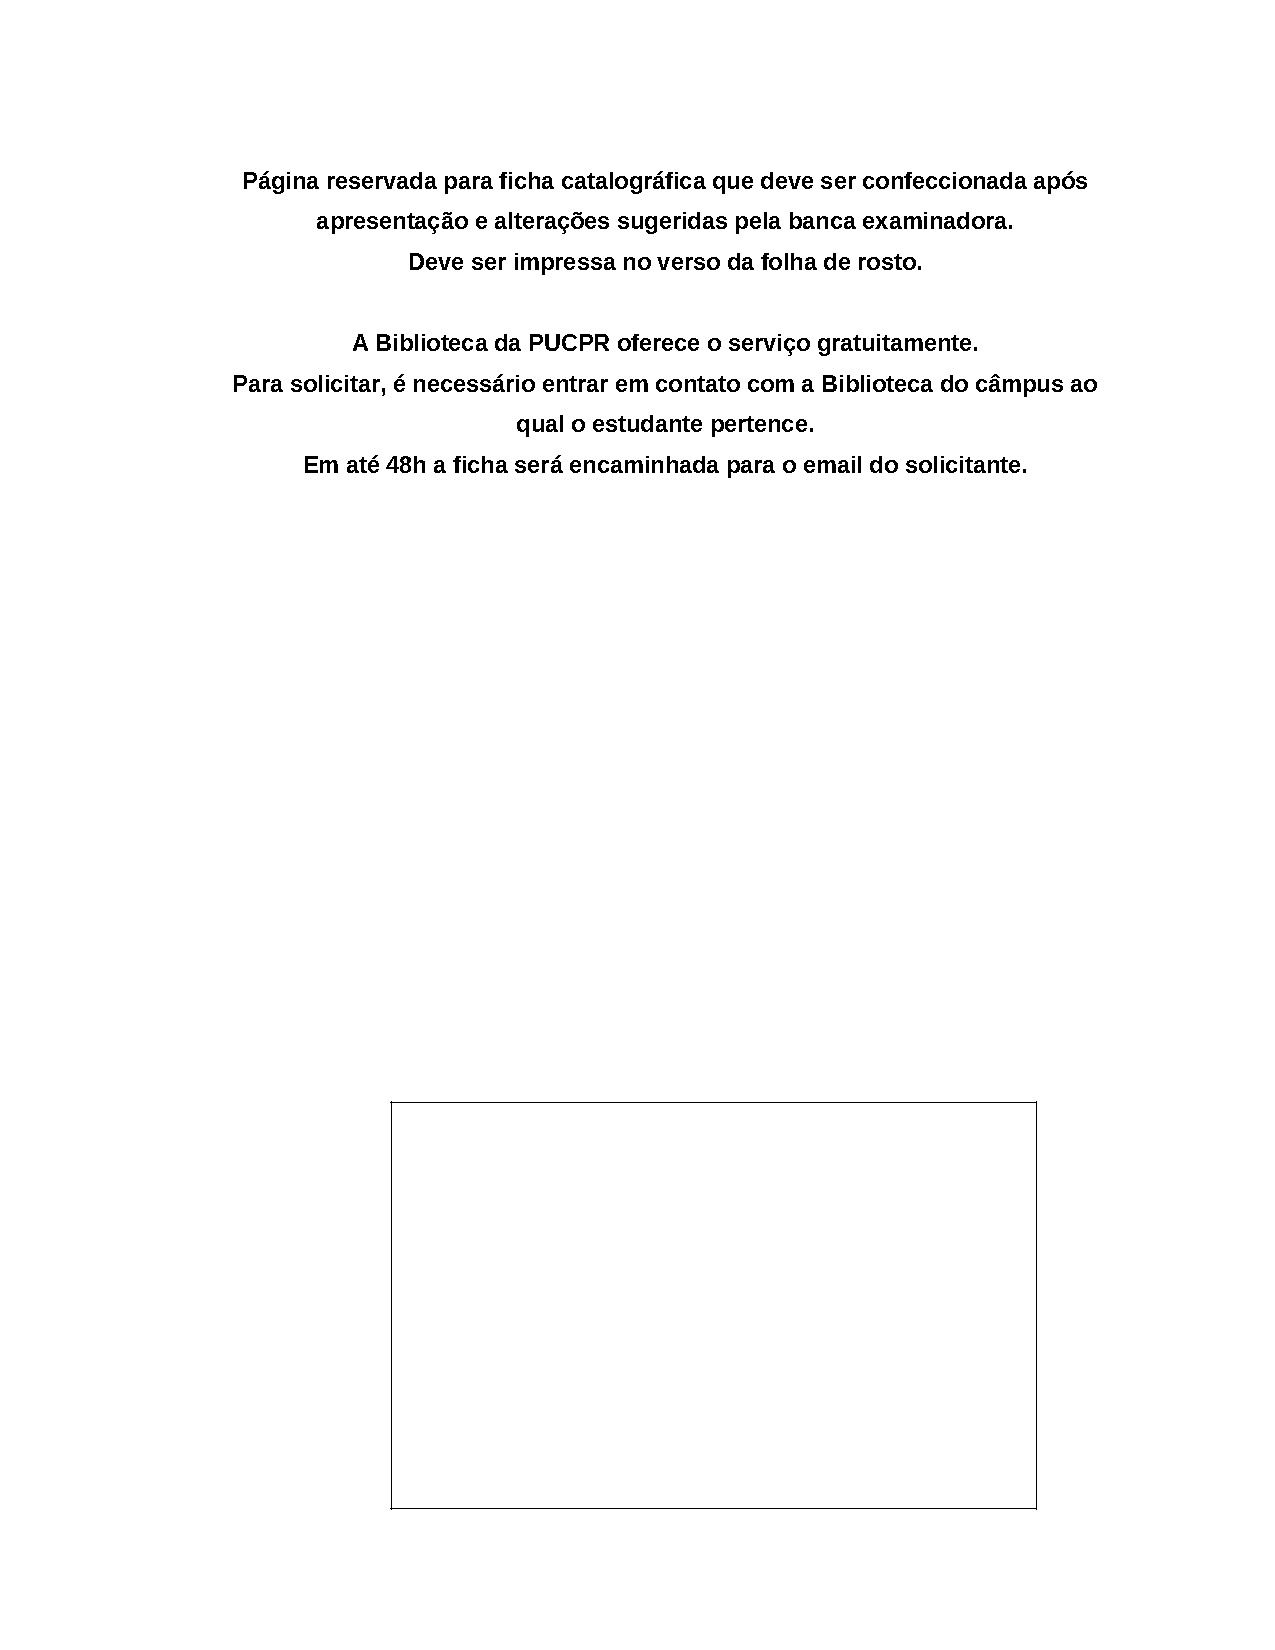
\includepdf{pdfs/ficha_catalografica.pdf}
\end{fichacatalografica}

%----------------------Folha de Aprovação----------------------%

% Após aprovação do trabalho, solicite do orientador a Folha de Aprovação assinada pela Banca Examinadora.
% Salve-a em formato PDF com o nome: folha_aprovacao.pdf
% Substitua o arquivo temporário de mesmo nome presente neste modelo.

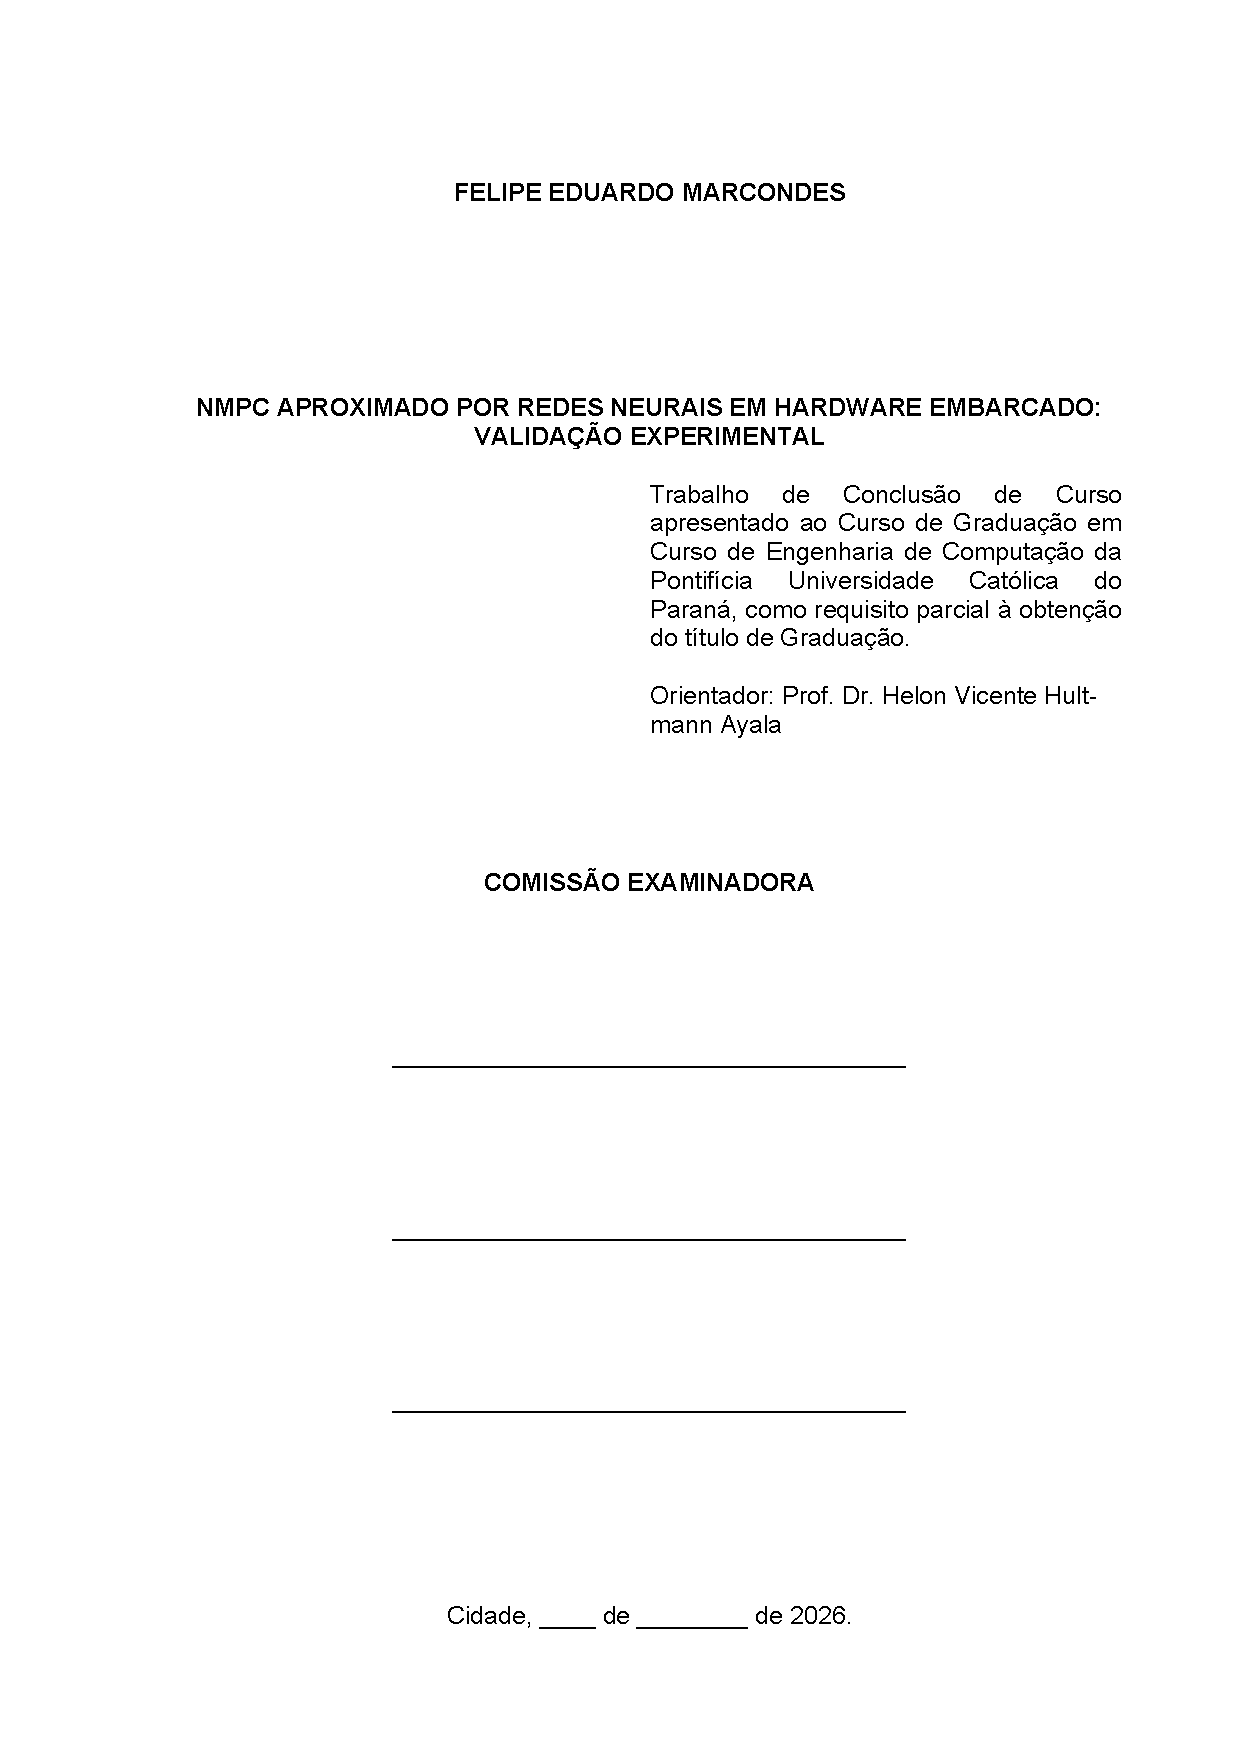
\includepdf{pdfs/folha-aprovacao.pdf}


%----------------------Dedicatória----------------------%
%\begin{dedicatoria}
%\vspace*{\fill}
%\begin{flushright}
%\begin{minipage}{8.5cm}
%\raggedleft
%\textit{
%A dedicatória deve ficar ao final da página e alinhada à direita.
%}
%\end{minipage}
%\end{flushright}
%\end{dedicatoria}



%----------------------Agradecimentos----------------------%
%\begin{agradecimentos}


%Agradeço à Pontifícia Universidade Católica do Paraná...

%Agradeço também ao órgão de fomento XYZ...  

%Sou grato(a) ao(à) meu(minha) orientador(a)... 

%Por fim, mas não menos importante, agradeço aos familiares e amigos...

%\end{agradecimentos}




%----------------------Epígrafe----------------------%
%\begin{epigrafe}
%    \vspace*{\fill}
%    \begin{flushright}
%        \begin{minipage}{8.5cm}
%            \raggedleft
%            \textit{}
%        \end{minipage}
%    \end{flushright}
%\end{epigrafe}


%----------------------Resumos----------------------%
%-%---------------Resumo em Português----------------%
\begin{resumo}
\SingleSpacing

    \noindent Este trabalho propõe o desenvolvimento e a validação experimental de um controlador neural embarcado para o rastreamento angular de um aeropêndulo instrumentado, visando contornar o elevado custo computacional do Controle Preditivo Não-Linear (NMPC) tradicional em microcontroladores. O sistema, operado por um motor BLDC e monitorado por uma IMU, é modelado fenomenologicamente e tem seus parâmetros aerodinâmicos e de atrito estimados experimentalmente pelo método de \textit{multiple shooting}. Um controlador PID estabiliza a planta na coleta de dados e serve como linha de base. A otimização iterativa do NMPC é substituída pela inferência direta de uma rede neural Perceptron Multicamadas (MLP), treinada em PyTorch com um conjunto de dados gerado pela resolução offline do problema de controle ótimo via CasADi. O modelo neural resultante é compilado em linguagem C nativa pela ferramenta X-CUBE-AI e executado em um microcontrolador STM32F446RE. O projeto avalia os compromissos entre a precisão do rastreamento de referências, a capacidade de rejeição a perturbações e as restrições de latência em tempo real ($T_s = 10$\,ms) e consumo de memória, comparando o desempenho da política neural embarcada com o controlador preditivo exato e a malha clássica.
    
    \vspace{\onelineskip}
    
    \noindent
    \textbf{Palavras-chave}: Aeropêndulo; Controle Preditivo Não-Linear; Redes Neurais Artificiais; Sistemas Embarcados; Identificação de Sistemas.
    
\end{resumo}

%----------------Resumo em Inglês----------------%
\begin{resumo}[\textbf{Abstract}]
\SingleSpacing
    \begin{otherlanguage*}{english}
    
        \noindent This work proposes the development and experimental validation of an embedded neural controller for the angular tracking of an instrumented aeropendulum, aiming to circumvent the high computational cost of traditional Nonlinear Model Predictive Control (NMPC) on microcontrollers. The system, driven by a BLDC motor and monitored by an IMU, is modeled phenomenologically and its aerodynamic and friction parameters are experimentally estimated using the multiple shooting method. A PID controller stabilizes the plant during data collection and serves as a baseline. The iterative optimization of the NMPC is replaced by the direct inference of a Multilayer Perceptron (MLP) neural network, trained in PyTorch with a dataset generated by the offline resolution of the optimal control problem via CasADi. The resulting neural model is compiled into native C code by the X-CUBE-AI tool and executed on an STM32F446RE microcontroller. The project evaluates the trade-offs between reference tracking accuracy, disturbance rejection capabilities, and the constraints of real-time latency ($T_s = 10$\,ms) and memory footprint, comparing the performance of the embedded neural policy with the exact predictive controller and the classical loop.
        
        \vspace{\onelineskip}
        
        \noindent 
        \textbf{Keywords}: Aeropendulum; Nonlinear Model Predictive Control; Artificial Neural Networks; Embedded Systems; System Identification.
        
    \end{otherlanguage*}
\end{resumo}




%----------------Lista de Ilustrações----------------%
\pdfbookmark[0]{\listfigurename}{lof}
\listoffigures*
\cleardoublepage


%----------------Lista de Quadros----------------%
\pdfbookmark[0]{\listofquadrosname}{loq}
\listofquadros*
\cleardoublepage




%----------------Lista de Tabelas----------------%
\pdfbookmark[0]{\listtablename}{lot}
\listoftables*
\cleardoublepage

%----------------Lista de Gráficos ----------------%
\pdfbookmark[0]{\listplotname}{lop}
\listofplots*
\cleardoublepage

%--------Lista de abreviaturas e siglas---------%
\begin{siglas}
    \item[ADC] Conversor Analógico-Digital (\textit{Analog-to-Digital Converter})
    \item[BLDC] Motor de Corrente Contínua sem Escovas (\textit{Brushless Direct Current})
    \item[CLF] Função de Lyapunov de Controle (\textit{Control Lyapunov Function})
    \item[DAG] Grafo Direcionado Acíclico (\textit{Directed Acyclic Graph} / Grafo de expressão simbólica)
    \item[Diffrax] Biblioteca para solução numérica diferenciável de equações diferenciais
    \item[DLPF] Filtro Passa-Baixas Digital (\textit{Digital Low-Pass Filter})
    \item[DMA] Acesso Direto à Memória (\textit{Direct Memory Access})
    \item[DNN] Rede Neural Profunda (\textit{Deep Neural Network})
    \item[dps] Graus por segundo (\textit{degrees per second})
    \item[EMPC] Controle Preditivo Baseado em Modelo Explícito (\textit{Explicit MPC})
    \item[ESC] Controlador Eletrônico de Velocidade (\textit{Electronic Speed Controller})
    \item[FFNN] Rede Neural \textit{Feedforward} (\textit{Feedforward Neural Network})
    \item[FPU] Unidade de Ponto Flutuante (\textit{Floating-Point Unit})
    \item[I$^2$C] \textit{Inter-Integrated Circuit}
    \item[IMU] Unidade de Medição Inercial (\textit{Inertial Measurement Unit})
    \item[JAX] Estrutura computacional para diferenciação automática e computação numérica de alta performance
    \item[MAE] Erro Absoluto Médio (\textit{Mean Absolute Error})
    \item[MCU] Microcontrolador (\textit{Microcontroller Unit})
    \item[MDF] \textit{Medium Density Fiberboard}
    \item[MEMS] Sistemas Microeletromecânicos (\textit{Micro-Electro-Mechanical Systems})
    \item[MLP] Perceptron Multicamadas (\textit{Multilayer Perceptron})
    \item[MPC] Controle Preditivo Baseado em Modelo (\textit{Model Predictive Control})
    \item[MSE] Erro Quadrático Médio (\textit{Mean Squared Error})
    \item[NLP] Programação Não-Linear (\textit{Nonlinear Programming})
    \item[NMPC] Controle Preditivo Não-Linear (\textit{Nonlinear Model Predictive Control})
    \item[OCP] Problema de Controle Ótimo (\textit{Optimal Control Problem})
    \item[ODE] Equação Diferencial Ordinária (\textit{Ordinary Differential Equation})
    \item[PID] Proporcional-Integral-Derivativo
    \item[PINN] Rede Neural Informada pela Física (\textit{Physics-Informed Neural Network})
    \item[PLA] Poliácido Láctico
    \item[PWA] Função Afim por Partes (\textit{Piecewise Affine})
    \item[PWM] Modulação por Largura de Pulso (\textit{Pulse Width Modulation})
    \item[QFN] \textit{Quad Flat No-leads}
    \item[ReLU] Unidade Linear Retificada (\textit{Rectified Linear Unit})
    \item[RMSE] Raiz do Erro Quadrático Médio (\textit{Root Mean Square Error})
    \item[SLSQP] Programação Sequencial de Mínimos Quadrados (\textit{Sequential Least Squares Programming})
    \item[SRAM] Memória de Acesso Aleatório Estática (\textit{Static Random Access Memory})
    \item[TCC] Trabalho de Conclusão de Curso
    \item[TFLM] TensorFlow Lite Micro
    \item[TIM] Temporizador (\textit{Timer})
    \item[UART] Transmissor-Receptor Assíncrono Universal (\textit{Universal Asynchronous Receiver-Transmitter})
    \item[USART] Transmissor-Receptor Síncrono e Assíncrono Universal (\textit{Universal Synchronous and Asynchronous Receiver-Transmitter})
    \item[VANT] Veículo Aéreo Não Tripulado
    \item[VTOL] Decolagem e Aterrissagem Vertical (\textit{Vertical Take-Off and Landing})
    \item[ZOH] Segurador de Ordem Zero (\textit{Zero-Order Hold})
\end{siglas}

%----------------Lista de Símbolos----------------%
\begin{simbolos}
    \item[$ \alpha $] Fator do filtro complementar
    \item[$ b $] Coeficiente de atrito viscoso
    \item[$ \mathcal{D} $] Conjunto de dados (\textit{dataset}) de treinamento
    \item[$ e $] Erro de rastreamento
    \item[$ f(\cdot) $] Função de transição de estados (dinâmica não-linear)
    \item[$ g $] Aceleração da gravidade
    \item[$ J $] Momento de inércia total do aeropêndulo
    \item[$ K_p, K_i, K_d $] Ganhos proporcional, integral e derivativo do controlador PID
    \item[$ K_\tau $] Constante de empuxo do motor
    \item[$ \kappa_N(\cdot) $] Lei de controle implícita do NMPC
    \item[$ L_1 $] Distância do conjunto motor-hélice ao pivô de rotação
    \item[$ L_2 $] Distância do contrapeso ao pivô de rotação
    \item[$ \ell(\cdot) $] Função de custo de estágio
    \item[$ M $] Número de intervalos no método \textit{multiple shooting}
    \item[$ m_1 $] Massa do conjunto motor-hélice
    \item[$ m_2 $] Massa do contrapeso
    \item[$ N $] Horizonte de predição
    \item[$ P $] Matriz de peso do custo terminal
    \item[$ Q $] Matriz de peso dos estados no custo de estágio
    \item[$ R $] Matriz de peso da ação de controle no custo de estágio
    \item[$ r $] Sinal de referência
    \item[$ s_i $] Variável de estado inicial local no método \textit{multiple shooting}
    \item[$ \theta $] Posição angular do braço do aeropêndulo
    \item[$ \dot{\theta} $] Velocidade angular
    \item[$ \ddot{\theta} $] Aceleração angular
    \item[$ \hat{\theta} $] Vetor de parâmetros a estimar
    \item[$ T_s $] Período de amostragem
    \item[$ \tau $] Torque gerado pelo empuxo do motor
    \item[$ U_k $] Sequência de controle a otimizar
    \item[$ u $] Sinal de controle (\textit{duty cycle} do PWM)
    \item[$ V_f(\cdot) $] Função de custo terminal
    \item[$ V_N^0(\cdot) $] Função de valor ótimo
    \item[$ x $] Vetor de estados do sistema
    \item[$ \mathcal{X} $] Conjunto admissível de estados / Conjunto de variáveis de decisão
    \item[$ \mathcal{X}_f $] Conjunto terminal
    \item[$ \mathcal{X}_N $] Domínio de factibilidade do Problema de Controle Ótimo
    \item[$ y $] Variável de processo observada
\end{simbolos}


%----------------SUMÁRIO----------------%
\pdfbookmark[0]{\contentsname}{toc}
\tableofcontents*
\cleardoublepage

%----------------------ELEMENTOS TEXTUAIS----------------------%
\textual
\pagestyle{simple}
%----------------Cap_01----------------%
\chapter{Introdução}

% ------------------------------------------------------------
% Contextualização
% ------------------------------------------------------------
O crescimento acelerado dos veículos aéreos não tripulados (VANTs) nas últimas décadas transformou setores como logística, monitoramento ambiental, agricultura de precisão e defesa. Plataformas de decolagem e aterrissagem vertical (VTOL), em particular os quadrotores, tornaram-se objetos de intensa investigação em razão de suas capacidades únicas de manobra, todavia impõem desafios igualmente expressivos de controle: dinâmica intrínsecamente não-linear, acoplamento entre eixos e forte sensibilidade a perturbações externas como rajadas de vento \cite{nguyen2020}. A operação segura e eficiente dessas plataformas exige algoritmos capazes de satisfazer simultaneamente requisitos de precisão de rastreamento, rejeição robusta a perturbações e execução em tempo real sob severas restrições computacionais dos microcontroladores embarcados.

Nesse contexto, o aeropêndulo consolida-se como uma bancada de experimentação, onde sistema reproduz a dinâmica essencial de um rotor VTOL em um único grau de liberdade, permitindo a comparação controlada de estratégias de controle em laboratório. Sua dinâmica não-linear, determinada pelo torque aerodinâmico do conjunto motor-hélice e pela não-linearidade gravitacional intrínseca ao pêndulo, exige técnicas de controle além dos métodos lineares clássicos. A bancada utilizada neste trabalho foi originalmente projetada e construída por \citeonline{lima2025}, cujo sistema mecânico e eletrônico é reaproveitado e estendido com novos algoritmos de controle.

% ------------------------------------------------------------
% Motivação / Justificativa
% ------------------------------------------------------------
O Controle Preditivo Não-Linear (NMPC) destaca-se entre as estratégias avançadas por combinar tratamento explícito de restrições, previsão do comportamento futuro da planta e desempenho reconhecidamente superior ao PID clássico em sistemas não-lineares \cite{mayne2000}. No entanto, a solução repetida de um Problema de Controle Ótimo a cada período de amostragem implica um custo computacional que pode ultrapassar os recursos disponíveis em microcontroladores de baixo custo operando em dinâmicas rápidas. Plataformas VTOL de pequeno porte tipicamente exigem períodos de amostragem da ordem de 10\,ms, intervalo que representa uma barreira prática para a implantação direta do NMPC em unidades de baixo poder computacional.

A abordagem de MPC aproximado por redes neurais surge como alternativa promissora, uma rede treinada offline para imitar a política do NMPC pode ser avaliada em tempo de inferência constante e reduzido, compatível com microcontroladores de classe Cortex-M \cite{karg2020}. A substituição da otimização repetida por uma única passagem \textit{feedforward} reduz o custo computacional em ordens de grandeza sem exigir reformulação do modelo ou dos objetivos de controle, tornando a estratégia particularmente atrativa para implantação embarcada em sistemas com restrições rígidas de memória e tempo \cite{david2021}.

% ------------------------------------------------------------
% Revisão da Literatura
% ------------------------------------------------------------
\section{Estado da Arte}

\subsection{Controle clássico}
Controladores clássicos como o PID (Proporcional-Integral-Derivativo) são a espinha dorsal de inúmeras aplicações industriais e robóticas. O desenvolvimento formal dessa lei de controle, também conhecida como controle de três termos, foi apresentado em 1922 pelo engenheiro Nicolas Minorsky \cite{bennett1996}.

Em plataformas ágeis, como VANTs, o controle PID muitas vezes não é suficiente de forma isolada, sendo relegado a uma malha interna de controle de atitude ou velocidade, o que cria a necessidade de controladores externos mais sofisticados capazes de garantir estabilidade sistêmica otimizada. Esse cenário motiva a adoção de algoritmos mais avançados, como o Controle Preditivo Baseado em Modelo (MPC), capaz de gerenciar diretamente sistemas de múltiplas entradas e múltiplas saídas com restrições operacionais rígidas \cite{nguyen2020}.

\subsection{Controle Preditivo Não-Linear}
O Controle Preditivo Não-Linear (NMPC) fundamenta-se na resolução de um problema de controle ótimo em tempo discreto e horizonte finito, em que um otimizador avalia um modelo preditivo para minimizar uma função de custo ao longo do horizonte de predição, lidando ativamente com restrições de estado e entrada. Uma de suas maiores vantagens em relação ao PID clássico é a característica de \textit{preview} (visão antecipada), pela qual o controlador avalia o comportamento futuro e reage a referências antes mesmo do erro se acumular \cite{mayne2000}. Embora o elevado custo computacional de resolver iterativamente online o problema de Programação Não-Linear (NLP) seja um desafio para o hardware embarcado, a adoção de métodos de otimização diretos reduz drasticamente a carga de processamento, viabilizando a aplicação do NMPC mesmo na dinâmica inerentemente rápida de robôs aéreos \cite{nguyen2020}.

\subsection{MPC Explícito e suas limitações}
Buscando contornar o custo computacional da otimização online, surgiu o conceito de MPC Explícito (EMPC). Nessa abordagem, a lei de controle é pré-computada offline por meio da resolução de um problema de programação multiparamétrica, resultando em uma função afim por partes (PWA) definida sobre partições politópicas do espaço de estados, a execução online resume-se, então, a identificar o polítopo atual e aplicar a equação correspondente \cite{bemporad2002}. A principal limitação de escalabilidade do EMPC reside no crescimento exponencial do número de regiões politópicas à medida que o horizonte de predição e o número de restrições aumentam, tornando sua aplicação em sistemas embarcados restrita a problemas de baixíssima dimensionalidade \cite{bemporad2002}. Esse gargalo motiva fortemente a adoção de abordagens de aproximação da lei de controle por inteligência artificial, como o uso de redes neurais \cite{alsmeier2024}.

\subsection{Aproximação de leis de controle por redes neurais}
A limitação de escalabilidade de memória do EMPC impulsiona a aproximação da sua lei de controle explícita por uma rede neural previamente treinada. \citeonline{karg2020} demonstraram matematicamente que Redes Neurais Profundas (DNNs) com funções de ativação ReLU conseguem representar de maneira exata as funções afins por partes das leis de controle do MPC. O principal desafio técnico desta abordagem recai sobre o erro de aproximação e a perda de garantias intrínsecas do MPC original. Para lidar com os \textit{trade-offs} entre tamanho do modelo e segurança, pesquisadores aplicam a Desigualdade de Hoeffding para conferir limites estatísticos e garantir a satisfação de restrições com alta probabilidade \cite{hertneck2018}; alternativamente, derivam-se limites no pior caso via constantes de Lipschitz para certificar que os desvios da rede em relação à lei nominal estão contidos no limite de robustez
\cite{alsmeier2024}.

\subsection{Identificação de sistemas para alimentar o NMPC}
Para a concepção offline de um projeto de NMPC, a precisão do modelo preditivo subjacente é vital para as predições de estados. Muitos sistemas, como motores BLDC em um aeropêndulo, exibem atritos e aerodinâmicas difíceis de modelar analiticamente. Nesses casos, a identificação baseada em dados de entrada e saída torna-se altamente efetiva. A partir de ensaios experimentais, é possível treinar modelos de predição que capturam os efeitos dinâmicos dominantes, incluindo não-linearidades aerodinâmicas negligenciadas pelos modelos físicos clássicos, e integrá-los diretamente ao esquema MPC \cite{jiang2022}.

\subsection{Redes neurais MLP arquitetura e treinamento supervisionado} A fim de aproximar a política de controle, as Redes Neurais \textit{Feedforward} (FFNN), ou Perceptrons Multicamadas (MLP), mostram-se candidatas ideais devido à sua capacidade de mapeamento estático livre de \textit{delays} recorrentes. A arquitetura típica consiste em camadas ocultas com funções de ativação ReLU e uma camada de saída linear. A geração do \textit{dataset} se da pela exploração em malha fechada do controlador MPC exato sobre estados iniciais diversos, registrando-se os pares de ``estado atual'' $\rightarrow$ ``ação de controle ótima''; o treinamento subsequente ocorre com aprendizado supervisionado focado em minimizar o Erro Quadrático Médio (MSE), por meio de algoritmos baseados em descida de gradiente estocástico, como o otimizador Adam \cite{karg2020}.

\subsection{Inferência de redes neurais em hardware embarcado (TinyML)} Executar algoritmos preditivos em microcontroladores (MCUs) requer superar restrições críticas de memória e frequência de relógio típicas do domínio TinyML. Sem o suporte de sistemas operacionais tradicionais, bibliotecas padronizadas frequentemente não operam adequadamente nesses hardwares. \textit{Frameworks} focados como o TensorFlow Lite Micro (TFLM) fornecem a base necessária, operando em poucas dezenas de kilobytes para viabilizar a inferência profunda em dispositivos restritos. Ferramentas comerciais dedicadas, como a extensão \texttt{STM32Cube.AI} da STMicroelectronics, convertem as matrizes geradas no treinamento (TensorFlow/Keras) em código C otimizado e quantizado para a família STM32 \cite{david2021}.

\subsection{Trabalhos relacionados e lacuna identificada}
Trabalhos recentes evidenciam a convergência das redes neurais no controle MPC. \citeonline{jiang2022} utilizaram uma rede FFNN estritamente como modelo de dinâmica translacional preditiva em tempo real dentro de um MPC. Similarmente, \citeonline{sanyal2024} formularam a RAMP-Net, que emprega Redes Neurais Informadas pela Física (PINNs) para compensar distúrbios em um sistema NMPC de drones. \citeonline{li2024} propuseram estratégias diretas na variedade topológica $SO(3)$ com um Learning-MPC, exigindo, contudo, hardware veicular de alta capacidade para operação em tempo real.
% ============================================================
\section{Objetivos}

\subsection{Objetivo Geral}

Desenvolver e validar experimentalmente um controlador neural embarcado que aproxima a política de controle ótima de um NMPC para rastreamento angular de um aeropêndulo instrumentado, demonstrando viabilidade de implantação em tempo real no microcontrolador com desempenho comparável ao controlador preditivo exato.

\subsection{Objetivos Específicos}

Os objetivos específicos do trabalho são:

\begin{enumerate}
    \item sintetizar um controlador PID como referência de desempenho e para estabilização da planta durante os ensaios de identificação;
    \item identificar os parâmetros do modelo dinâmico grey-box do aeropêndulo por meio de ensaios experimentais, obtendo um modelo validado para síntese de controladores;
    \item formular e resolver offline o Problema de Controle Ótimo do NMPC, gerando a política ótima e o \textit{dataset} de treinamento da rede neural;
    \item treinar uma rede MLP para aproximar a política do NMPC e implantar o modelo resultante na bancada;
    \item comparar experimentalmente os três controladores, PID, NMPC e MLP embarcada em termos de desempenho de rastreamento, rejeição a perturbações e custo computacional em hardware embarcado.
\end{enumerate}
%----------------Cap_02----------------%
\chapter{Fundamentação Teórica e Estado da Arte}
\label{cap:fundamentacao}

Este capítulo estabelece a base teórica e conceitual que fundamenta o desenvolvimento deste trabalho, cobrindo os princípios do controle clássico, a formulação do controle preditivo não-linear, os métodos de identificação de sistemas dinâmicos e as técnicas de inteligência computacional embarcada (\textit{TinyML}) empregadas para a aproximação de políticas ótimas. Ao final, revisam-se os trabalhos correlatos recentes na literatura e evidencia-se a lacuna científica e tecnológica abordada pela pesquisa.

% ============================================================
\section{Controle Clássico}
\label{sec:fund_classico}
% ============================================================

Controladores clássicos como o PID (Proporcional-Integral-Derivativo) constituem a espinha dorsal de inúmeras aplicações industriais e robóticas. O desenvolvimento formal dessa lei de controle, também conhecida como controle de três termos, foi apresentado em 1922 pelo engenheiro Nicolas Minorsky \cite{bennett1996}.

Em plataformas ágeis, como os Veículos Aéreos Não Tripulados (VANTs), o controle PID muitas vezes não é suficiente de forma isolada, sendo frequentemente relegado a uma malha interna rápida de estabilização de atitude ou de velocidade angular. Essa limitação decorre de sua incapacidade intrínseca de considerar restrições operacionais explícitas nos atuadores (como saturações de empuxo) e de antecipar dinâmicas futuras não-lineares, criando a necessidade de estratégias preditivas mais avançadas capazes de gerenciar sistemas com dinâmicas acopladas e restrições físicas rígidas \cite{nguyen2020}.

% ============================================================
\section{Controle Preditivo Não-Linear (NMPC)}
\label{sec:fund_nmpc}
% ============================================================

O Controle Preditivo Não-Linear (NMPC) fundamenta-se na resolução repetida, a cada período de amostragem, de um problema de controle ótimo em tempo discreto e horizonte finito. Um otimizador numérico propaga um modelo preditivo não-linear da planta para calcular uma sequência de controle que minimiza uma função de custo quadrática acumulada, respeitando ativamente restrições de estado e de entrada \cite{mayne2000, rawlings2017}.

Uma das maiores vantagens do NMPC em relação às malhas lineares clássicas reside na característica de \textit{preview} (visão antecipada da referência futura): ao conhecer a trajetória desejada ao longo do horizonte $N$, o controlador inicia a aceleração ou frenagem de maneira preventiva antes que o erro de rastreamento se acumule. Todavia, a resolução iterativa online de um Problema de Programação Não-Linear (NLP) impõe elevado custo computacional, tornando sua aplicação direta em microcontroladores de baixo custo um desafio expressivo em sistemas com dinâmicas rápidas \cite{nguyen2020}.

% ============================================================
\section{MPC Explícito e suas Limitações}
\label{sec:fund_empc}
% ============================================================

Buscando contornar a sobrecarga computacional da otimização numérica online, propôs-se o conceito de MPC Explícito (EMPC). Nessa formulação, o problema de controle ótimo sob restrições lineares é resolvido parametricamente offline por meio de programação multiparamétrica. A lei de controle resultante é expressa como uma função afim por partes (\textit{Piecewise Affine} - PWA) definida sobre partições politópicas do espaço de estados, de modo que a avaliação online restringe-se à busca pontual do polítopo ativo e à avaliação de uma equação linear simples \cite{bemporad2002}.

Apesar de eliminar os resolvedores iterativos no hardware embarcado, o EMPC sofre de um severo problema de escalabilidade dimensional: o número de partições politópicas cresce exponencialmente com o horizonte de predição e com a quantidade de restrições ativas. Essa explosão combinatória inviabiliza o armazenamento da tabela de polítopos na memória estática de microcontroladores para sistemas de ordem média ou com horizontes estendidos \cite{bemporad2002}. Tal limitação estimula a exploração de técnicas de aprendizado de máquina como aproximadores de função com consumo de memória determinístico \cite{alsmeier2024}.

% ============================================================
\section{Aproximação de Leis de Controle por Redes Neurais}
\label{sec:fund_ann_mpc}
% ============================================================

A necessidade de contornar as restrições de memória do EMPC impulsiona o emprego de Redes Neurais Artificiais para aprender a política ótima de controle. Formalmente, \citeonline{karg2020} demonstraram que Redes Neurais Profundas (DNNs) com funções de ativação do tipo ReLU (\textit{Rectified Linear Unit}) são estruturalmente capazes de representar de forma exata qualquer função afim por partes gerada por controladores preditivos lineares e aproximar funções contínuas arbitrárias decorrentes de NMPCs com alta fidelidade.

O desafio central dessa abordagem consiste no controle do erro de aproximação e na manutenção de salvaguardas de estabilidade. Para mitigar esses riscos, investigam-se abordagens estatísticas baseadas na Desigualdade de Hoeffding para certificar a satisfação de restrições com alta probabilidade \cite{hertneck2018}, além de métodos determinísticos baseados em constantes de Lipschitz para assegurar que as discrepâncias entre a inferência da rede e o comando ótimo nominal permaneçam limitadas dentro da margem de robustez do sistema \cite{alsmeier2024}.

% ============================================================
\section{Identificação de Sistemas para Alimentação do NMPC}
\label{sec:fund_sysid}
% ============================================================

A viabilidade prática e o desempenho de qualquer controlador preditivo dependem intrinsecamente da qualidade preditiva do modelo dinâmico utilizado. Em plantas mecatrônicas de aeropêndulo operadas por motores BLDC e hélices, fenômenos como atrito seco nos mancais, histerese aerodinâmica e efeitos de recirculação de ar são de difícil quantificação puramente fenomenológica.

Nesse contexto, as técnicas de Identificação de Sistemas orientadas a dados desempenham papel fundamental. A partir de ensaios dinâmicos em que o sistema é excitado por sinais com riqueza espectral persistente, identificam-se modelos não-lineares — como modelos autorregressivos com entradas exógenas (NARX) ou modelos de caixa cinza (\textit{grey-box}) ajustados via \textit{multiple shooting} —, permitindo alimentar o otimizador preditivo com representações fiéis do envelope operacional real \cite{jiang2022, billings2013}.

% ============================================================
\section{Redes Neurais Multicamadas (MLP)}
\label{sec:fund_mlp}
% ============================================================

Dentre as topologias neurais, as redes \textit{Feedforward} do tipo Perceptron Multicamadas (MLP) são especialmente adequadas para aproximar leis de controle preditivo em razão de seu tempo de execução estritamente determinístico e ausência de laços recorrentes internos. A rede é estruturada em uma camada de entrada que recebe o vetor de estados medidos, históricos passados e a trajetória de referências futuras (\textit{preview}), camadas ocultas densas com ativações ReLU e uma camada de saída linear que fornece o comando escalar de controle ótimo $u^*(k)$.

O treinamento é conduzido sob o paradigma supervisionado com a função de perda do Erro Quadrático Médio (MSE), utilizando algoritmos de otimização estocástica baseados em gradiente, como o Adam. O banco de dados de treinamento é gerado pela resolução offline do problema de controle ótimo em malha fechada cobrindo sistematicamente o espaço de estados de interesse \cite{karg2020, paszke2019}.

% ============================================================
\section{Inferência de Redes Neurais em Hardware Embarcado (TinyML)}
\label{sec:fund_tinyml}
% ============================================================

A implantação de modelos neurais em sistemas mecatrônicos de baixo custo e tempo real restrito insere-se no domínio do \textit{TinyML} (\textit{Tiny Machine Learning}). Em microcontroladores de classe ARM Cortex-M, os recursos de computação são severamente limitados: memórias SRAM da ordem de centenas de kilobytes, memória Flash de alguns megabytes e operação desprovida de sistema operacional de propósito geral.

Para atender a essas restrições, utilizam-se cadeias de ferramentas especializadas. Bibliotecas como o \textit{TensorFlow Lite for Microcontrollers} (TFLM) e extensões proprietárias como o \texttt{X-CUBE-AI} da STMicroelectronics analisam o grafo computacional da rede e o traduzem em código C nativo otimizado, explorando instruções vetoriais da biblioteca CMSIS-NN e unidades de ponto flutuante (FPU). Esse pipeline viabiliza inferências em frações de milissegundo, preservando a determinabilidade temporal requerida para malhas de controle de alta taxa de amostragem \cite{david2021}.

% ============================================================
\section{Trabalhos Correlatos e Lacuna Identificada}
\label{sec:fund_correlatos}
% ============================================================

A convergência entre aprendizado de máquina e controle preditivo tem sido explorada ativamente na literatura recente. \citeonline{jiang2022} aplicaram uma rede neural feedforward operando como modelo dinâmico preditivo acoplado a um otimizador online em um veículo aéreo, enfrentando ainda demandas computacionais consideráveis. Na linha de compensação de perturbações, \citeonline{sanyal2024} propuseram a arquitetura RAMP-Net, que combina Redes Neurais Informadas pela Física (PINNs) para absorver distúrbios de vento em NMPC de drones. Em trabalhos teóricos, \citeonline{li2024} investigaram o Learning-MPC diretamente no grupo de Lie $SO(3)$, exigindo computadores de bordo com GPUs dedicadas para processamento em tempo real.

Nota-se, contudo, que grande parte dos trabalhos foca na aceleração em computadores de bordo pesados ou limita-se à validação puramente simulada. Identifica-se uma expressiva lacuna tecnológica no que concerne ao **pipeline completo de ponta a ponta**: desde a identificação não-linear de uma bancada física real, passando pela síntese offline do NMPC e aproximação neural, até a implantação experimental determinística em microcontrolador de baixo custo (Cortex-M4 a 180\,MHz a 100\,Hz) com diagnóstico e superação do *Sim-to-Real gap*. É a essa lacuna que este trabalho se dedica.

%----------------Cap_03----------------%
\chapter{Metodologia e Desenvolvimento do Sistema}
\label{cap:metodologia}
 
Este capítulo apresenta o detalhamento completo da fase experimental do projeto, cobrindo a descrição do sistema físico, a modelagem e identificação do modelo dinâmico e a implementação do controlador no hardware embarcado. A arquitetura da solução está sintetizada no diagrama de blocos da Figura~\ref{fig:diagrama-blocos-projeto}, que organiza o desenvolvimento em duas fases.
 
\begin{figure}[H]
    \centering
    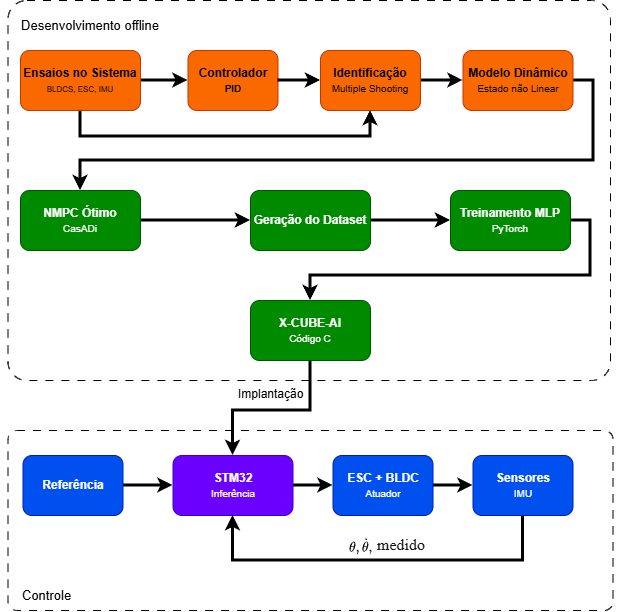
\includegraphics[width=1\textwidth]{img/blocos-projeto.png}
    \caption{Diagrama de Blocos do Projeto}
    \label{fig:diagrama-blocos-projeto}
\end{figure}

 A fase offline corresponde: (i)~a síntese e implantação do controlador PID em malha fechada, utilizado tanto para estabilizar a planta durante a coleta de dados quanto como referência de desempenho na comparação final (Seção~\ref{sec:pid}); (ii)~a aquisição dos dados de identificação em malha fechada com o PID ativo e a estimação dos parâmetros do modelo dinâmico via \textit{multiple shooting} (Seção~\ref{sec:identificacao}); (iii)~a formulação e resolução do NMPC via CasADi, a geração do \textit{dataset} e o treinamento da rede neural MLP (Seção~\ref{sec:sintese}). A fase de operação em tempo real, na parte inferior, corresponde à implantação do controlador embarcado no STM32 e sua atuação sobre a planta física (Seção~\ref{sec:embarcado}). A Seção~\ref{sec:descricao_fisica} descreve a bancada e os componentes de hardware que suportam ambas as fases.
 
% ------------------------------------------------------------
\section{Descrição do Sistema Físico}
\label{sec:descricao_fisica}
A infraestrutura física e mecânica da bancada do aeropêndulo utilizada neste trabalho foi originalmente projetada e construída por \citeonline{lima2025}. O sistema mecânico pré-existente e reaproveitado compreende a base de madeira, as torres de suporte, o eixo de alumínio instrumentado e a haste pendular contendo o motor \textit{brushless} (BLDC) acoplado.

O aeropêndulo atua como um sistema de um grau de liberdade, composto por esse braço rígido livre para rotacionar em torno do eixo horizontal fixo. A posição angular $\theta$ é medida em relação à horizontal, sendo $0^\circ$ definido quando o sistema está em repouso com o motor na posição inferior.

% ------------------------------------------------------------
\subsection{Estrutura Mecânica}

A estrutura física do aeropêndulo é montada sobre uma base de madeira compensada. Dois suportes triangulares confeccionados em MDF sustentam o eixo de rotação do sistema. As faces foram unidas por colagem nas arestas, e peças impressas em 3D foram fixadas nos cantos de cada torre e parafusadas à base.

Para fixar o eixo de alumínio às torres, é utilizado um cuboide retangular contendo um rolamento de esferas, permitindo que o eixo gire livremente. No centro do eixo foi usinado e rosqueado um furo para encaixe da haste do pêndulo.

A haste rosqueada também permite a fixação e remoção facilitada de contrapesos, que foram usinados e rosqueados para se encaixar diretamente na haste. Um suporte impresso em 3D acopla o motor BLDC à extremidade da haste. A propulsão é gerada por uma hélice bipá de passo fixo. Um alojamento impresso em 3D para a Unidade de Medição Inercial (IMU) foi desenvolvido e fixado ao eixo de rotação, responsável por capturar o ângulo do sistema. A Figura~\ref{fig:montagem-bancada} ilustra o formato atual da bancada. Os principais parâmetros construtivos do sistema são resumidos na Tabela~\ref{tab:componentes_mecanicos}.

\begin{figure}[h]
    \centering
    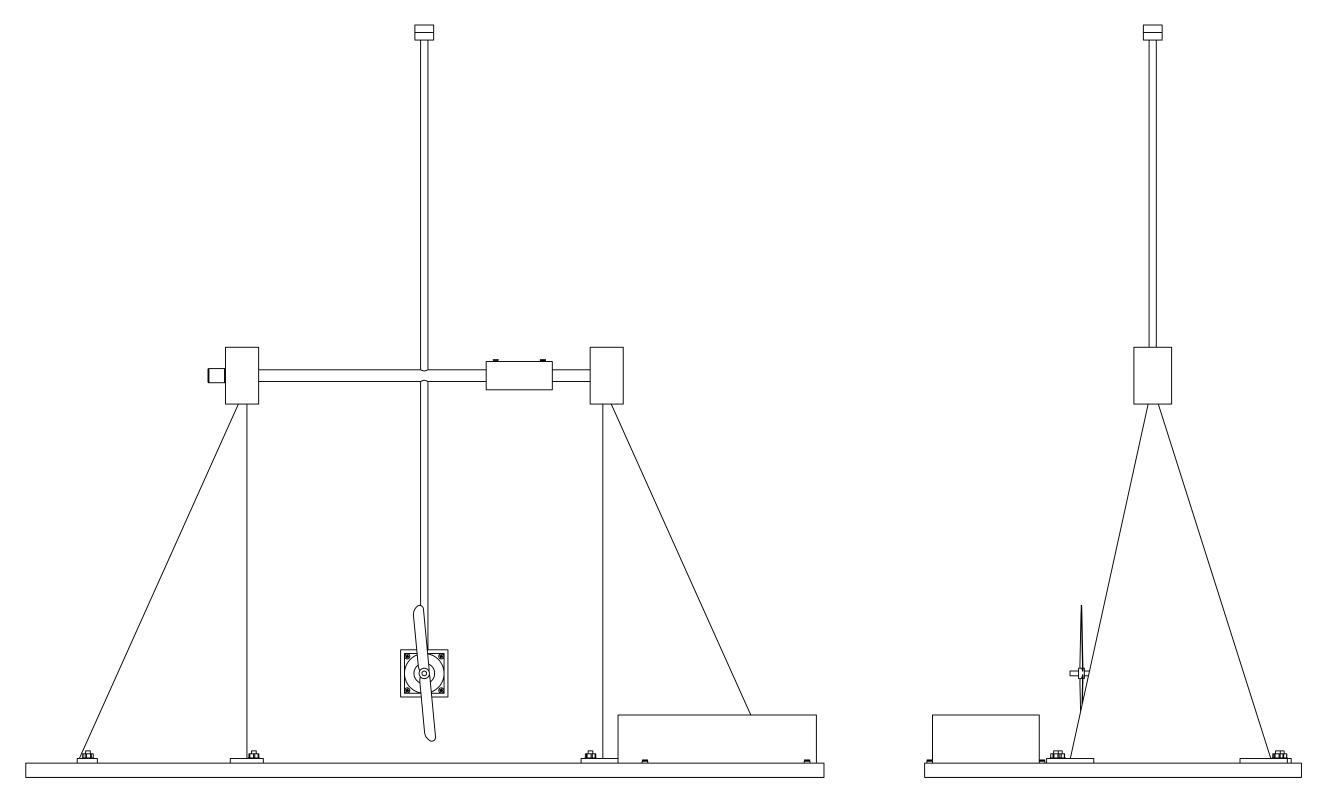
\includegraphics[width=1\textwidth]{img/montagem-bancada.png}
    \caption{Desenho da Bancada}
    \label{fig:montagem-bancada}
\end{figure}

\begin{table}[h!]
    \centering
    \caption{Componentes mecânicos do aeropêndulo}
    \label{tab:componentes_mecanicos}
    \begin{tabular}{ll}
        \hline
        \textbf{Componente}       & \textbf{Material / Modelo}              \\
        \hline
        Base                      & Madeira compensada                      \\
        Torres de suporte         & MDF com reforços em PLA (impressão 3D)  \\
        Eixo de rotação           & Alumínio                                \\
        Mancal                    & Rolamento de esferas                    \\
        Haste do pêndulo          & Haste rosqueada                         \\
        Contrapesos               & Peças rosqueadas (ajustáveis)           \\
        Suporte do motor          & PLA (impressão 3D)                      \\
        Alojamento da IMU         & PLA (impressão 3D)                      \\
        Motor                     & EMAX RS2306                             \\
        Hélice                    & Bipá, passo fixo                        \\
        \hline
    \end{tabular}
\end{table}

% ------------------------------------------------------------
\subsection{Sensores}

% ------------------------------------------------------------
\subsubsection{Unidade de Medição Inercial (IMU)}

A unidade de medição inercial utilizada é o ICM-20948, fabricado pela InvenSense (TDK), um dispositivo MEMS de 9 eixos que integra giroscópio triaxial, acelerômetro triaxial e magnetômetro triaxial em um único encapsulamento QFN de 3$\times$3$\times$1\,mm \cite{invensense2021icm20948}.

A comunicação com o microcontrolador é realizada via I$^2$C no modo \textit{fast} (400\,kHz), utilizando os pinos SCL e SDA do STM32. O endereço I$^2$C do dispositivo é definido pelo nível lógico do pino AD0, com AD0 em nível baixo, o endereço é \texttt{0x68}. Os dados do giroscópio e do acelerômetro são utilizados em conjunto na estimação do ângulo gerado pelo braço do aeropêndulo.

O giroscópio apresenta fundo de escala programável de $\pm250$, $\pm500$, $\pm1000$ ou $\pm2000$\,dps, com ADC de 16 bits e sensibilidade de 131\,LSB/dps na configuração de menor fundo de escala. A densidade espectral de ruído típica é de 0,015\,dps/$\sqrt{\text{Hz}}$, e o filtro passa-baixas digital (DLPF) é configurável entre 5,7 e 197\,Hz \cite{invensense2021icm20948}. A Tabela~\ref{tab:icm_gyro} resume os parâmetros do giroscópio que são relevantes para a aplicação.

\begin{table}[h]
    \centering
    \caption{Parâmetros do giroscópio do ICM-20948 utilizados no projeto.}
    \label{tab:icm_gyro}
    \begin{tabular}{lcc}
        \hline
        \textbf{Parâmetro} & \textbf{Valor} & \textbf{Unidade} \\
        \hline
        Fundo de escala selecionado & $\pm500$ & dps \\
        Sensibilidade                & 65,5   & LSB/dps \\
        Resolução do ADC             & 16     & bits \\
        Frequência de amostragem     & 100    & Hz \\
        Largura de banda do DLPF     & 51,2   & Hz \\
        Interface de comunicação     & I$^2$C & {-} \\
        Tensão de alimentação (VDD)  & 3,3    & V \\
        \hline
    \end{tabular}
\end{table}

A frequência de amostragem de 100\,Hz satisfaz o requisito de $T_s \leq 10$\,ms imposto pela dinâmica do aeropêndulo, e a largura de banda do filtro de 51,2\,Hz é suficiente para capturar os modos dinâmicos relevantes sem amplificar ruído de alta frequência.

A leitura dos registradores de saída do giroscópio é executada via interrupção de timer no STM32, garantindo periodicidade determinística.

% ------------------------------------------------------------
\subsection{Microcontrolador STM32 Nucleo-F446RE}

O núcleo de processamento do aeropêndulo é composto pelo microcontrolador STM32F446, baseado na arquitetura Arm Cortex-M4 de 32 bits, operando a uma frequência de clock máxima de 180\,MHz. Este processador incorpora uma Unidade de Ponto Flutuante (FPU) em hardware que suporta todas as instruções de precisão única do padrão IEEE 754, o que elimina a sobrecarga computacional de emulação por software e otimiza a execução em tempo real do algoritmo de controle do aeropêndulo e da filtragem dos sensores. A arquitetura de memória do dispositivo conta com 512\,KB de memória Flash para armazenamento do firmware e 128\,KB de memória SRAM para alocação dinâmica de variáveis e buffers de execução \cite{stm32}.

Os periféricos internos atendem aos requisitos dinâmicos e de interface do sistema, dividindo-se nas seguintes funções:

\begin{itemize}
    \item \textbf{Inter-Integrated Circuit (I$^2$C):} Barramento serial síncrono configurado no modo \textit{Fast Mode} (400\,kHz) para comunicação direta com a IMU ICM-20948, realizando a leitura periódica dos registradores do acelerômetro e giroscópio.
    \item \textbf{Temporizador (TIM):} Configurado em modo de geração de PWM (\textit{Pulse Width Modulation}) com resolução adequada para o acionamento do ESC (\textit{Electronic Speed Controller}), regulando de forma determinística a potência elétrica entregue ao motor \textit{brushless}.
    \item \textbf{Universal Asynchronous Receiver-Transmitter (UART):} Interface serial assíncrona estabelecida com taxa de transmissão elevada (ex.: 500.000\,baud) para o envio de telemetria em tempo real (ângulo estimado, erro, ação de controle) para o computador de ensaios e recepção de comandos de depuração.
\end{itemize}

A Tabela~\ref{tab:perifericos_stm32} especifica a atribuição física de pinos e periféricos utilizada na implementação do protótipo.

\begin{table}[h]
    \centering
    \caption{Mapeamento de periféricos e pinos do STM32F446 para o aeropêndulo.}
    \label{tab:perifericos_stm32}
    \begin{tabularx}{\textwidth}{llXX}
        \hline
        \textbf{Periférico} & \textbf{Pino} & \textbf{Função Configurada} & \textbf{Destino / Interface} \\
        \hline
        \\
        I2C1\_SCL  & PB8  & Clock do barramento I$^2$C (400\,kHz) & Pino SCL da IMU ICM-20948 \\
        I2C1\_SDA  & PB9  & Dados do barramento I$^2$C (400\,kHz) & Pino SDA da IMU ICM-20948 \\
        TIM1\_CH1  & PA8  & Saída PWM (Sinal de Controle) & Entrada de Sinal do ESC \\
        USART2\_TX & PA2  & Transmissão Serial Assíncrona & Receptor USB-UART \\
        USART2\_RX & PA3  & Recepção Serial Assíncrona    & Receptor USB-UART \\
        \hline
    \end{tabularx}
\end{table}

A Figura~\ref{fig:esquematico} apresenta o esquemático elétrico simplificado da bancada, ilustrando a interligação entre o STM32 Nucleo-F446RE, a IMU ICM-20948 e o ESC. A fonte de alimentação do motor (VBAT) é independente da 
alimentação lógica do microcontrolador.

\begin{figure}[h]
    \centering
    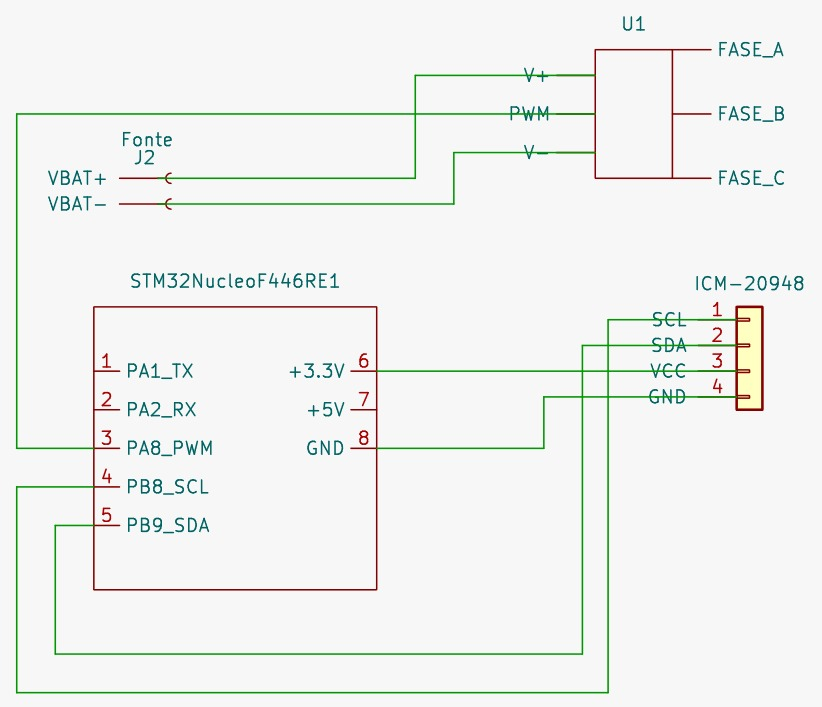
\includegraphics[width=1\textwidth]{img/diagrama-eletrico.png}
    \caption{Esquemático elétrico simplificado da bancada}
    \label{fig:esquematico}
\end{figure}

% ============================================================
\section{Identificação do Modelo Dinâmico}
\label{sec:identificacao}

A síntese do Controle Preditivo Não-Linear (NMPC) exige um modelo matemático rigoroso, mas a modelagem puramente analítica do aeropêndulo impõe dificuldades práticas, visto que parâmetros físicos são de difícil mensuração isolada e o arranjo motor-hélice introduz não-linearidades que costumam ser ignoradas. Contudo, as abordagens clássicas de identificação baseadas em modelos lineares possuem restrições estruturais que as tornam insuficientes para representar os efeitos aerodinâmicos em todo o envelope operacional da planta \cite{jiang2022}. 

Diante dessas limitações, adota-se uma abordagem híbrida: a estrutura do modelo é derivada analiticamente a partir dos princípios físicos do sistema, enquanto os parâmetros de difícil mensuração são estimados por identificação experimental. Pela Segunda Lei de Newton aplicada à dinâmica rotacional, considerando  explicitamente a massa do conjunto motor-hélice $m_1$ posicionada à distância  $L_1$ do pivô e a massa do contrapeso $m_2$ posicionada à distância $L_2$ no  lado oposto, a equação de movimento do aeropêndulo é:

\begin{equation}
    J\ddot{\theta} + b\dot{\theta} + (m_1 L_1 - m_2 L_2)\,g\sin(\theta) = \tau(u),
    \label{eq:dinamica}
\end{equation}
\noindent onde $\theta$ é o ângulo de inclinação em relação à vertical,  $\dot{\theta}$ a velocidade angular, $J$ o momento de inércia total, $b$ o  coeficiente de atrito viscoso, $g$ a aceleração da gravidade e $\tau(u)$ o  torque gerado pelo empuxo do motor em função do sinal de controle $u$. O termo  $(m_1 L_1 - m_2 L_2)\,g\sin(\theta)$ caracteriza a não-linearidade gravitacional  intrínseca ao sistema, cujo valor efetivo depende do balanço entre o torque  restaurador do motor e o torque compensatório do contrapeso, tornando inadequada  qualquer representação linear para operação em ampla faixa angular \cite{khalil2002}.

Para o formalismo do NMPC, é necessário representar o sistema na forma de  espaço de estados não-linear $\dot{x} = f(x, u)$. Definindo o vetor de estados  $x = [\theta,\;\dot{\theta}]^\top$ e isolando $\ddot{\theta}$ na  Equação~\ref{eq:dinamica}, obtém-se:

\begin{equation}
    \dot{x} = f(x,\, u) =
    \begin{bmatrix}
        \dot{\theta} \\[4pt]
        \dfrac{\tau(u) - b\dot{\theta} - (m_1 L_1 - m_2 L_2)\,g\sin(\theta)}{J}
    \end{bmatrix},
    \label{eq:estadonl}
\end{equation}
\noindent forma exigida pelo NMPC para propagar os estados ao longo do horizonte de predição \cite{mayne2000}. Os parâmetros geométricos e de massa ($m_1$, $m_2$,  $L_1$ e $L_2$) são medidos fisicamente e fixados no modelo. Os parâmetros $J$,  $b$ e a constante de empuxo $K_\tau$, assumindo $\tau(u) = K_\tau u$, não são  diretamente mensuráveis de forma isolada e são estimados por identificação  experimental, conforme descrito nas subseções seguintes.

% ------------------------------------------------------------
\subsection{Ensaios e Estratégia de Excitação}
\label{subsec:ensaios}

Os ensaios de identificação foram conduzidos com o aeropêndulo operando obrigatoriamente em malha fechada, estabilizado por um controlador PID preliminar embarcado no microcontrolador STM32 (Seção~\ref{sec:pid}). A realimentação em malha fechada constituiu um requisito mandatório de segurança operacional: dada a natureza subamortecida da planta e a ausência de batentes amortecidos, ensaios em malha aberta conduziriam o braço do pêndulo a colisões destrutivas contra os limites físicos da bancada ou a regimes de saturação irreversível do atuador.

O microcontrolador STM32 Nucleo-F446RE foi responsável pela execução determinística da lei de controle PID a uma taxa de amostragem de $f_s = 100$\,Hz ($T_s = 10$\,ms), pela injeção sincronizada dos sinais de referência dinâmicos e pelo envio contínuo da telemetria serial em tempo real para a estação de processamento em terra.

\subsubsection{Sinais de Excitação}

A identificação precisa da planta exige sinais de excitação com elevada riqueza espectral (\textit{persistently exciting}), capazes de estimular simultaneamente os múltiplos fenômenos dinâmicos acoplados: o comportamento não-linear de empuxo do conjunto propulsor, o atraso de transporte eletromecânico, o amortecimento viscoso e a componente gravitacional dependente da inclinação angular descrita pelo termo $(m_1 L_1 - m_2 L_2)g\sin(\theta)$.

Para assegurar a identificabilidade desses efeitos em todo o envelope físico, estabeleceram-se as seguintes premissas metodológicas de projeto dos sinais:

\begin{enumerate}
    \item \textbf{Frequência máxima de excitação ($f_{\max} = 0{,}50$\,Hz):} A largura de banda mecânica do aeropêndulo é dominada por polos lentos associados à inércia da haste e aos tempos de subida do empuxo aerodinâmico. Fixou-se, portanto, a frequência máxima de excitação em $f_{\max} = 0{,}50$\,Hz. Frequências superiores a esse patamar não acrescentam informações dinâmicas relevantes sobre o movimento de corpo rígido do aeropêndulo.
    
    \item \textbf{Dois níveis de estabilização em malha fechada ($45^\circ$ e $60^\circ$):} Os ensaios foram realizados em torno de dois pontos de equilíbrio centrais: $\theta_0 = 45^\circ$ e $\theta_0 = 60^\circ$. A operação em dois patamares distintos é indispensável para cobrir diferentes inclinações operacionais da planta, onde o ganho estático requerido do motor e as derivadas do torque gravitacional diferem substancialmente. Em $45^\circ$, o sistema opera na região de máxima sensibilidade gravitacional ($\frac{d}{d\theta}\sin\theta = \cos 45^\circ \approx 0{,}707$), enquanto em $60^\circ$ o empuxo contínuo exigido para sustentação estática é cerca de $22\%$ superior, alterando o ponto de trabalho do propulsor.
    
    \item \textbf{Faixa total definida de referência ($0^\circ$ a $120^\circ$):} O envelope total de rastreamento estipulado para o projeto compreende o intervalo de $0^\circ$ (posição de repouso vertical com o motor inferior desativado) até $120^\circ$ (inclinação acentuada acima da horizontal). Em torno do nível de $45^\circ$, os sinais dinâmicos impõem variações de até $\pm 45^\circ$, cobrindo o intervalo de $0^\circ$ a $90^\circ$. Em torno do nível de $60^\circ$, os sinais atingem excursões de até $\pm 60^\circ$, percorrendo de $0^\circ$ a $120^\circ$, de modo a excitar toda a não-linearidade do envelope de voo.
\end{enumerate}


A Tabela~\ref{tab:ranges_angulos} sintetiza a matriz experimental dos 24 sinais sintetizados para a bancada, estruturados em torno dos patamares de $45^\circ$ e $60^\circ$ para cobrir todo o envelope dinâmico ($0^\circ$ a $120^\circ$).

\begin{table}[H]
    \centering
    \caption{Matriz experimental dos sinais de excitação em malha fechada.}
    \label{tab:ranges_angulos}
    \begin{tabular}{l c p{7.5cm} c}
        \toprule
        \textbf{Classe do Sinal} & \textbf{Patamares} & \textbf{Configuração e Parâmetros} & \textbf{Ensaios} \\ \midrule
        Degraus Fixos   & $45^\circ$ e $60^\circ$ & Patamares com duração fixa de 4,0\,s & 6 \\
        APRBS           & $45^\circ$ e $60^\circ$ & Chaveamento aleatório entre 2,0 e 4,0\,s & 6 \\
        Chirp (\textit{Swept-Sine}) & $45^\circ$ e $60^\circ$ & Varredura de 0,05 a 0,50\,Hz (amplitudes $\pm 25^\circ$ a $\pm 60^\circ$) & 6 \\
        Multisseno      & $45^\circ$ e $60^\circ$ & Espectro uniforme com $f_{\max} \in \{0{,}30;\; 0{,}40;\; 0{,}50\}$\,Hz & 6 \\ \midrule
        \textbf{Total}  & \multicolumn{2}{l}{\textit{Total de 3 ensaios por patamar para cada classe}} & \textbf{24} \\ \bottomrule
    \end{tabular}
    \sourceTab{o autor, 2026.}
\end{table}



Para cumprir tais requisitos, a síntese dos perfis de referência foi realizada em ambiente computacional a uma taxa de amostragem de $f_s = 100$\,Hz ($T_s = 10$\,ms). Todas as trajetórias geradas incorporam intervalos iniciais e finais de repouso (\textit{zero-padding} de 3 a 5\,s), indispensáveis para a estabilização da comunicação serial e para a calibração automática de \textit{bias} do giroscópio da IMU antes do início da movimentação dinâmica. Adicionalmente, os perfis foram delimitados a valores não-negativos ($\ge 0^\circ$) para respeitar a geometria da bancada física, sendo estruturados em torno dos patamares operacionais de $45^\circ$ e $60^\circ$.

Foram sintetizadas quatro classes principais de sinais dinâmicos:

\begin{itemize}
    \item \textbf{Multi-seno com fases aleatórias:} Formado pela sobreposição harmônica de $d$ senoides com amplitude homogênea distribuídas uniformemente no espectro até $f_{\max} = 0{,}50$\,Hz, com fases $\varphi_k$ sorteadas independentemente em $[0, 2\pi)$:
    \begin{equation}
        r(t) = \theta_0 + \sum_{k=1}^{d} A_k \cos\!\bigl(2\pi f_k t + \varphi_k\bigr), \qquad f_k = \frac{k}{d} f_{\max}.
    \end{equation}
    A aleatorização das fases calculada no MATLAB minimiza o fator de crista temporal ($CF \le 1{,}8$), permitindo injetar alta densidade de potência sem provocar saturação nos atuadores \cite{ljung1999}.
    
    \item \textbf{\textit{Swept sine} (Chirp):} Senoide com frequência continuamente modulada de forma linear de $f_1 = 0{,}05$\,Hz até $f_2 = f_{\max} = 0{,}50$\,Hz. O ensaio varre de forma contínua o espectro em amplitudes controladas ($\pm 25^\circ$, $\pm 35^\circ$, $\pm 40^\circ$, $\pm 45^\circ$ e $\pm 60^\circ$), permitindo avaliar o comportamento dinâmico e o atraso de fase em função da frequência e amplitude.
    
    \item \textbf{Sequências de degraus (APRBS e múltiplos patamares):} Sinais de amplitude comutada pseudo-aleatória, conhecidos pela sigla APRBS (\textit{Amplitude Pseudo-Random Binary Sequence}), gerados com duração de chaveamento aleatória entre 2\,s e 4\,s, além de séries de degraus com patamares fixos. Esses sinais provocam saltos abruptos seguidos de trechos estacionários, estimulando os modos transitórios de aceleração e possibilitando a verificação direta do ganho em regime permanente.
    
    \item \textbf{Curva semi-estática:} Rampa suave de variação angular ascendente e descendente com longa duração ($T_f = 75$\,s), utilizada especificamente para levantar a característica estática de empuxo e quantificar os efeitos de histerese mecânica e atrito seco dos mancais.
\end{itemize}

\subsubsection{Particionamento dos Dados}
\label{subsec:divisao_dados}

Para garantir que o modelo identificado possua alta capacidade de generalização e não sofra de sobreajuste (\textit{overfitting}) a um padrão temporal particular, adotou-se um critério sistemático de particionamento dos dados experimentais coletados na bancada:

\begin{itemize}
    \item \textbf{Conjunto de Treinamento dos Modelos:} Foram selecionados exclusivamente os ensaios que apresentavam a maior frequência ($f_{\max} = 0{,}50$\,Hz) e as maiores amplitudes angulares em ambos os níveis de equilíbrio. Especificamente, o conjunto de treinamento é composto por 6 ensaios fundamentais:
    \begin{enumerate}
        \item Multisseno em $45^\circ$ com frequência máxima de $0{,}50$\,Hz;
        \item Chirp em $45^\circ$ com amplitude de $\pm 45^\circ$ (excursão de $0^\circ$ a $90^\circ$);
        \item Sequência APRBS em $45^\circ$;
        \item Multisseno em $60^\circ$ com frequência máxima de $0{,}50$\,Hz;
        \item Chirp em $60^\circ$ com amplitude de $\pm 60^\circ$ (excursão de $0^\circ$ a $120^\circ$);
        \item Sequência APRBS em $60^\circ$.
    \end{enumerate}
    Ao concentrar os ensaios de maior largura de banda e amplitude no treinamento, assegura-se que o algoritmo de estimação seja exposto às condições dinâmicas mais severas e às máximas deflexões não-lineares da bancada. A evolução temporal das referências angulares $r(t)$, dos ângulos medidos $\theta(t)$ e das respectivas ações de controle $u(t)$ aplicadas nos 6 ensaios de treinamento é apresentada na Figura~\ref{fig:sinais_treinamento}.
    
    \item \textbf{Conjunto de Validação Independente e Testes \textit{Free-Run}:} Todos os ensaios restantes coletados na bancada física foram estritamente reservados para validação cruzada independente. Este conjunto reúne sinais com menores frequências de excitação ($0{,}30$\,Hz e $0{,}40$\,Hz), menores amplitudes ($\pm 25^\circ$, $\pm 35^\circ$, $\pm 40^\circ$) e perfis distintos de degraus estacionários, tanto em $45^\circ$ quanto em $60^\circ$. A avaliação nesses dados testa a capacidade do modelo de interpolar dinâmicas, reproduzir fielmente a resposta em frequências intermediárias e manter predições estáveis em simulação livre (\textit{free-run}) recursiva de longo prazo sem divergência. A Figura~\ref{fig:sinais_validacao} ilustra os sinais correspondentes ao conjunto de ensaios de validação independente.
\end{itemize}

\begin{figure}[H]
    \centering
    \caption{Sinais de ensaios para treinamento.}
    \label{fig:sinais_treinamento}
    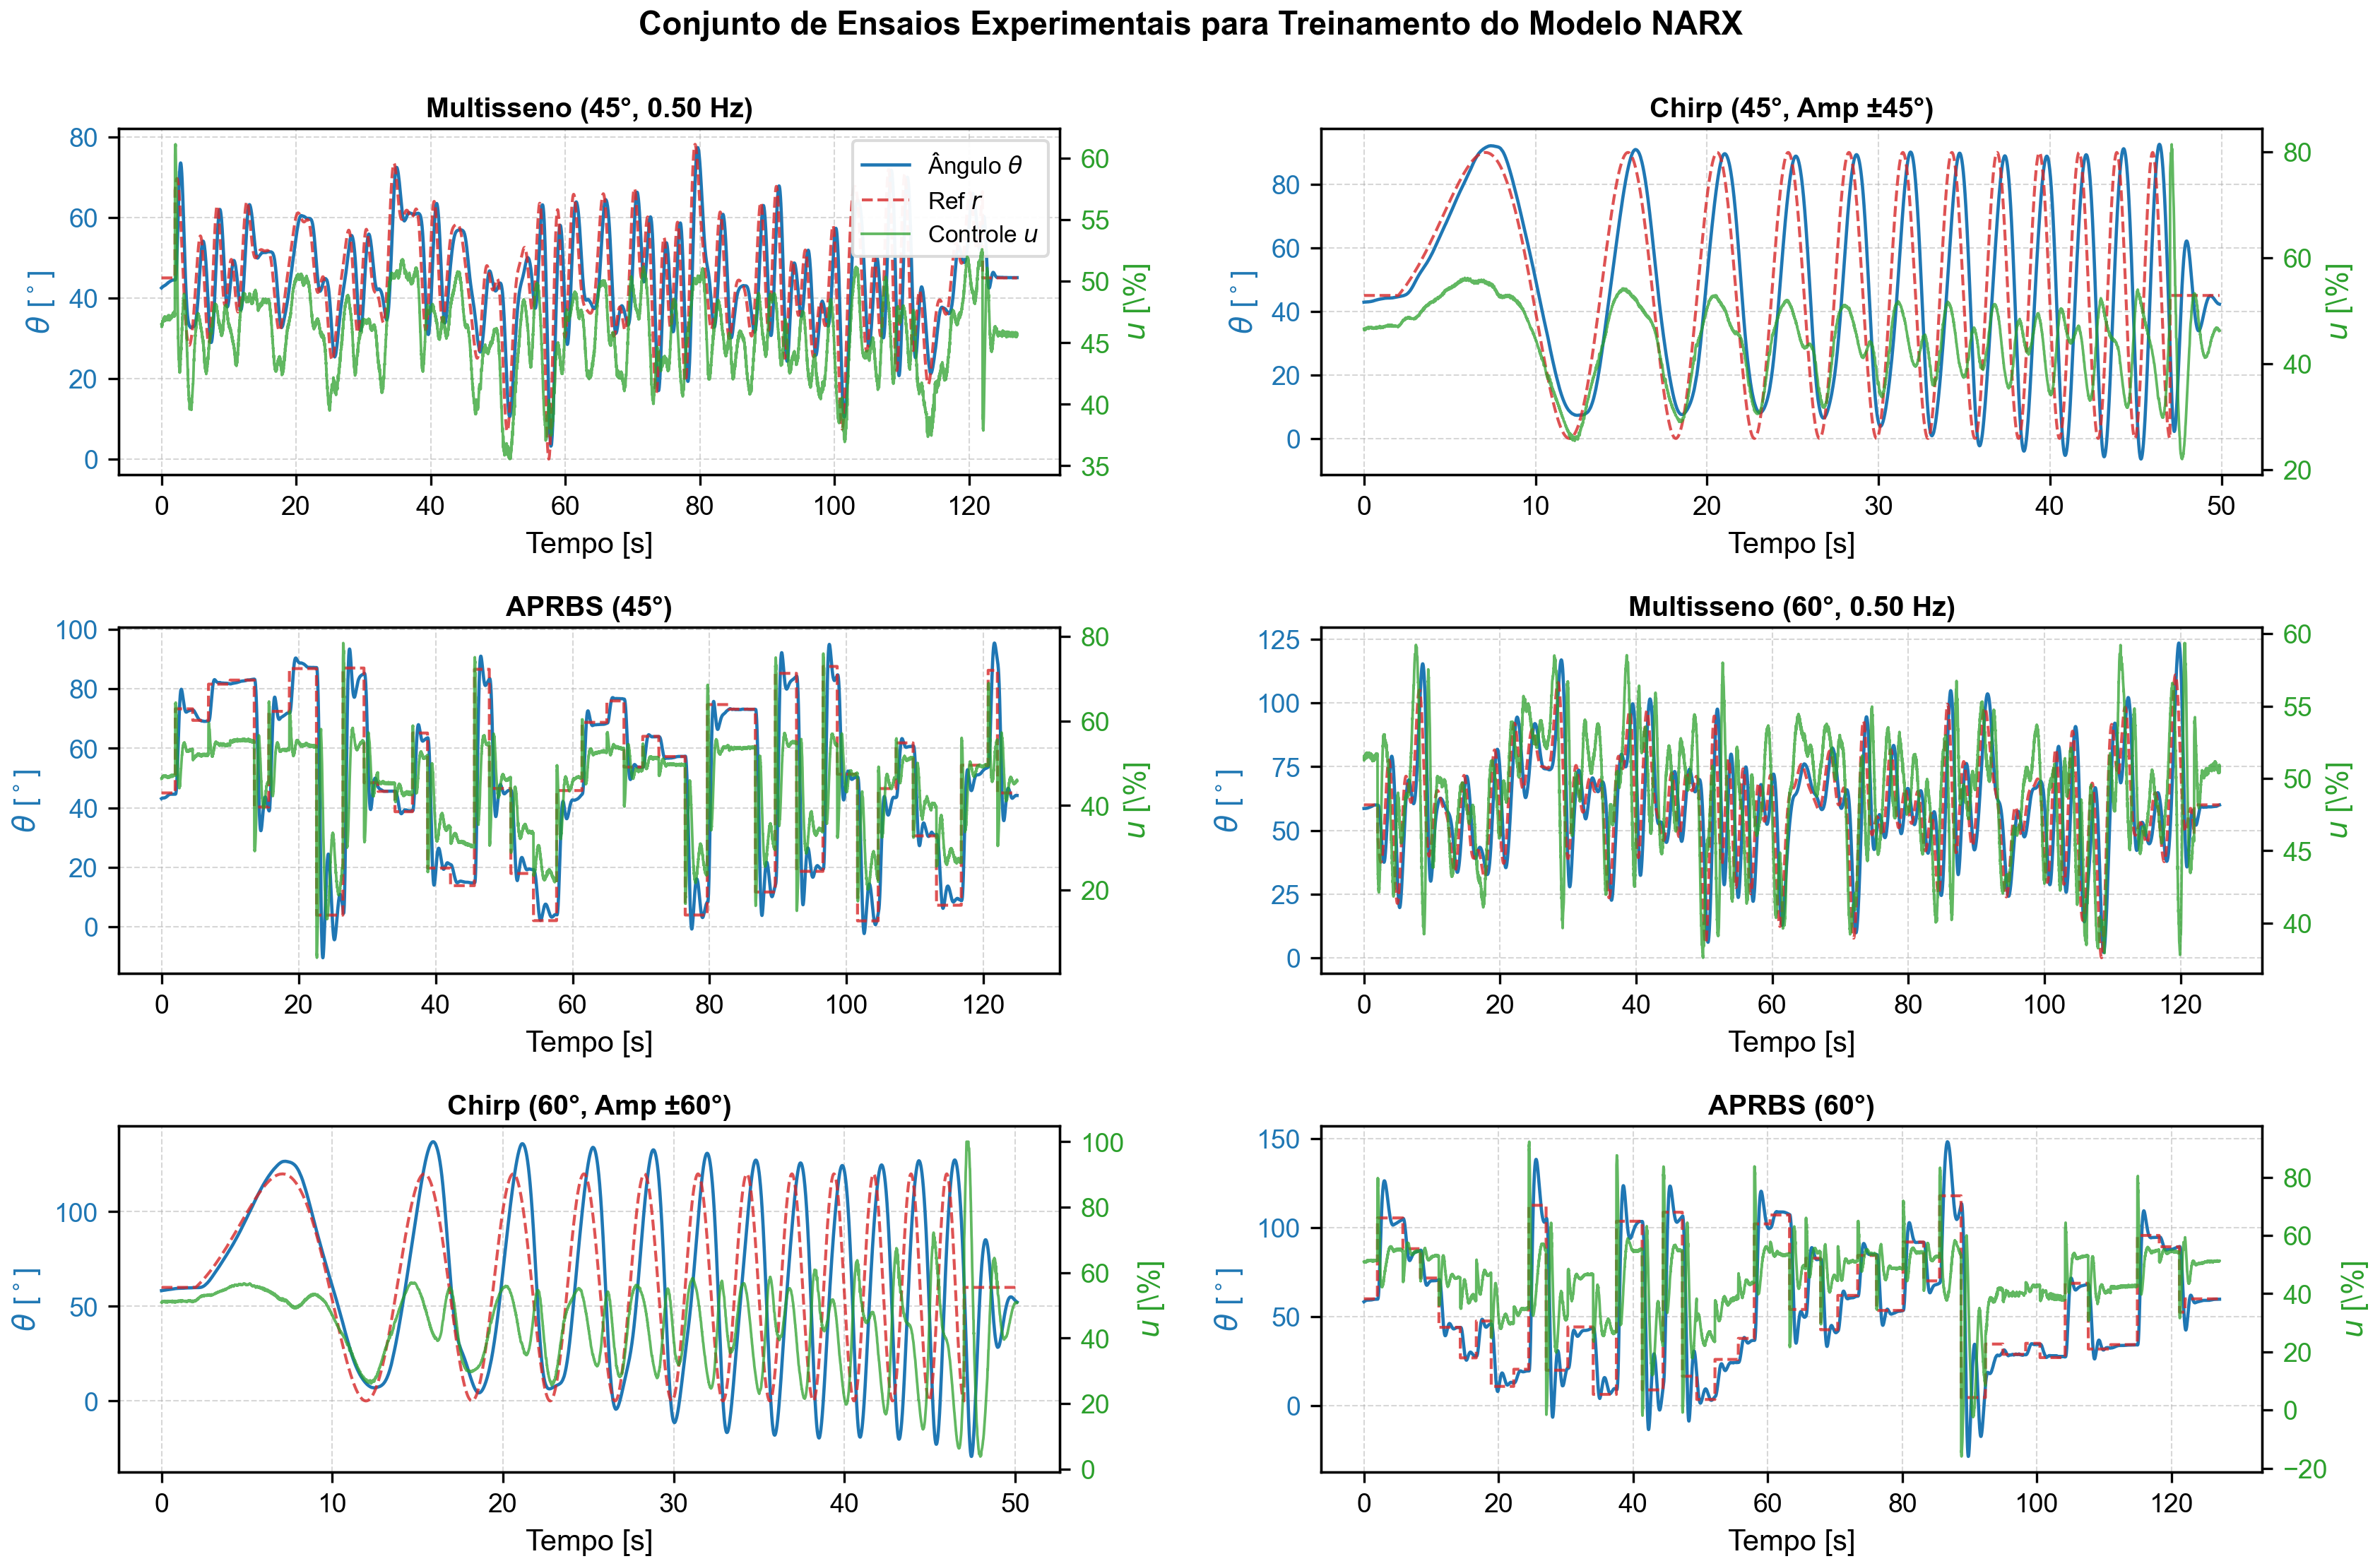
\includegraphics[width=0.90\textwidth]{img/resultados/narx_train_datasets.png}
    \sourceFig{o autor, 2026.}
\end{figure}

\begin{figure}[H]
    \centering
    \caption{Sinais de ensaios de validação independente.}
    \label{fig:sinais_validacao}
    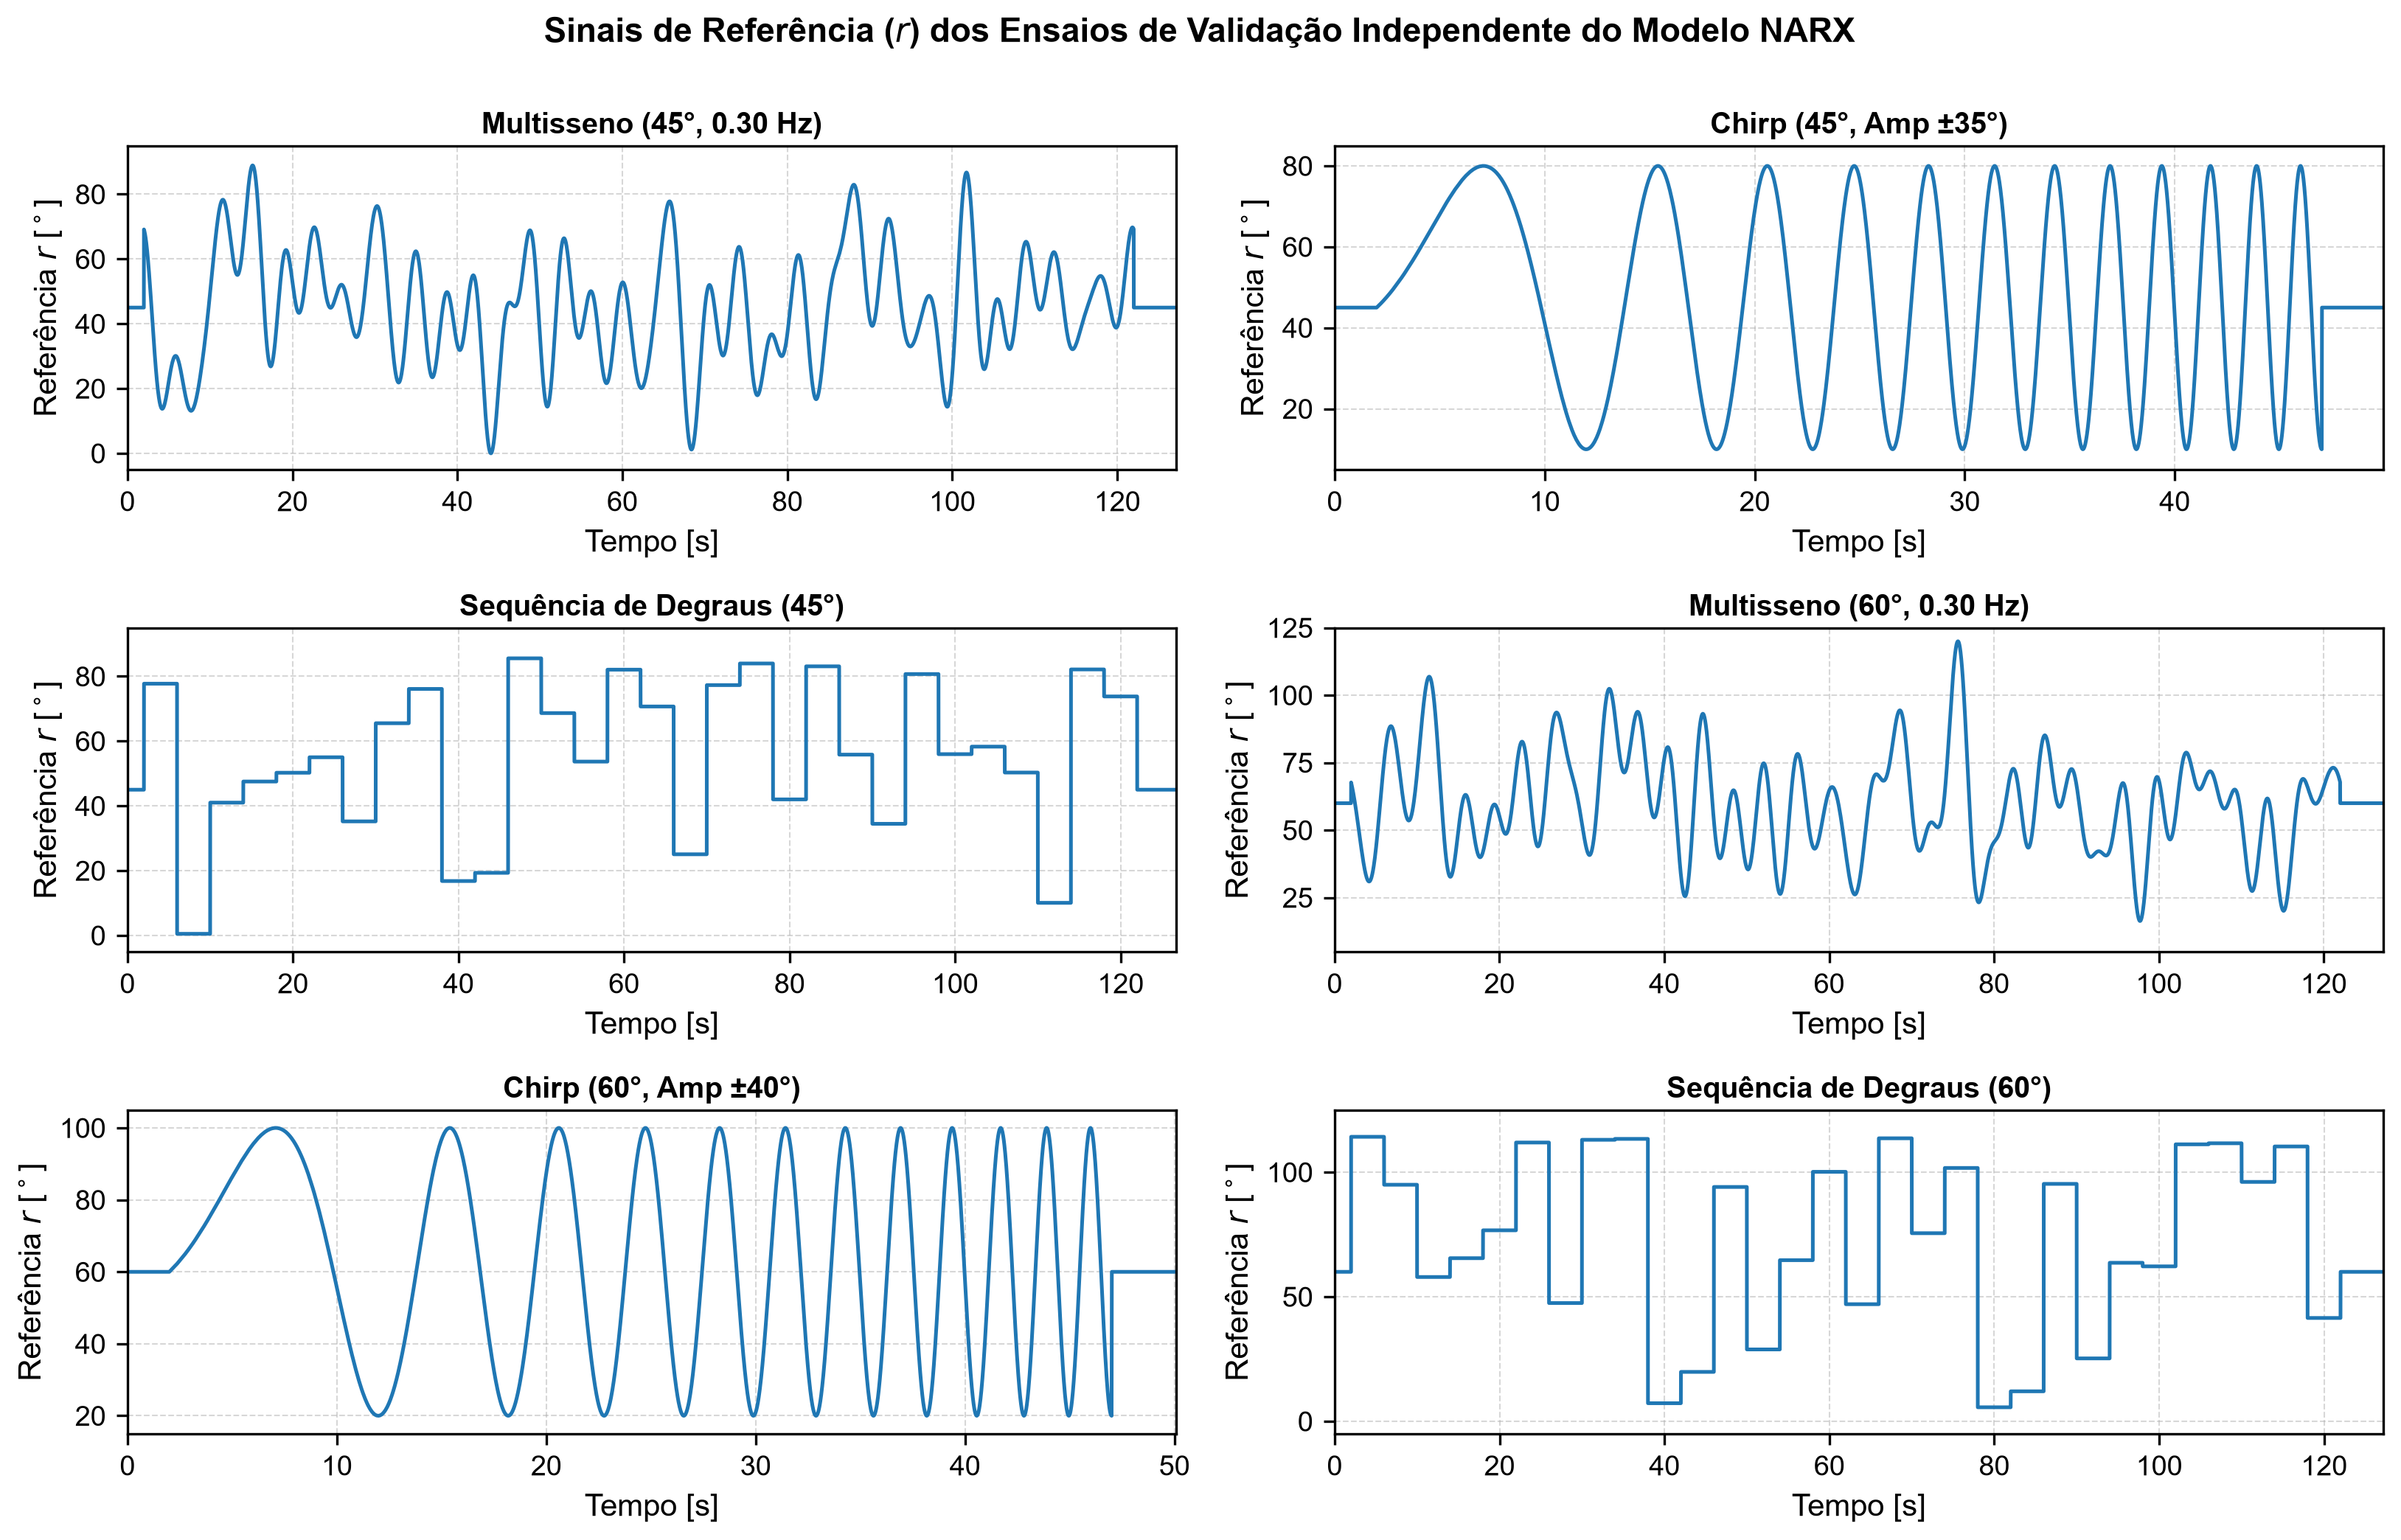
\includegraphics[width=0.90\textwidth]{img/resultados/narx_val_datasets.png}
    \sourceFig{o autor, 2026.}
\end{figure}

\subsubsection{Procedimento de Coleta de Dados}

Durante os ensaios, os dados foram transmitidos em tempo real pela interface USART2 do microcontrolador STM32 Nucleo-F446RE a uma taxa de comunicação de 500.000\,baud para o computador hospedeiro. Cada quadro de telemetria transmitido continha o carimbo de tempo determinístico (\textit{timestamp} com resolução de microssegundos), o sinal de referência $r(t)$, a ação de controle de saída $u(t)$ calculada pelo PID (expressa em porcentagem de \textit{duty cycle} do PWM no ESC) e o ângulo $\theta(t)$ estimado pelo filtro complementar a partir dos eixos do acelerômetro e giroscópio.

Os pacotes seriais foram capturados por um script Python dedicado utilizando a biblioteca \texttt{pyserial}, armazenados em arquivos estruturados de formato CSV e submetidos à rotina de pré-processamento, na qual os primeiros 10\,s (partida do motor e acomodação da comunicação) e os últimos 13\,s (desativação e frenagem) foram aparados, preservando os trechos estacionários de regime contínuo. O Algoritmo~\ref{alg:aquisicao_dados} sintetiza a lógica do laço em tempo real executada no microcontrolador durante as coletas.

\begin{algorithm}[H]
\caption{Ciclo Determinístico de Amostragem e Telemetria no STM32}
\begin{algorithmic}[1]
\label{alg:aquisicao_dados}
\Procedure{Setup}{}
    \State Inicializar periféricos (TIM, I$^2$C no modo Fast 400\,kHz, UART a 500\,kbaud, PWM a 50\,Hz)
    \State Calibrar offsets de bias do giroscópio da IMU ICM-20948 em repouso
    \State Inicializar estados internos do filtro complementar e integrador do PID
\EndProcedure

\Statex
\Procedure{Loop Amostragem Determinística}{}
    \State Aguardar comando de sincronização de ensaio via UART
    \State $t_{\text{inicio}} \gets \text{obterMicros()}$

    \While{$\text{ensaioAtivo}$}
        \State Sincronizar com período base do Timer de hardware ($T_s = 10\,\text{ms} \to 100\,\text{Hz}$)
        \State $t_{\text{atual}} \gets \text{obterMicros()} - t_{\text{inicio}}$

        \State Atualizar referência angular dinâmica: $\theta_{\text{ref}} \gets \text{avaliarSinalExcitacao}(t_{\text{atual}})$
        \State Ler acelerômetro ($a_x, a_z$) e giroscópio ($\omega_y$) da IMU via I$^2$C DMA
        \State Estimar ângulo atual $\theta(k)$ via filtro complementar de fusão sensorial
        \State Calcular esforço de controle $u(k) \gets \text{PID}(\theta_{\text{ref}},\, \theta(k))$ com saturação $[0,\, 100]\%$
        \State Atualizar comparador de captura do Timer de PWM para o ESC
        \State Enviar pacote binário de telemetria $(t_{\text{atual}},\, \theta(k),\, \theta_{\text{ref}},\, u(k))$ via UART DMA
    \EndWhile

    \State Desativar propulsão ($u \gets 0\%$) e aguardar parada mecânica
\EndProcedure
\end{algorithmic}
\end{algorithm}

% ------------------------------------------------------------
\subsection{Modelo NARX e Algoritmo FROLS}
\label{subsec:narx_frols}

Embora as equações diferenciais da física clássica~\eqref{eq:dinamica} forneçam a base teórica sobre as forças atuantes, sua parametrização experimental revelou limitações práticas: o modelo analítico simplificado não conseguiu se ajustar com fidelidade às dinâmicas reais da bancada (como o atrito seco dos mancais e as perdas aerodinâmicas do conjunto motor). Em contrapartida, a representação discreta orientada a dados via modelo NARX (\textit{Nonlinear AutoRegressive with eXogenous inputs}) apresentou convergência imediata e excelente aderência aos ensaios experimentais logo na primeira identificação. Por capturar com precisão a dinâmica não-linear de fase e amplitude sem exigir a integração contínua de equações diferenciais, o modelo NARX foi a formulação adotada para sintetizar o preditor utilizado no NMPC e na validação em \textit{Software-in-the-Loop} (SIL).


O modelo NARX polinomial discreto de entrada e saída única (SISO) mapeia a predição da saída angular futura $\hat{y}(k)$ como uma função polinomial expansível de saídas passadas e entradas passadas:
\begin{equation}
    \hat{y}(k) = F\!\left(y(k-1),\,\ldots,\,y(k-n_y),\; u(k-1),\,\ldots,\,u(k-n_u)\right),
    \label{eq:narx_geral}
\end{equation}
\noindent onde $n_y$ e $n_u$ são as ordens de atraso temporal na saída e na entrada, respectivamente. A representação linear-nos-parâmetros assume a forma:
\begin{equation}
    \hat{y}(k) = \sum_{m=1}^{M} \theta_m p_m(k),
    \label{eq:narx_linear_parametros}
\end{equation}
\noindent em que $p_m(k)$ são os monômios ou regressores formados por combinações de potências e produtos cruzados dos termos autorregressivos $y(k-i)$ e exógenos $u(k-j)$ até um grau de não-linearidade polinomial $\ell$, $\theta_m$ são os coeficientes constantes a estimar e $M$ denota o número total de regressores candidatos.

Para a planta do aeropêndulo operando a $100$\,Hz, os hiperparâmetros estruturais candidatos foram definidos como:
\begin{itemize}
    \item Ordem de memória de saída: $n_y = 15$ ($150$\,ms de histórico temporal);
    \item Ordem de memória de entrada: $n_u = 15$ ($150$\,ms de histórico de comandos);
    \item Grau polinomial de não-linearidade: $\ell = 2$ (termos lineares, produtos cruzados e termos quadráticos puros).
\end{itemize}

O número total de regressores candidatos gerados pela combinação combinatória é dado por:
\begin{equation}
    M_{\text{total}} = \frac{(n_y + n_u + \ell)!}{(n_y + n_u)!\,\ell!} = \frac{(15 + 15 + 2)!}{30!\,2!} = \frac{32 \times 31}{2} = 496 \text{ termos},
\end{equation}
\noindent subdivididos em 1 termo constante, 30 termos lineares de primeira ordem e 465 termos quadráticos de segunda ordem.

Estimar todos os 496 coeficientes simultaneamente induziria forte multicolinearidade, sobreparametrização numérica e instabilidade dinâmica em simulação recursiva livre. Por conseguinte, aplicou-se o algoritmo FROLS (\textit{Forward Regression Orthogonal Least Squares}) baseado no critério da Razão de Redução do Erro, ERR (\textit{Error Reduction Ratio}) \cite{chen1989}.

O algoritmo FROLS transforma iterativamente o conjunto de regressores candidatos correlacionados $P = [p_1, \ldots, p_M]$ em um conjunto de bases ortogonais $W = [w_1, \ldots, w_M]$ por decomposição matricial clássica:
\begin{equation}
    P = W A,
\end{equation}
\noindent onde $A$ é uma matriz triangular superior com diagonal unitária. O critério ERR de cada regressor candidato $p_m$ no passo $i$ de seleção é definido pela fração da variância total da saída explicada pela inclusão desse termo:
\begin{equation}
    [\text{ERR}]_i = \frac{g_i^2 \, w_i^\top w_i}{y^\top y} \times 100\%, \qquad g_i = \frac{w_i^\top y}{w_i^\top w_i}.
    \label{eq:err_criterio}
\end{equation}

A cada iteração, o algoritmo seleciona avidamente (\textit{greedy selection}) o regressor que fornece a maior contribuição $[\text{ERR}]_i$. O processo de seleção é interrompido quando a redução adicional de erro atinge um limiar desprezível ou quando se atinge o número pré-fixado de regressores parcimoniosos. No projeto, estipulou-se a seleção estrita de $10$ termos (\texttt{n\_components = 10}), garantindo que o modelo resultante seja compacto, computacionalmente eficiente para o resolvedor IPOPT do NMPC e numericamente estável.

\subsubsection{Avaliação em Simulação Livre}

A validação de modelos NARX polinomiais não pode ser fundamentada apenas no erro de predição um-passo-à-frente, OSA (\textit{One-Step-Ahead}), pois nessa modalidade a realimentação contínua do estado medido $y(k-1)$ mascara eventuais instabilidades intrínsecas e erros acumulados de ganho. Para qualificar o modelo preditivo que subsidiará o NMPC, a validação foi conduzida exclusivamente por meio de simulação livre, FR (\textit{Free-Run}):
\begin{equation}
    \hat{y}_{\text{FR}}(k) = F\!\left(\hat{y}_{\text{FR}}(k-1),\,\ldots,\,\hat{y}_{\text{FR}}(k-n_y),\; u(k-1),\,\ldots,\,u(k-n_u)\right),
\end{equation}
\noindent em que, após a inicialização com as condições iniciais nos primeiros $n_y$ instantes, todas as saídas subsequentes são geradas de maneira estritamente autorregressiva utilizando apenas suas próprias estimativas passadas $\hat{y}_{\text{FR}}$ e a sequência de controle real $u$.

A aderência quantitativa do modelo é avaliada por três métricas consolidadas sobre os dados de validação retidos:
\begin{align}
    \text{RMSE} &= \sqrt{\frac{1}{N} \sum_{k=1}^{N} \bigl(y(k) - \hat{y}(k)\bigr)^2}, \label{eq:rmse} \\
    \text{MAE}  &= \frac{1}{N} \sum_{k=1}^{N} \bigl|y(k) - \hat{y}(k)\bigr|, \label{eq:mae} \\
    \text{FIT}  &= \left(1 - \frac{\|y - \hat{y}\|_2}{\|y - \bar{y}\|_2}\right) \times 100\%, \label{eq:fit}
\end{align}
\noindent onde $y(k)$ é o ângulo experimental medido pela IMU, $\hat{y}(k)$ é a trajetória predita pelo modelo NARX e $\bar{y}$ é a média da saída experimental.

Complementarmente, a formulação contínua da Equação~\eqref{eq:estadonl} também foi parametrizada pelo método \textit{grey-box} não-linear via \textit{multiple shooting} com diferenciação automática em JAX \cite{helonayala_ms}, servindo como termo comparativo de sensibilidade física. Conforme demonstrado no Capítulo~\ref{cap:resultados}, o modelo polinomial NARX sobressai-se em fidelidade de fase e aderência estática quadrática ao longo de longos horizontes temporais, consolidando-se como a base preditiva oficial do sistema preditivo ótimo.
 
 
% ============================================================
\section{Síntese do Controlador}
\label{sec:sintese}
 
Esta seção descreve a síntese dos três controladores avaliados no projeto. O
controlador PID é sintetizado primeiro, pois desempenha papel duplo, ele estabiliza
a planta durante os ensaios de identificação em malha fechada e serve como
referência de desempenho na comparação final. Em seguida, o NMPC é formulado e
resolvido offline via CasADi, e sua política ótima é utilizada para gerar o
\textit{dataset} de treinamento da rede neural MLP.
 
% ------------------------------------------------------------
% ------------------------------------------------------------
\subsection{Controlador PID}
\label{sec:pid}

O controlador PID cumpre duas funções metodológicas no projeto: a de estabilizar o aeropêndulo em malha fechada durante os ensaios de varredura dinâmica para coleta de dados ricos de identificação (Seção~\ref{subsec:ensaios}) e a de servir como linha de base de desempenho linear clássico para a comparação final com o NMPC e a rede neural MLP embarcada.

\subsubsection{Linearização no Ponto de Operação}

Devido à natureza subamortecida e instável do aeropêndulo em malha aberta, a sintonia preliminar partiu de uma aproximação linear de segunda ordem em torno do ponto de operação nominal $\theta_0 = 40^\circ$. A linearização da dinâmica rotacional~\eqref{eq:dinamica} por expansão em série de Taylor de primeira ordem resulta na representação em espaço de estados incremental:
\begin{equation}
    \delta\dot{x} = A\,\delta x + B\,\delta u, \qquad \delta y = C\,\delta x,
    \label{eq:linear_eq}
\end{equation}
\noindent onde as matrizes Jacobianas avaliadas no ponto de equilíbrio $(\theta_0, u_0)$ fornecem a função de transferência contínua identificada a partir dos primeiros ensaios experimentais de degrau:
\begin{equation}
    G(s) = \frac{\Delta\theta(s)}{\Delta u(s)} = \frac{K\,\omega_n^2}{s^2 + 2\zeta\omega_n s + \omega_n^2} = \frac{6{,}9522}{s^2 + 0{,}8755\,s + 6{,}2537}.
    \label{eq:tf_continua}
\end{equation}

A análise dos polos de malha aberta revela as propriedades dinâmicas intrínsecas da planta na região de operação:
\begin{itemize}
    \item Frequência natural de oscilação: $\omega_n = \sqrt{6{,}2537} \approx 2{,}5007$\,rad/s ($f_n \approx 0{,}398$\,Hz);
    \item Coeficiente de amortecimento: $\zeta = \frac{0{,}8755}{2\omega_n} \approx 0{,}1751$ (planta severamente subamortecida);
    \item Ganho estático incremental: $K_{dc} = \frac{6{,}9522}{6{,}2537} \approx 1{,}1117^\circ/\%$.
\end{itemize}

Para a implantação computacional e simulação digital em tempo discreto com período de amostragem $T_s = 10$\,ms ($f_s = 100$\,Hz), a função de transferência contínua~\eqref{eq:tf_continua} foi discretizada pelo método do Segurador de Ordem Zero (\textit{Zero-Order Hold} - ZOH), resultando em:
\begin{equation}
    G(z) = \frac{0{,}0003466\,z^{-1} + 0{,}0003456\,z^{-2}}{1 - 1{,}9907\,z^{-1} + 0{,}9913\,z^{-2}},
    \label{eq:tf_discreta}
\end{equation}
\noindent que corresponde à equação recursiva a diferenças:
\begin{equation}
    y[k] = 1{,}9907\,y[k-1] - 0{,}9913\,y[k-2] + 0{,}0003466\,u[k-1] + 0{,}0003456\,u[k-2].
\end{equation}

\subsubsection{Sintonia em Frequência}

A determinação dos ganhos $K_p$, $K_i$ e $K_d$ foi conduzida no ambiente MATLAB utilizando técnicas de resposta em frequência, visando conciliar amortecimento do modo oscilatório com rapidez de resposta sem provocar saturações prematuras do atuador. Estabeleceram-se as seguintes especificações de malha fechada:
\begin{itemize}
    \item Sobressinal percentual máximo: $M_p = 15\%$;
    \item Tempo de acomodação ($2\%$): $t_s = 5{,}0$\,s;
    \item Fator de amortecimento de malha fechada:
    \begin{equation}
        \zeta_{mf} = \frac{-\ln(M_p/100)}{\sqrt{\pi^2 + \ln^2(M_p/100)}} = \frac{-\ln(0{,}15)}{\sqrt{\pi^2 + \ln^2(0{,}15)}} \approx 0{,}5169;
    \end{equation}
    \item Frequência natural desejada: $\omega_{n,mf} = \frac{4}{\zeta_{mf}\,t_s} \approx 1{,}5476$\,rad/s;
    \item Margem de fase especificada: $\text{PM} \approx 53{,}2^\circ$ na frequência de cruzamento de ganho $\omega_c \approx 1{,}50$\,rad/s.
\end{itemize}

A síntese computacional pelo algoritmo \texttt{pidtune} com refinamento experimental na bancada conduziu aos seguintes parâmetros finais de sintonia:
\begin{equation}
    K_p = 0{,}5793, \qquad K_i = 0{,}6647, \qquad K_d = 0{,}2000.
    \label{eq:ganhos_pid}
\end{equation}

\subsubsection{Implementação Digital no Firmware}

No microcontrolador STM32 Nucleo-F446RE, a lei de controle PID é executada de forma estritamente periódica a cada $T_s = 10$\,ms dentro da rotina de interrupção temporal. Para evitar o fenômeno destrutivo do \textit{derivative kick} (surtos de derivada provocados por transições abruptas no sinal de referência $r[k]$), a ação derivativa foi aplicada diretamente sobre a medição angular filtrada $y[k]$ fornecida pela IMU \cite{astrom1995}.

A discretização das parcelas de controle no instante $k$ obedece à formulação:
\begin{align}
    u_p[k] &= K_p\, e[k], \label{eq:pid_p} \\
    u_i[k] &= u_i[k-1] + K_i\,\frac{T_s}{2}\,\bigl(e[k] + e[k-1]\bigr), \label{eq:pid_i} \\
    u_d[k] &= -\frac{K_d}{T_s}\,\bigl(y[k] - y[k-1]\bigr), \label{eq:pid_d}
\end{align}
\noindent onde $e[k] = r[k] - y[k]$ denota o erro de rastreamento angular e a parcela integral~\eqref{eq:pid_i} utiliza a integração trapezoidal (transformada de Tustin) para minimizar a distorção de fase em relação à integração contínua.

A ação ideal $u_{\text{ideal}}[k] = u_p[k] + u_i[k] + u_d[k]$ é submetida aos limites de saturação do atuador:
\begin{equation}
    u[k] = \text{sat}\bigl(u_{\text{ideal}}[k],\; -u_{\max},\; u_{\max}\bigr), \qquad u_{\max} = 100\%,
\end{equation}
\noindent sendo convertida em largura de pulso para o ESC bidirecional através da relação linear:
\begin{equation}
    \text{Pulso PWM}\,[\mu\text{s}] = 1500 + 5 \times u[k].
\end{equation}

Para prevenir o fenômeno de \textit{integral windup} decorrente de saturações operacionais em manobras rápidas, implementou-se um mecanismo de anti-windup reativo por retrocálculo (\textit{back-calculation}):
\begin{equation}
    u_i[k] \leftarrow u_i[k] - \bigl(u_{\text{ideal}}[k] - u[k]\bigr).
    \label{eq:anti_windup}
\end{equation}
Esse mecanismo descarrega instantaneamente o integrador digital na proporção exata da saturação sofrida, assegurando retorno imediato à região linear assim que o sinal de erro se inverte.

\subsubsection{Validação Experimental em Degraus}

A validação da malha PID foi conduzida na bancada física por meio de degraus de referência em três pontos de operação: $30^\circ$, $40^\circ$ (ponto nominal de sintonia) e $60^\circ$. A Figura~\ref{fig:pid_degraus_consolidado} apresenta o confronto direto entre a simulação do modelo linear discretizado~\eqref{eq:tf_discreta} e a resposta experimental real registrada pela telemetria serial a 100\,Hz.

\begin{figure}[H]
    \centering
    \caption{Resposta ao degrau do controlador PID}
    \label{fig:pid_degraus_consolidado}
    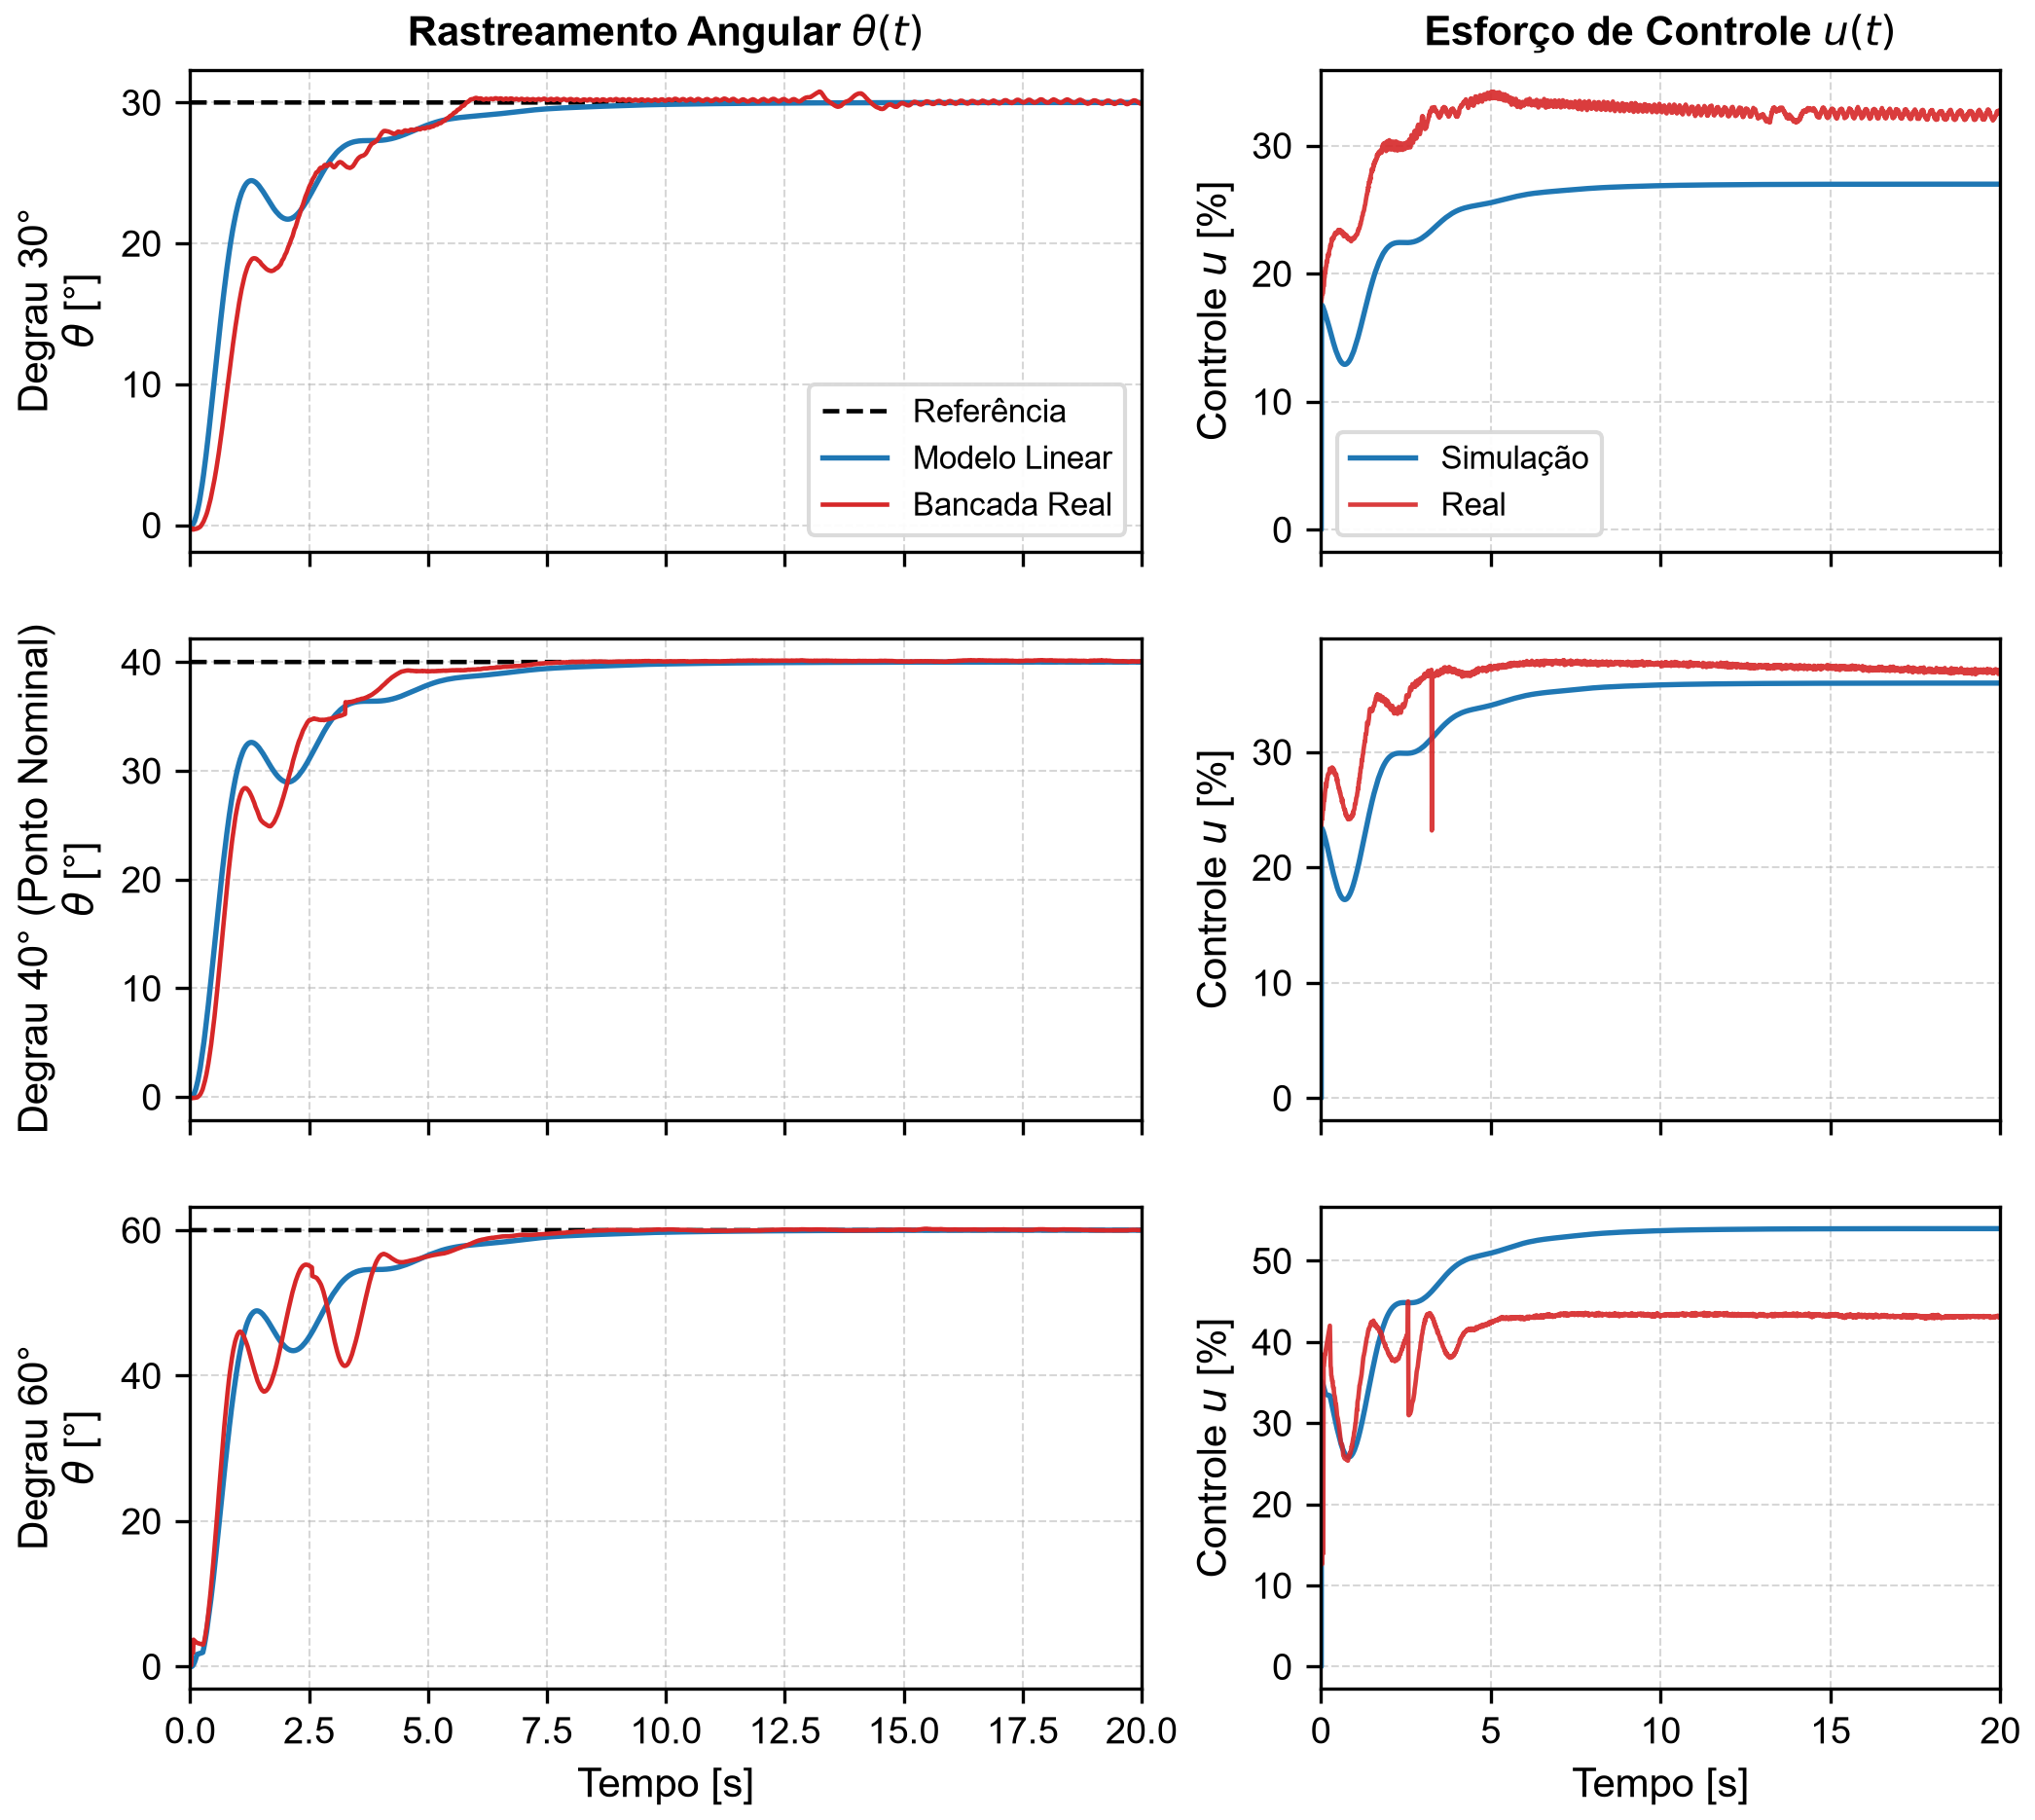
\includegraphics[width=0.95\textwidth]{img/pid_degraus_consolidado.png}
    \sourceFig{o autor, 2026.}
\end{figure}

A análise comparativa da Figura~\ref{fig:pid_degraus_consolidado} revela aspectos fundamentais da dinâmica do aeropêndulo:
\begin{itemize}
    \item \textbf{Ponto Nominal ($40^\circ$):} No patamar em torno do qual o modelo linear foi sintonizado, observa-se alta concordância entre a resposta simulada e a real. O erro transitório de modelagem permanece inferior a $\pm 6^\circ$ durante a subida, atingindo regime permanente em torno de 5\,s com erro estacionário nulo e esforço de controle praticamente idêntico ($u_{\text{sim}} = 35{,}98\%$ contra $u_{\text{real}} = 36{,}83\%$);
    
    \item \textbf{Assimetria e Variação de Ganho Estático ($30^\circ$ e $60^\circ$):} À medida que a referência se afasta do ponto nominal, manifesta-se a severa não-linearidade da planta. Em $30^\circ$, o empuxo contínuo exigido para equilíbrio é de $32{,}61\%$, enquanto o modelo linear prediz $26{,}98\%$ (discrepância de $5{,}63\%$ de duty cycle). Em $60^\circ$, onde a componente gravitacional restauradora $(m_1 L_1 - m_2 L_2)g\sin(\theta)$ impõe máxima resistência, o esforço real exigido atinge $42{,}74\%$, divergindo dos $53{,}97\%$ calculados linearmente (erro de ganho estático superior a $11\%$ de duty cycle);
    
    \item \textbf{Diferenças de Dinâmica Transitória:} A resposta real em $60^\circ$ apresenta amortecimento superior ao previsto pelo modelo linear em virtude do aumento do arrasto aerodinâmico induzido pela hélice em altas rotações.
\end{itemize}

Essa disparidade comprova experimentalmente que um modelo linear invariante no tempo e um controlador linear clássico (PID) são incapazes de garantir desempenho homogêneo ao longo de todo o envelope de voo do aeropêndulo. Esse resultado justifica plenamente a necessidade de adotar uma formulação preditiva não-linear (NMPC) baseada em modelo dinâmico NARX, apresentada a seguir.
% ------------------------------------------------------------
\subsection{Formulação do NMPC}
\label{subsec:nmpc_ocp}

O NMPC fundamenta-se na resolução repetida, a cada período de amostragem $T_s$, de um Problema de Controle Ótimo (OCP) em horizonte finito \cite{rawlings2017}. A síntese offline desse controlador exige ferramentas capazes de (i)~expressar simbolicamente o modelo dinâmico não-linear, (ii)~transcrever o OCP em um Problema de Programação Não-Linear (NLP) e (iii)~calcular automaticamente as derivadas de primeira e segunda ordem exigidas pelo resolvedor numérico. O framework CasADi atende a esses três requisitos de forma integrada \cite{andersson2019}.

\subsubsection*{Problema de Controle Ótimo em Horizonte Finito}

Para o estado atual $x_k$ e a referência $x_{ref,k} = [\theta_{ref,k},\; 0]^\top$, define-se o conjunto de sequências de controle admissíveis
\begin{equation}
    \mathcal{U}_N(x_k) := \bigl\{U_k \mid
        (x_{k+j|k},\, u_{k+j}) \in \mathcal{Z},\;
        x_{k+N|k} \in \mathcal{X}_f,\;
        j = 0,\ldots,N-1
    \bigr\},
    \label{eq:admissivel}
\end{equation}
\noindent onde $\mathcal{Z} := \mathcal{X} \times \mathcal{U}$ é o conjunto admissível de pares estado-controle e $\mathcal{X}_f \subseteq \mathcal{X}$ é o conjunto terminal. O domínio de factibilidade do OCP é
\begin{equation}
    \mathcal{X}_N := \bigl\{x \in \mathcal{X} \mid
        \mathcal{U}_N(x) \neq \emptyset \bigr\},
    \label{eq:factivel}
\end{equation}
\noindent ou seja, o conjunto de estados a partir dos quais existe ao menos uma sequência de controle que satisfaz todas as restrições e conduz o sistema ao conjunto terminal em $N$ passos \cite{rawlings2017}.

O OCP resolvido no instante $k$ é
\begin{equation}
    \min_{U_k}\;
    \underbrace{\sum_{j=0}^{N-1}
    \ell\!\left(x_{k+j|k},\, u_{k+j},\, x_{ref,k}\right)}_{\text{custo acumulado}}
    +\;
    \underbrace{V_f\!\left(x_{k+N|k},\, x_{ref,k}\right)}_{\text{custo terminal}}
    \label{eq:ocp}
\end{equation}
\noindent sujeito a
\begin{align}
    x_{k+j+1|k} &= x_{k+j|k} + T_s\, f\!\left(x_{k+j|k},\, u_{k+j}\right),
    && j = 0, \ldots, N-1, \label{eq:ocp_dinamica} \\
    x_{k|k}      &= x_k, \label{eq:ocp_ic} \\
    u_{k+j}      &\in \mathcal{U}, && j = 0, \ldots, N-1, \label{eq:ocp_u} \\
    x_{k+j|k}    &\in \mathcal{X}, && j = 1, \ldots, N, \label{eq:ocp_x} \\
    x_{k+N|k}    &\in \mathcal{X}_f, \label{eq:ocp_terminal}
\end{align}
\noindent onde $N$ é o horizonte de predição; $U_k = \{u_{k}, \ldots, u_{k+N-1}\}$ é a sequência de controle a otimizar; $x_{k+j|k}$ é o estado predito $j$ passos à frente, propagado pela discretização de Euler explícita da dinâmica contínua~\eqref{eq:estadonl}; e $\mathcal{U}$ e $\mathcal{X}$ são os conjuntos admissíveis de entrada e de estado.

\subsubsection*{Custo de Estágio e Custo Terminal}

O custo de estágio adota a forma quadrática em relação ao vetor de estados completo $x = [\theta,\; \dot{\theta}]^\top$ e ao vetor de referência $x_{ref} = [\theta_{ref},\; 0]^\top$:
\begin{equation}
    \ell(x, u, x_{ref}) =
    (x - x_{ref})^\top Q\,(x - x_{ref}) + u^\top R\, u,
    \label{eq:custo_estagio}
\end{equation}
\noindent onde $Q \in \mathbb{R}^{2\times2}$ e $R \in \mathbb{R}$ são, respectivamente, as matrizes de peso definidas positivas ($Q \succ 0$ e $R > 0$). A matriz $Q$ penaliza o erro de rastreamento angular e a velocidade angular, garantindo o amortecimento do sistema, enquanto $R$ penaliza o esforço de controle, inibindo variações bruscas no sinal enviado ao ESC. A positividade estrita de $Q$ e $R$ garante que $\ell(x, u, x_{ref}) \geq \alpha_1(|x - x_{ref}|)$ para alguma função de classe $\mathcal{K}_\infty$, condição necessária para que a função de valor ótimo $V_N^0(\cdot)$ admita uma cota inferior compatível com os requisitos de uma função de Lyapunov \cite{rawlings2017}.


O custo terminal é definido de forma análoga sobre o vetor de estados:
\begin{equation}
    V_f(x, x_{ref}) =
    (x - x_{ref})^\top P\,(x - x_{ref}),
    \label{eq:custo_terminal}
\end{equation}
\noindent onde a matriz $P \succ 0$ é obtida pela solução da equação de Lyapunov do sistema linearizado em torno do ponto de equilíbrio, operando sob uma lei de controle local estabilizante $u = K(x - x_{ref})$. Essa escolha garante que $V_f$ atue como uma Função de Lyapunov de Controle (CLF) local: para todo $x \in \mathcal{X}_f$, existe $u = Kx$ tal que
\begin{equation}
    V_f\!\left(f(x, u),\, x_{ref}\right) - V_f(x, x_{ref})
    \leq -\ell(x, u, x_{ref}),
    \label{eq:clf}
\end{equation}
\noindent condição denominada suposição básica de estabilidade por
\citeonline{rawlings2017}. O conjunto terminal
$\mathcal{X}_f$ é escolhido como um subconjunto compacto e invariante por
controle em torno de $\theta_{ref}$, tipicamente um subnível de $V_f$, de
modo que~\eqref{eq:clf} seja satisfeita para todo $x \in \mathcal{X}_f$.

\subsubsection*{Estratégia de Horizonte Deslizante e Viabilidade Recursiva}

A estratégia de horizonte deslizante (\textit{receding horizon}) aplica apenas a primeira ação ótima $u_k^* = u^0(0; x_k)$ da sequência $U_k^* = \arg\min \eqref{eq:ocp}$, descarta os demais elementos e resolve novamente o OCP no instante seguinte com o novo estado medido $x_{k+1}$, incorporando retroalimentação de forma natural \cite{mayne2000}. A lei de controle implícita resultante é
\begin{equation}
    \kappa_N(x_k) := u^0(0;\, x_k), \qquad x_k \in \mathcal{X}_N.
    \label{eq:lei_controle}
\end{equation}

Uma propriedade fundamental dessa estratégia é a viabilidade recursiva, se o OCP é factível para o estado inicial $x_0 \in \mathcal{X}_N$, então ele permanece factível para todos os estados subsequentes $x_k$ do sistema em malha fechada $x^+ = f(x,
\kappa_N(x))$, desde que $\mathcal{X}_f$ seja invariante por controle \cite{rawlings2017}. Isso garante que o controlador nunca encontra um estado para o qual não exista solução, evitando falhas em operação.
Sob as condições~\eqref{eq:clf}, pode-se mostrar que a função de valor ótimo satisfaz
\begin{equation}
    V_N^0\!\left(f(x, \kappa_N(x))\right) \leq V_N^0(x) - \ell(x,\kappa_N(x))
    \quad \forall x \in \mathcal{X}_N,
    \label{eq:descida}
\end{equation}
\noindent o que caracteriza $V_N^0(\cdot)$ como uma função de Lyapunov do sistema em malha fechada, assegurando estabilidade assintótica da origem (erro de rastreamento nulo) em $\mathcal{X}_N$ \cite{rawlings2017}.

O OCP~\eqref{eq:ocp}--\eqref{eq:ocp_terminal} é transcrito em um NLP e resolvido pelo CasADi \cite{andersson2019}, que constrói grafos de expressão simbólica (DAGs) e calcula automaticamente as derivadas de primeira e segunda ordem exigidas pelo resolvedor numérico IPOPT.

% ------------------------------------------------------------
\subsection{Geração do \textit{Dataset}}

A política de controle ótima gerada pelo NMPC em malha fechada é utilizada para compor o \textit{dataset} de treinamento da rede neural MLP, conforme o bloco central da fase offline na Figura~\ref{fig:diagrama-blocos-projeto}. Para cada instante de simulação, o OCP~\eqref{eq:ocp} é parametrizado pela referência corrente $\theta_{ref,k}$, e registra-se o par entrada-saída:
\begin{equation}
    \mathcal{D} = \bigl\{
        \bigl(x_k,\; u_k^*\bigr)
    \bigr\}_{k=1}^{M},
    \label{eq:dataset}
\end{equation}
\noindent onde $x_k \in \mathbb{R}^{130}$ denota o vetor de características composto pelas $n_y = 15$ saídas passadas da planta ($\theta_{k-1}, \dots, \theta_{k-15}$), pelas $n_u = 15$ ações de controle passadas ($u_{k-1}, \dots, u_{k-15}$) e pelos $N = 100$ passos de referência futura no horizonte de predição ($\theta_{\text{ref}, k}, \dots, \theta_{\text{ref}, k+N-1}$), e $u_k^* \in \mathbb{R}$ representa a ação de controle ótima obtida da solução do OCP em malha fechada.

A inclusão das referências futuras dota a rede neural da capacidade de visão antecipada (\textit{preview}), permitindo compensar preventivamente a inércia mecânica da planta, em harmonia com a formulação do OCP da Seção~\ref{subsec:nmpc_ocp}. Para alimentar a resolução offline do controlador ótimo e assegurar rica cobertura do espaço de estados, sintetizou-se uma trajetória multivariada com duração de 187\,s, combinando trechos senoidais harmônicos até $0{,}50$\,Hz com degraus de amplitude comutada que percorrem desde $12^\circ$ até $110^\circ$, cobrindo dinâmicas de transição e regimes estáticos ao longo de todo o envelope operacional \cite{karg2020}.

O \textit{dataset} é normalizado componente a componente para o intervalo $[-1, 1]$ antes do treinamento, procedimento padrão que melhora o condicionamento do problema de otimização do aprendizado e a convergência do algoritmo Adam \cite{karg2020}.

% ------------------------------------------------------------
\subsection{Arquitetura e Treinamento da MLP}

A implementação e o treinamento da rede neural MLP são realizados utilizando o PyTorch. O PyTorch é uma biblioteca de aprendizado de máquina que unifica facilidade de uso e alta performance computacional. Diferentemente de frameworks baseados na construção prévia de grafos estáticos de fluxo de dados, o PyTorch adota o paradigma de execução dinâmica e imperativa. Isso permite que os modelos de aprendizado profundo sejam programados e depurados como programas Python convencionais, mantendo o controle total do fluxo sob responsabilidade do usuário \cite{paszke2019}.
A estrutura da rede, a configuração dos hiperparâmetros e a rotina de otimização, que inclui um critério de parada prematura (\textit{early stopping}) para evitar \textit{overfitting}, estão consolidadas no Algoritmo~\ref{alg:treino_mlp}.

\begin{algorithm}
\caption{Treinamento da Rede Neural para Aproximação do Controlador}
\label{alg:treino_mlp}
\begin{algorithmic}[1]

\Procedure{TreinarAproximador}{}

    \State Carregar dataset gerado pelo controlador ótimo
    \State Dividir dataset em conjuntos de treino, validação e teste
    \State Inicializar rede neural e otimizador
    \State $melhorLoss \gets \infty$, \quad $contadorPaciencia \gets 0$

    \Statex
    \For{cada época}
        \State Atualizar pesos minimizando o erro nos batches de treino
        \State Avaliar erro no conjunto de validação

        \If{houve melhora na validação}
            \State Registrar melhora e salvar pesos atuais
            \State Resetar contador de paciência
        \Else
            \State Incrementar contador de paciência
            \If{paciência esgotada}
                \State \textbf{break} \Comment{\textit{Early stopping}}
            \EndIf
        \EndIf
    \EndFor

    \Statex
    \State Restaurar melhores pesos
    \State Avaliar desempenho final no conjunto de teste
    \State Exportar modelo para implantação embarcada

\EndProcedure
\end{algorithmic}
\end{algorithm}

% ============================================================
\section{Controle Embarcado em Tempo Real}
\label{sec:embarcado}

% ------------------------------------------------------------
\subsection{Conversão via X-CUBE-AI}

O STM32Cube.AI é uma ferramenta de software desenvolvida pela STMicroelectronics projetada para a implantação de aprendizado de máquina em microcontroladores (TinyML). Esse ecossistema atua como um gerador de código baseado em compilação, recebendo modelos treinados em plataformas como Keras e TensorFlow Lite para gerar código C otimizado para a linha de microcontroladores STM32 \cite{stmu2526}.

Diferentemente de abordagens baseadas em interpretadores embarcados, que processam a topologia do modelo em tempo de execução, a geração de código nativo pode aumentar consideravelmente o desempenho da inferência. Como apontado por \citeonline{david2021}, metodologias baseadas em compilação fixam as chamadas de operação diretamente em código de máquina, eliminando as etapas de roteamento do interpretador. A ferramenta analisa a topologia da rede neural, otimiza o uso de \textit{buffers} e mapeia as operações matemáticas diretamente para as capacidades de hardware do processador alvo, minimizando o uso de memória Flash e SRAM e permitindo a execução de inferências com restrições de latência e consumo energético.

% ------------------------------------------------------------
\subsection{Firmware de Controle no STM32}

O firmware de controle utiliza uma arquitetura orientada a eventos e não-bloqueante para garantir o atendimento ao \textit{deadline} de $T_s = 10$\,ms. Um temporizador de hardware (TIM) operando a 100\,Hz atua como base de tempo determinística. A cada disparo do timer, a CPU apenas inicia a transferência dos dados inerciais da IMU via I$^2$C utilizando acesso direto à memória (DMA) e retorna imediatamente do contexto de interrupção, não bloqueando a execução.

Apenas quando a transferência I$^2$C é concluída, uma interrupção de conclusão do DMA (\textit{Transfer Complete}) é acionada, desencadeando a rotina de controle principal. Neste momento, com os dados inerciais já disponíveis na memória SRAM, o processador realiza a leitura da referência angular, a estimação do estado atual via filtro complementar, a inferência da rede neural e a atualização do \textit{duty cycle} do PWM no ESC, conforme o Algoritmo~\ref{alg:isr_controle}.

As operações de ponto flutuante, em particular o cálculo de \texttt{atan2} no filtro complementar e as multiplicações matriciais da MLP gerada pelo X-CUBE-AI, são executadas nativamente pela FPU do Cortex-M4, eliminando a sobrecarga de emulação por software. A transmissão da telemetria ao final da rotina também é delegada a um canal DMA vinculado à UART. Essa delegação maciça da movimentação de dados aos periféricos garante que o tempo de CPU fique dedicado estritamente aos cálculos de controle.

\begin{algorithm}[H]
\caption{Rotina de Controle em Tempo Real (Arquitetura DMA)}
\label{alg:isr_controle}
\begin{algorithmic}[1]
\Statex \textbf{Base de Tempo:} $f_s = 100$\,Hz ($T_s = 10$\,ms)
\Statex

\Procedure{Timer\_ISR}{}
    \State \Comment{Disparo determinístico a cada 10ms}
    \State $\text{IniciarLeituraIMU\_DMA()}$ \Comment{Inicia transação I$^2$C em background}
\EndProcedure

\Statex
\Procedure{I2C\_DMA\_Complete\_ISR}{}
    \State \Comment{1. Leitura da Referência (UART)}
    \State $\theta_{ref} \gets \text{LerReferencia()}$

    \Statex
    \State \Comment{2. Estimação de Estados (FPU)}
    \State $\theta, \dot{\theta} \gets \text{EstimarEstados(Buffer\_I2C)}$

    \Statex
    \State \Comment{3. Cálculo da Ação de Controle (Inferência Neural)}
    \State $x_{\text{in}} \gets \text{MontarVetorEntrada}(\theta_{\text{hist}},\, u_{\text{hist}},\, r_{\text{futuro}})$ \Comment{130 variáveis com \textit{preview}}
    \State $u \gets \text{InferirMLP}(x_{\text{in}})$

    \Statex
    \State \Comment{4. Atuação (PWM)}
    \State $\text{AplicarControle}(u)$

    \Statex
    \State \Comment{5. Registro de Dados (UART DMA)}
    \State $\text{IniciarTelemetria\_DMA}(\theta,\; \dot{\theta},\; \theta_{ref},\; u)$
\EndProcedure
\end{algorithmic}
\end{algorithm}
% ============================================================

%----------------Cap_04----------------%
\chapter{Conclusão}
 
Este trabalho propôs e documentou o desenvolvimento de um controlador neural
embarcado que aproxima a política ótima de um Controle Preditivo Não-Linear
(NMPC) para rastreamento angular de um aeropêndulo instrumentado. A motivação
central reside na incompatibilidade entre o custo computacional da otimização
repetida do NMPC e os recursos disponíveis em microcontroladores de baixo custo,
problema recorrente em plataformas VTOL de pequeno porte.

Como referência de desempenho e como mecanismo de estabilização durante os
ensaios de identificação, um controlador PID foi sintonizado a partir do modelo
linearizado e implementado digitalmente com discretização trapezoidal e
anti-windup por \textit{back-calculation}. Os resultados preliminares da
Etapa~\ref{subsec:etapa2} confirmaram a não-linearidade do sistema, motivando o emprego do modelo não-linear para a síntese do NMPC.
 
A estratégia adotada é tecnicamente viável. Os três principais riscos identificados, divergência do modelo identificado, exaustão dos recursos de hardware e
instabilidade do controlador neural por dados fora da distribuição, possuem
ações preventivas e de contingência estabelecidas. A etapa de identificação (Etapa~\ref{subsec:etapa3})
encontra-se em andamento e as etapas subsequentes dependem diretamente da
qualidade do modelo obtido. Caso o critério de ajuste não seja satisfeito, a
estrutura do modelo será revisada antes de prosseguir. A compacidade da arquitetura
MLP e a quantização via X-CUBE-AI constituem caminhos de contingência caso
os limites de Flash e SRAM do STM32F446 sejam ultrapassados.
 
O cronograma prevê a conclusão da identificação e da síntese do NMPC no
primeiro semestre, reservando o segundo para o treinamento da rede, a implantação
embarcada e os ensaios experimentais comparativos. A comparação final entre PID,
NMPC e MLP embarcada, consolidada na Tabela~\ref{tab:comparacao_controladores},
constituirá a principal contribuição quantitativa do trabalho e permitirá avaliar
objetivamente os \textit{trade-offs} entre desempenho de rastreamento, rejeição a
perturbações e custo computacional em hardware embarcado de baixo custo.
 
%%----------------Cap_05----------------%
\chapter{Conclusão}
\label{cap:conclusao}

Este trabalho apresentou o projeto, a implementação e a validação experimental de uma arquitetura de controle preditivo neural embarcado (\textit{TinyML}), concebida para aproximar a política de um Controlador Preditivo Não-Linear (NMPC) ótimo e executá-la em tempo real em um microcontrolador de baixo custo para o rastreamento angular de um aeropêndulo instrumentado.

A motivação central da pesquisa fundamentou-se na superação do gargalo computacional associado à otimização numérica não-linear online: a resolução iterativa do problema de controle ótimo via resolvedores tradicionais (como o IPOPT no ambiente CasADi) exigiu tempos de convergência entre 90 e 460\,ms por ciclo de amostragem em computador de mesa. Diante de uma dinâmica mecatrônica rápida que impõe um período de controle de $T_s = 10$\,ms ($100$\,Hz), a transferência da inteligência preditiva para uma rede neural compacta em linguagem C viabilizou a execução em hardware embarcado com determinismo temporal estrito e elevada concordância dinâmica frente à lei ótima nominal.

% ============================================================
\section{Cumprimento dos Objetivos Específicos}
\label{sec:conclusao_objetivos}
% ============================================================

Os objetivos específicos propostos no Capítulo~\ref{cap:introducao} foram cumpridos nas seguintes etapas do desenvolvimento:

\begin{enumerate}
    \item \textbf{Síntese do Controlador PID Linear e Estabilização para Coleta de Dados:} Projetou-se e sintonizou-se um controlador PID clássico na bancada experimental. O controlador desempenhou papel duplo fundamental: garantiu a estabilização da planta em malha fechada durante os ensaios de varredura dinâmica em torno dos equilíbrios operacionais de $45^\circ$ e $60^\circ$, viabilizando a coleta de dados experimentais ricos em amplitude e frequência sem perda de estabilidade, e serviu como linha de base de desempenho linear para a comparação final.
    
    \item \textbf{Identificação Paramétrica do Modelo Dinâmico do Aeropêndulo:} A dinâmica da planta foi identificada por meio do algoritmo FROLS na formulação polinomial NARX, selecionando uma estrutura parcimoniosa de apenas 10 termos a partir de 496 regressores candidatos. O modelo demonstrou estabilidade estrutural e concordância de fase em simulação livre (\textit{free-run}) de longo horizonte. 
    
    \item \textbf{Formulação e Resolução Offline do Problema de Controle Ótimo (NMPC):} O NMPC foi estruturado no ambiente CasADi considerando o modelo preditivo não-linear, restrições operacionais nos atuadores ($0 \le u \le 80\%$) e penalização de esforço e variação de controle ($\Delta u$). A simulação confirmou que o custo computacional de resolução online é incompatível com a taxa de 100\,Hz do sistema mecatrônico, justificando a geração de uma base abrangente de trajetórias ótimas com horizonte de visão antecipada (\textit{preview}) para o aprendizado supervisionado.
    
    \item \textbf{Treinamento da Rede MLP e Implantação em Hardware Embarcado:} A rede neural do tipo MLP ($130 \to 128 \to 128 \to 1$) foi treinada supervisionadamente, alcançando coeficiente de determinação $R^2 = 0{,}999$ e aprendendo a compensar preventivamente a inércia mecânica. A implementação nativa em linguagem C com instruções de ponto flutuante na FPU Cortex-M4 operando a 180\,MHz alcançou tempo de inferência determinístico em torno de 2,07\,ms a 2,08\,ms, consumindo cerca de $20{,}7\%$ da janela de 10\,ms e garantindo uma folga de CPU de $79{,}3\%$. Adicionalmente, a exploração do framework ST X-CUBE-AI com compressão avançada demonstrou a possibilidade de reduzir em $86{,}4\%$ o consumo de memória Flash dos pesos, mantendo o comportamento em malha fechada praticamente indistinguível.
    
    \item \textbf{Comparação Experimental entre Controladores e Fechamento do Gap Sim-to-Real:} Os ensaios espelhados na bancada física frente aos sinais evidenciaram vantagens expressivas da compensação preditiva neural sobre o PID clássico, com redução de erro quadrático médio de rastreamento entre $69\%$ e $81\%$ em manobras agressivas de alta frequência e amplitude. Concomitantemente, a transição para a bancada revelou o viés estacionário e o travamento mecânico por atrito estático de rolamento (\textit{stick-slip}) decorrentes da ausência de ação integradora na MLP pura; a introdução da arquitetura híbrida (MLP com integrador residual paralelo saturado) atenuou o viés em mais de $96\%$ e reduziu o erro senoidal pela metade, fechando eficazmente o \textit{Sim-to-Real gap}.
\end{enumerate}

% ============================================================
\section{Sustentabilidade e Eficiência Energética}
\label{sec:conclusao_sustentabilidade}
% ============================================================

Em consonância com as diretrizes de projeto de engenharia, a solução desenvolvida apresenta impactos positivos diretos sobre eficiência energética e sustentabilidade:

\begin{itemize}
    \item \textbf{Eficiência Computacional e Redução de Consumo Elétrico:} A substituição do solucionador numérico iterativo NMPC (que exige computadores de alto desempenho com consumo típico entre 45\,W e 120\,W) pela inferência de redes neurais em microcontrolador ARM Cortex-M4 permite operar o sistema preditivo com consumo elétrico inferior a 0,5\,W. Essa redução de ordens de magnitude na potência computacional prolonga a autonomia de baterias em veículos não tripulados e viabiliza plataformas móveis energeticamente eficientes.
    \item \textbf{Otimização do Ciclo de Vida de Baterias:} O rastreamento angular mais suave e a atenuação de sobre-sinais (\textit{overshoots}) propiciados pela característica preditiva reduzem picos transitórios de corrente no motor elétrico BLDC, mitigando o estresse eletroquímico e térmico das baterias de polímero de lítio (LiPo) e estendendo sua vida útil operacional.
    \item \textbf{Reaproveitamento de Hardware e Baixo Impacto Material:} O projeto foi concebido sobre uma plataforma de desenvolvimento de baixo custo (STM32 Nucleo-F446RE) e reaproveitou integralmente a estrutura mecatrônica pré-existente da bancada, minimizando o descarte de componentes eletrônicos e o impacto ambiental por geração de lixo eletrônico.
\end{itemize}

% ============================================================
\section{Limitações do Trabalho}
\label{sec:conclusao_limitacoes}
% ============================================================

Embora os resultados experimentais atestem a viabilidade da metodologia desenvolvida, identificam-se aspectos limitantes que delimitam o escopo das conclusões obtidas:

\begin{enumerate}
    \item \textbf{Restrição a Planta com Um Único Grau de Liberdade (1-DOF):} A validação foi restrita ao movimento angular no plano vertical. Em plataformas aéreas completas (como quadrotores e veículos VTOL), manifestam-se acoplamentos inerciais e aerodinâmicos cruzados entre eixos (arfagem, rolamento e guinada), além de momentos giroscópicos decorrentes da variação de rotação de múltiplos motores, efeitos que demandam formulações multivariáveis mais complexas.
    
    \item \textbf{Dependência de Identificação Prévia em Malha Fechada:} A obtenção do modelo dinâmico NARX dependeu da existência prévia de um controlador estabilizador (PID linear) funcional na bancada. Em plantas instáveis em malha aberta para as quais não se dispõe de um controlador preliminar estável, a coleta de dados dinâmica exige metodologias alternativas de síntese ou identificação iterativa.
    
    \item \textbf{Sensibilidade a Discrepâncias Estáticas no Modelo Puramente por Dados:} A rede neural nominal opera como um aproximador de função estático baseado em dados. Discrepâncias entre a planta real e o modelo treinado (tais como perdas aerodinâmicas de recirculação em ângulos elevados e atrito seco de mancais) manifestaram-se como erros persistentes de regime permanente, tornando indispensável a adição de um integrador residual no firmware para assegurar erro estacionário nulo.
    
    \item \textbf{Sensibilidade à Variação de Tensão da Alimentação (Bateria LiPo):} Os parâmetros da rede neural foram sintetizados assumindo uma relação de empuxo constante. Em ensaios operacionais contínuos alimentados por baterias recarregáveis, a curva de descarga reduz a tensão de barramento e diminui o empuxo disponível para uma dada largura de pulso PWM. A rede neural estática não possui mecanismos intrínsecos de compensação para essa perda gradual de ganho do atuador.
    
\end{enumerate}

% ============================================================
\section{Trabalhos Futuros}
\label{sec:conclusao_futuros}
% ============================================================

Como desdobramentos desta pesquisa, sugerem-se as seguintes frentes de investigação:

\begin{enumerate}
    \item \textbf{Extensão para Sistemas com Múltiplos Graus de Liberdade (2-DOF e VTOL):} Aplicar a formulação de modelagem NARX multivariável e controle preditivo neural em bancadas biconduzidas (arfagem e guinada) e veículos aéreos VTOL em voo livre, avaliando o comportamento frente a perturbações atmosféricas e acoplamentos giroscópicos;
    
    \item \textbf{Quantização Inteira Pura em Ponto Fixo (INT8):} Investigar técnicas de quantização pós-treinamento e treinamento ciente de quantização (\textit{Quantization-Aware Training} - QAT) para representação inteira de 8 bits, permitindo a execução da política neural em microcontroladores ultracompactos (como núcleos ARM Cortex-M0+ ou Cortex-M33) desprovidos de unidade de ponto flutuante em hardware;
    
    \item \textbf{Mecanismos de Adaptação Paramétrica Online em Firmware:} Implementar esquemas adaptativos em tempo real, tais como estimadores recursivos de ganho de atuador baseados em Filtro de Kalman ou aprendizado por reforço residual, capazes de compensar a degradação de tensão da bateria e variações de carga útil ao longo do tempo de operação;
    
    \item \textbf{Certificação Formal de Estabilidade e Limites de Lipschitz:} Desenvolver métodos de análise baseados na constante de Lipschitz da rede treinada ou em funções de controle de barreira (\textit{Control Barrier Functions} - CBF) para delimitar o envelope seguro de operação do controlador neural embarcado.
\end{enumerate}

%--------------------ELEMENTOS PÓS-TEXTUAIS--------------------%

%\postextual

%--------------------Referências Bibliográficas--------------------%
\bibliography{bibliografia}

% Abra o arquivo postextual.tex para alterar os elementos pós-textuais de seu trabalho 
%% Este trabalho está licenciado sob a licença Creative Commons CC-BY-SA.
% Você é livre para usar, compartilhar e adaptar este material, desde que seja atribuída a autoria e que as obras derivadas mantenham a mesma licença.

%-----------------------------Apêndices-----------------------------%
\begin{apendicesenv}


\chapter{Tutorial de uso do modelo LaTeX de monografia/dissertação/tese PUCPR}
\label{apendice_tutorial}

Este modelo foi desenvolvido pelos professores Rayson Laroca e Jean Paul Barddal em \LaTeX, tomando como base um modelo de dissertação da Universidade Federal do Tocantins (UFT) estruturado com a classe \abnTeX.
Foram realizadas diversas adaptações para garantir sua conformidade com as normas para elaboração de trabalhos acadêmico-científicos da Pontifícia Universidade Católica do Paraná (PUCPR), que, por sua vez, seguem as diretrizes da Associação Brasileira de Normas Técnicas (ABNT).

\section*{1. Apresentação do Modelo}

Neste tutorial, será apresentada a estrutura básica do modelo a fim de facilitar sua utilização.
O modelo está disponível no seguinte endereço eletrônico: \url{https://www.overleaf.com/read/nqpnfkmqzhkb\#40fc88}.
Ao abrir o link em sua conta Overleaf, o usuário terá acesso a uma tela semelhante à mostrada na Figura\ref{fig:estrutura}.

\begin{figura}{0.9\textwidth}
    \caption{Modelo aberto no editor online Overleaf.}
    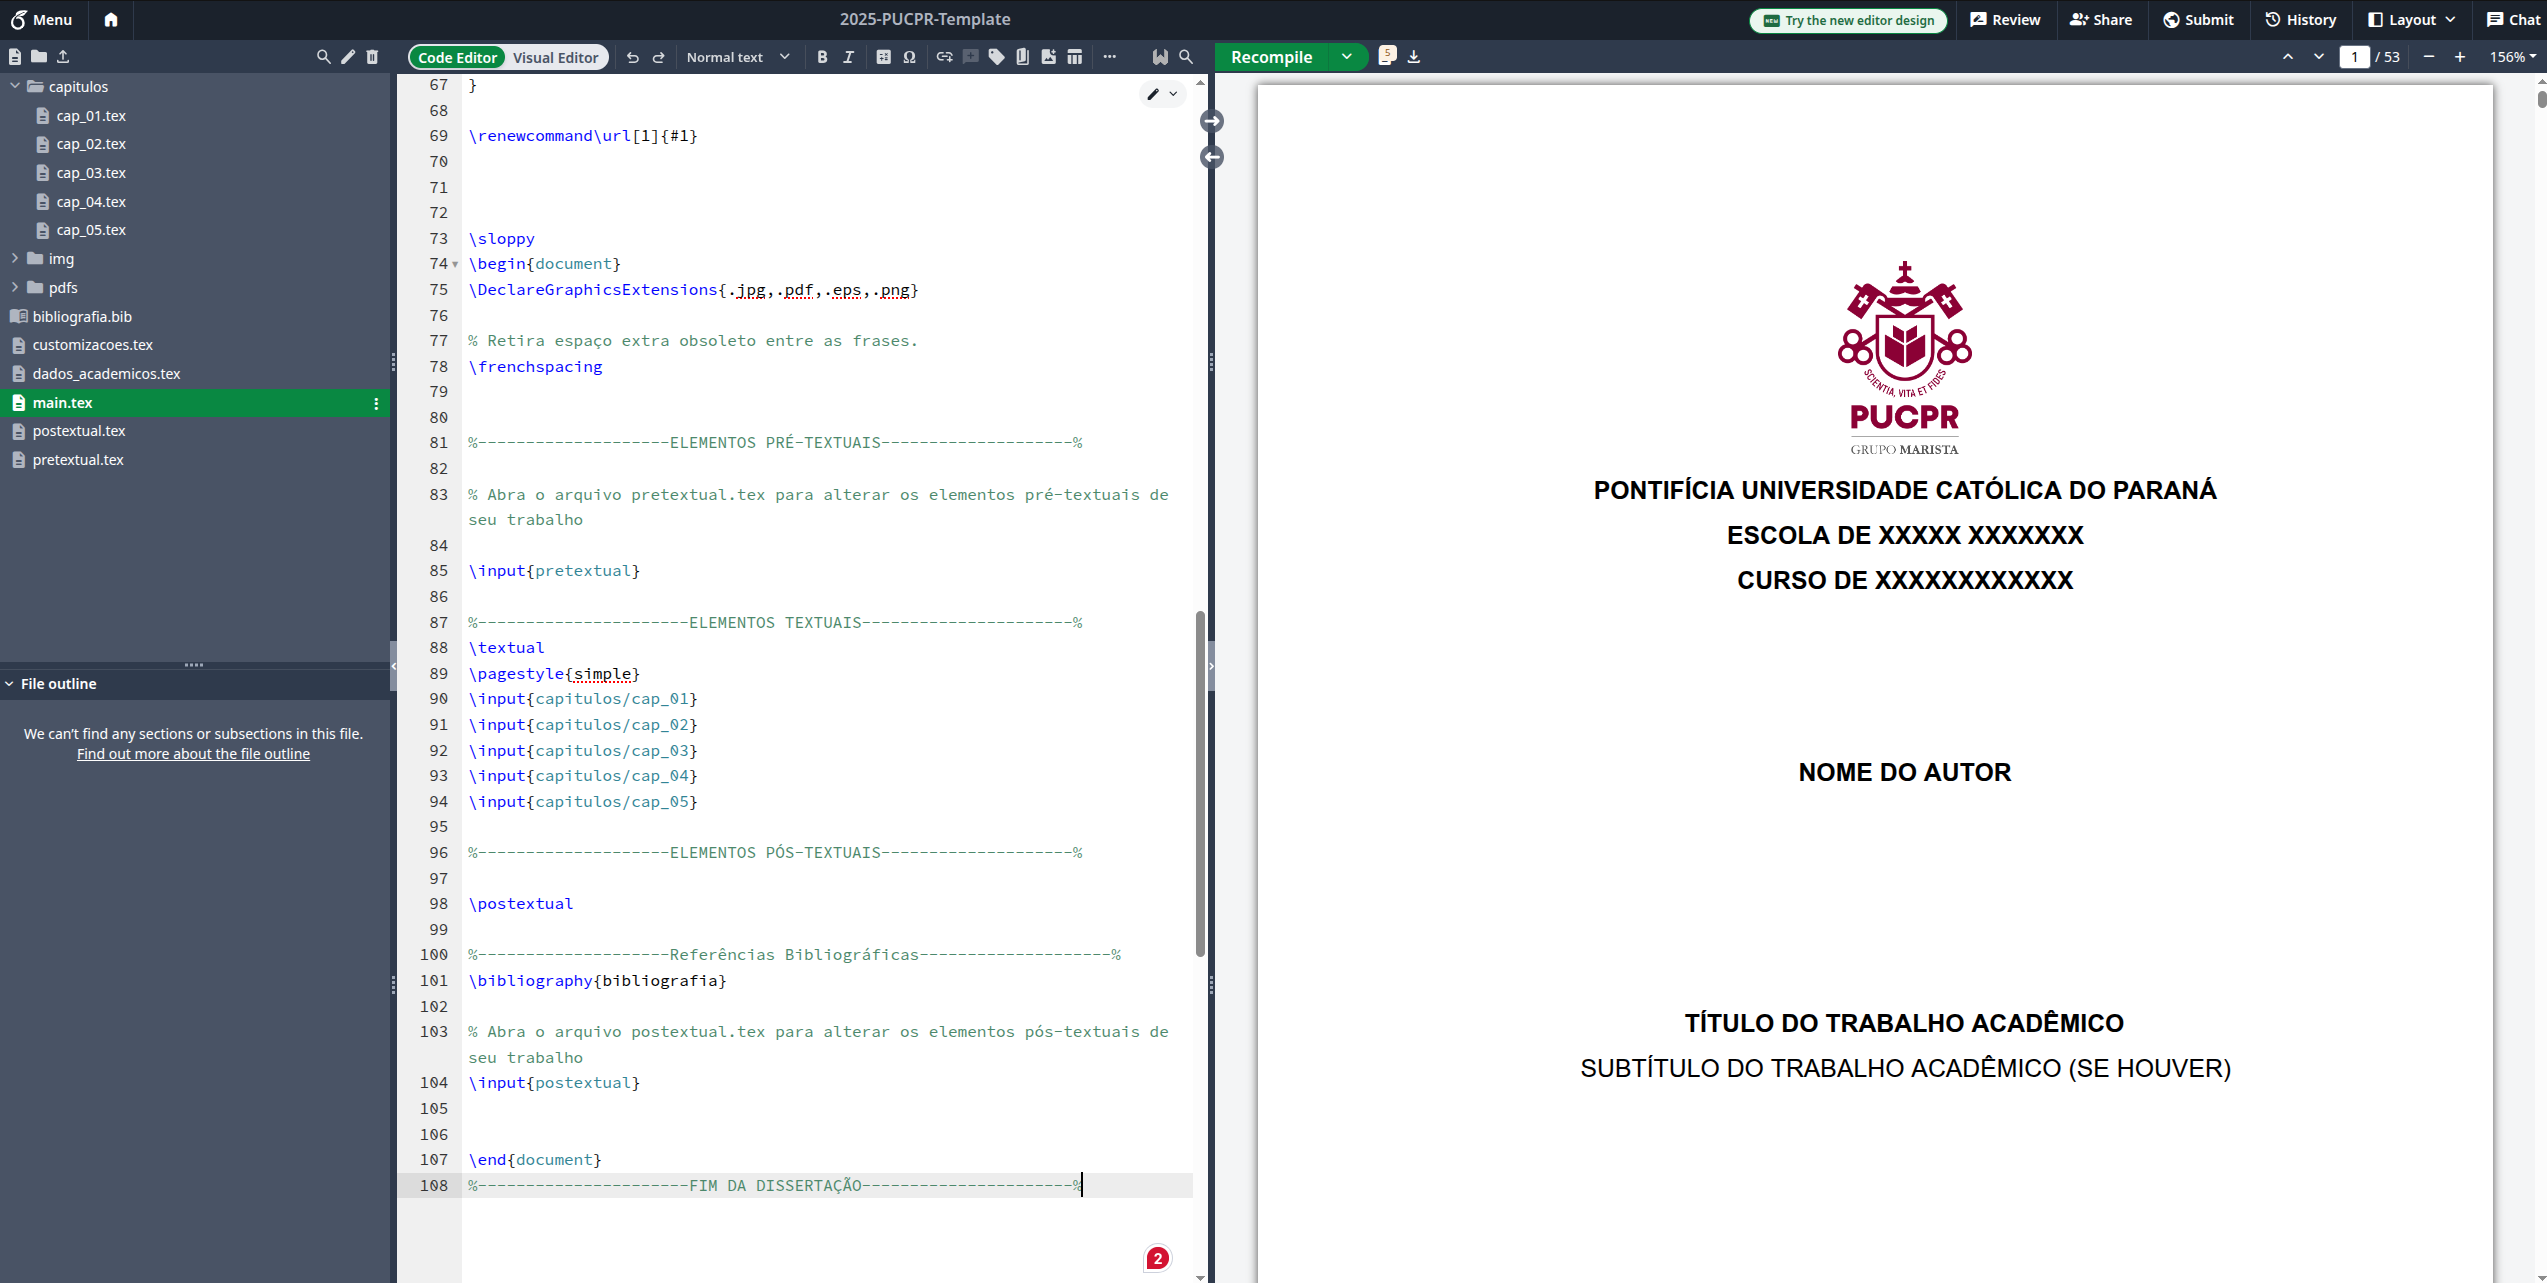
\includegraphics[width=\textwidth]{img/modelo/estrutura_arquivos.png}
    \label{fig:estrutura}
    \sourceFig{o autor, 2025.}
\end{figura}


A imagem mostra uma interface de um editor de LaTeX online  Overleaf. O editor está dividido em três seções:  Na coluna da esquerda encontra-se a estrutura de arquivos de um projeto de dissertação, com destaque para o arquivo principal: \verb|main.tex|. A coluna central mostra o documento atualmente aberto (nesse caso, o código-fonte do arquivo \verb|main.tex|). Por fim, a coluna direita apresenta uma visualização prévia do arquivo PDF produzido. 

A estrutura de arquivos da coluna esquerda é resumida a seguir:
    \begin{itemize}
        \item \verb|capitulos/|: Pasta contendo os arquivos dos capítulos do documento (\verb|cap_01.tex|, \verb|cap_02.tex|, etc.).
        \item \verb|img/|: Pasta para armazenar imagens, embora esteja colapsada e não possamos ver o conteúdo.
        \item \verb|pdfs/|: Pasta contendo vários PDFs, como anexos e apêndices (\verb|anexo_exemplo.pdf|, \verb|anexo_latex_symbols.pdf|, etc.).
        \item \verb|bibliografia.bib|: Arquivo BibTeX contendo referências bibliográficas.
        \item \verb|customizacoes.tex|: Arquivo contendo customizações específicas para o projeto.
        \item \verb|dados_academicos.tex|: Arquivo contendo informações acadêmicas (autor, título, orientador, etc.).
        \item \verb|main.tex|: Arquivo principal do documento LaTeX. É aconselhado que esteja com esse arquivo aberto sempre que necessitar \textbf{recompilar} seu projeto.
        \item \verb|postextual.tex| e \verb|pretextual.tex|: Arquivos para as partes pré-textuais e pós-textuais do documento.
    \end{itemize}

Nas seções seguintes, apresentamos uma sugestão de sequência de preenchimento do modelo para o desenvolvimento do seu documento.

\section*{2. Dados Acadêmicos}

Abra o arquivo \verb|dados_academicos.tex| e preencha as os campos referentes ao título do trabalho, subtítulo (caso não haja subtítulo, basta apagar (comentar) a linha correspondente a esse campo), autor, orientador, instituição, câmpus e data. A Figura \ref{fig:dados-academicos} ilustra um exemplo de preenchimento com dados~fictícios.

\begin{figura}{0.9\textwidth}
    \caption{Preenchimento dos dados acadêmicos.}
    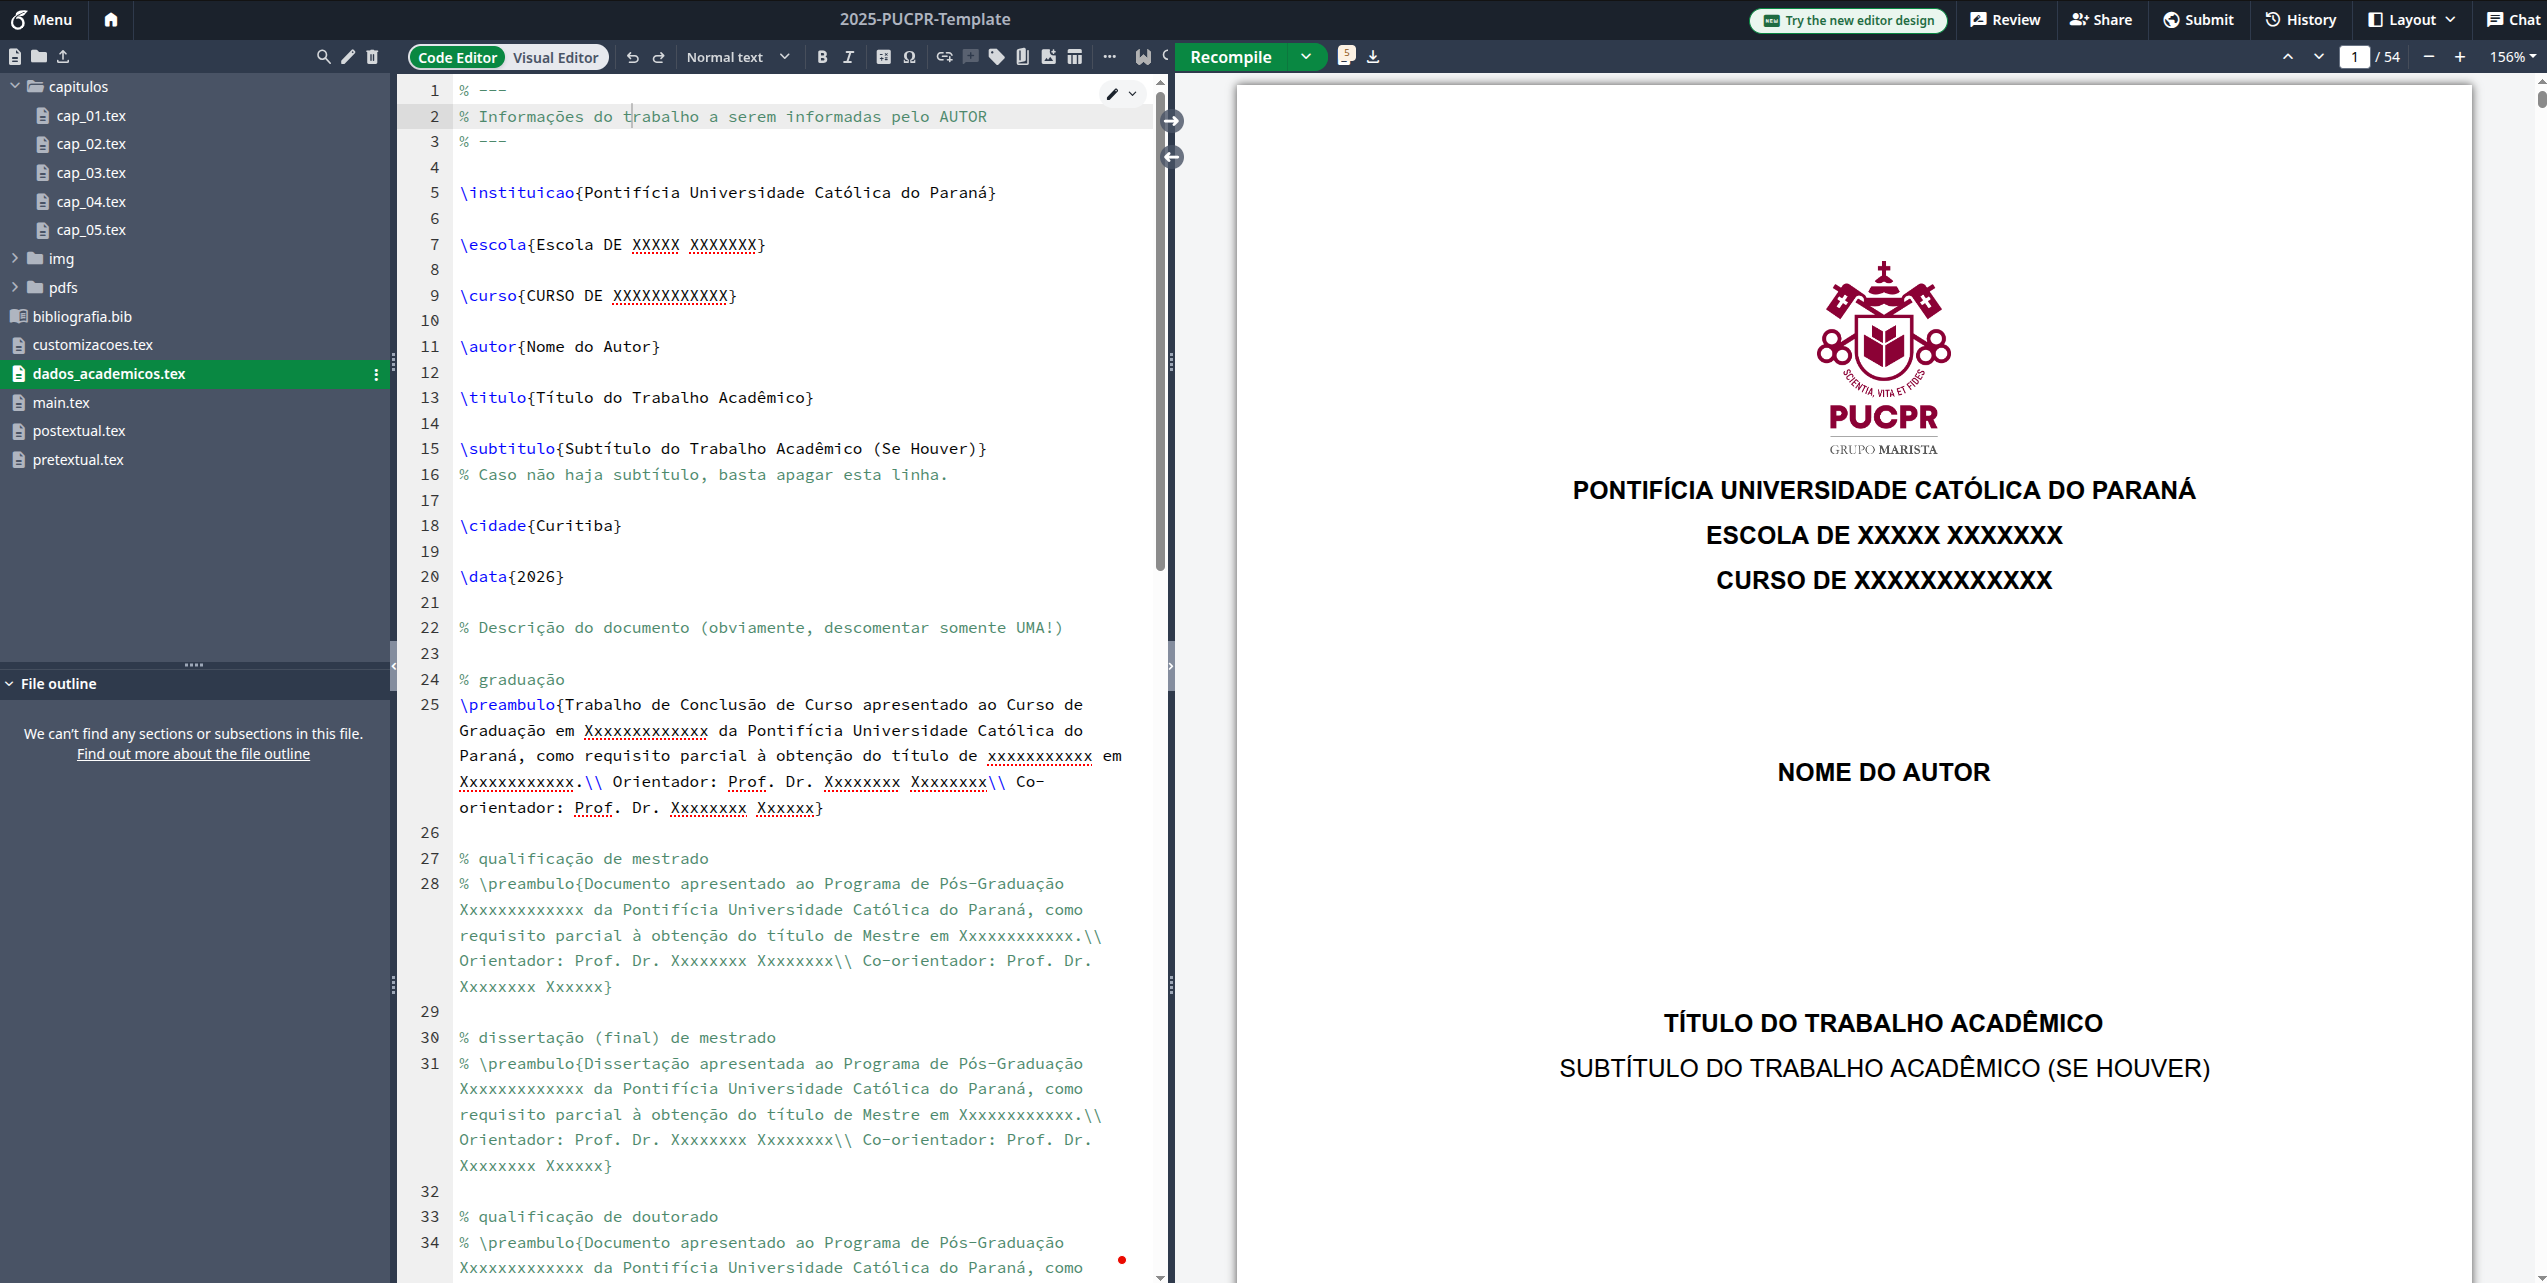
\includegraphics[width=\textwidth]{img/modelo/dados_academicos.png}
    \label{fig:dados-academicos}
    \sourceFig{o autor, 2025.}
\end{figura}

Ao clicar no botão \textbf{recompilar} do editor, os dados informados serão automaticamente carregados nos campos correspondentes tanto da capa quanto na folha de rosto do trabalho.

\section*{3. Elementos pré-textuais}

Os elementos pré-textuais são as partes iniciais de um trabalho acadêmico que antecedem o conteúdo principal. Eles são fundamentais para a estrutura e apresentação do documento, fornecendo informações essenciais sobre o trabalho, seus autores e orientadores, bem como a instituição\footnote{Para mais detalhes sobre os elementos pré-textuais (obrigatórios e opcionais), leia a norma ABNT NBR 14724 \cite{nbr14724}}.

Abra o arquivo \verb|pretextual.tex|. A seguir, mostra-se o preenchimento das principais informações pré-textuais.

A Figura \ref{fig:pretextual-01} mostra os primeiros quatro elementos pré-textuais: Capa, Folha de Rosto, Ficha Catalográfica e Folha de Aprovação. Quanto aos dois primeiros, nenhuma intervenção é necessário pois são elementos de formatação padronizada cujos dados foram informados no arquivo \verb|dados_academicos.tex| como detalhado na seção anterior.

\begin{figura}{0.9\textwidth}
    \caption{Elementos pré-textuais: Ficha catalográfica e Folha de aprovação.}
    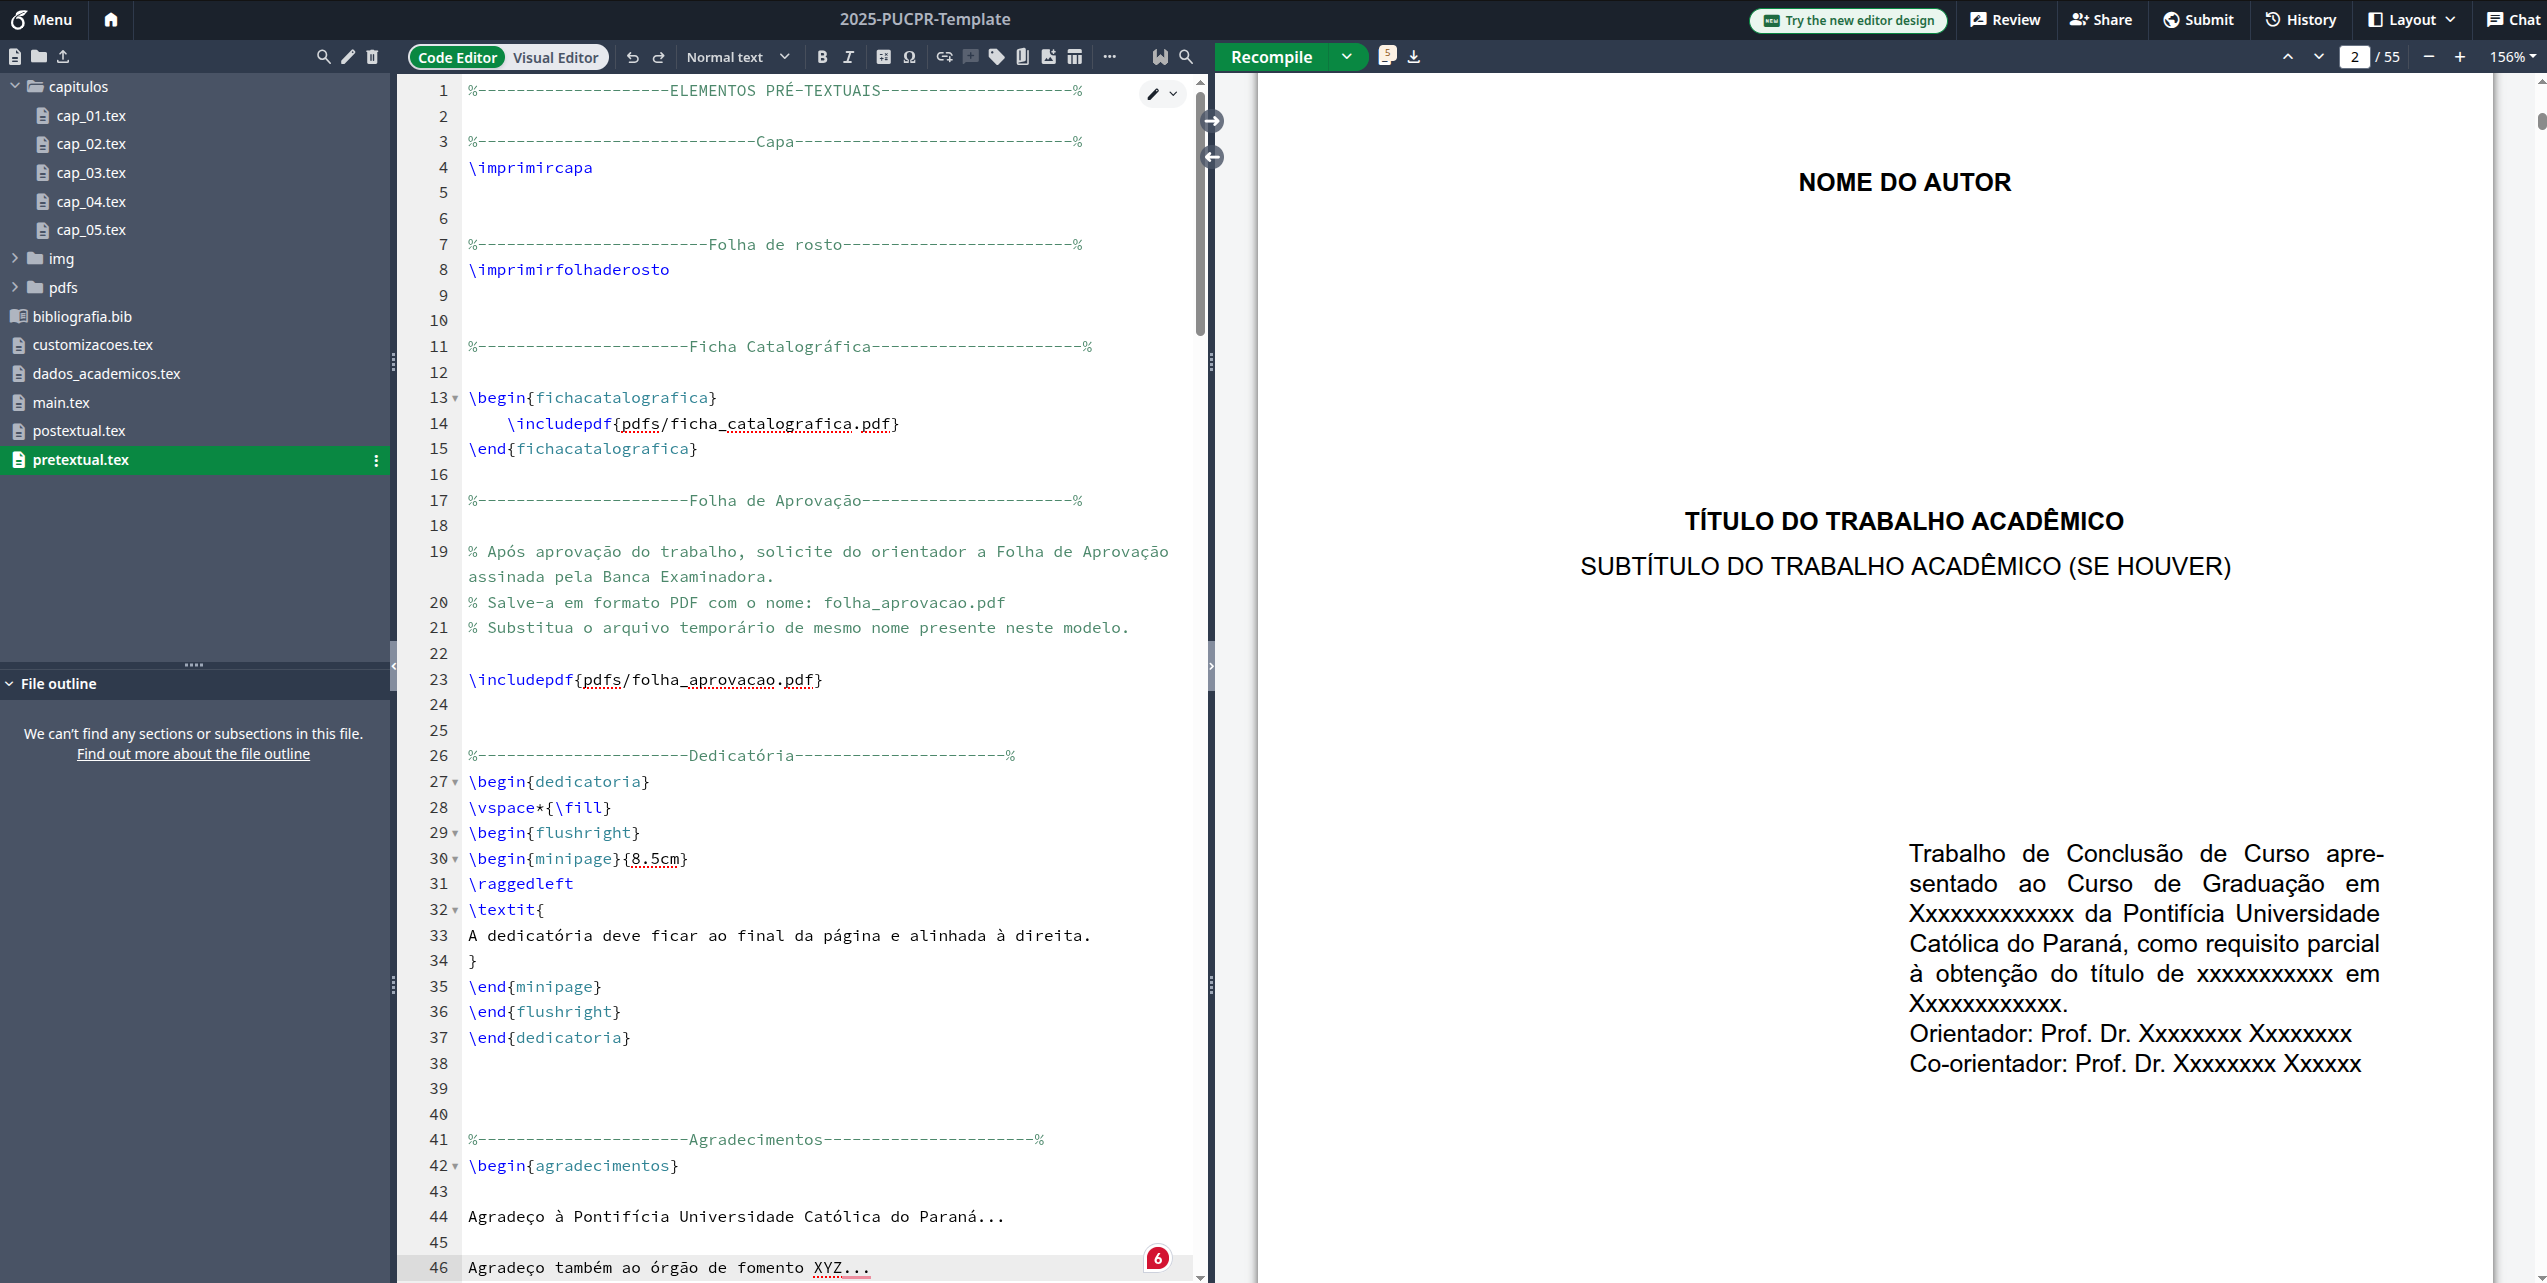
\includegraphics[width=\textwidth]{img/modelo/pretextual-01.png}
    \label{fig:pretextual-01}
    \sourceFig{o autor, 2025.}
\end{figura}

A respeito da Ficha Catalográfica e da Folha de Aprovação, tratam-se de documentos cujo preenchimento ocorrerá após a aprovação do trabalho e as correções sugeridas pela Banca Examinadora.

\subsection*{3.1 Ficha Catalográfica}
Após a aprovação do trabalho, faça o download da ficha em formato PDF e salve-a com o nome: \verb|ficha_catalografica.pdf| dentro da pasta \verb|pdfs|. 

\subsection*{3.2 Folha de Aprovação}

Após aprovação do trabalho, solicite ao orientador a Folha de Aprovação assinada pela Banca Examinadora. Salve-a em formato PDF com o nome: \verb|folha_aprovacao.pdf|. Substitua o arquivo temporário de mesmo nome presente na pasta \verb|pdfs| neste modelo.


Nos dois casos acima, esteja atento para o correto nome de arquivos, bem como o local em que devem ser salvos. Ao clicar em \textbf{Recompilar}, os novos arquivos serão carregados em seu trabalho.

Os próximos elementos pré-textuais são: Dedicatória, Agradecimentos e Epígrafe. Seu preenchimento é bastante intuitivo, conforme mostrado na Figura \ref{fig:pretextual-02}.

\begin{figura}{0.9\textwidth}
    \caption{Elementos pré-textuais: Dedicatória, Agradecimentos e Epígrafe.}
    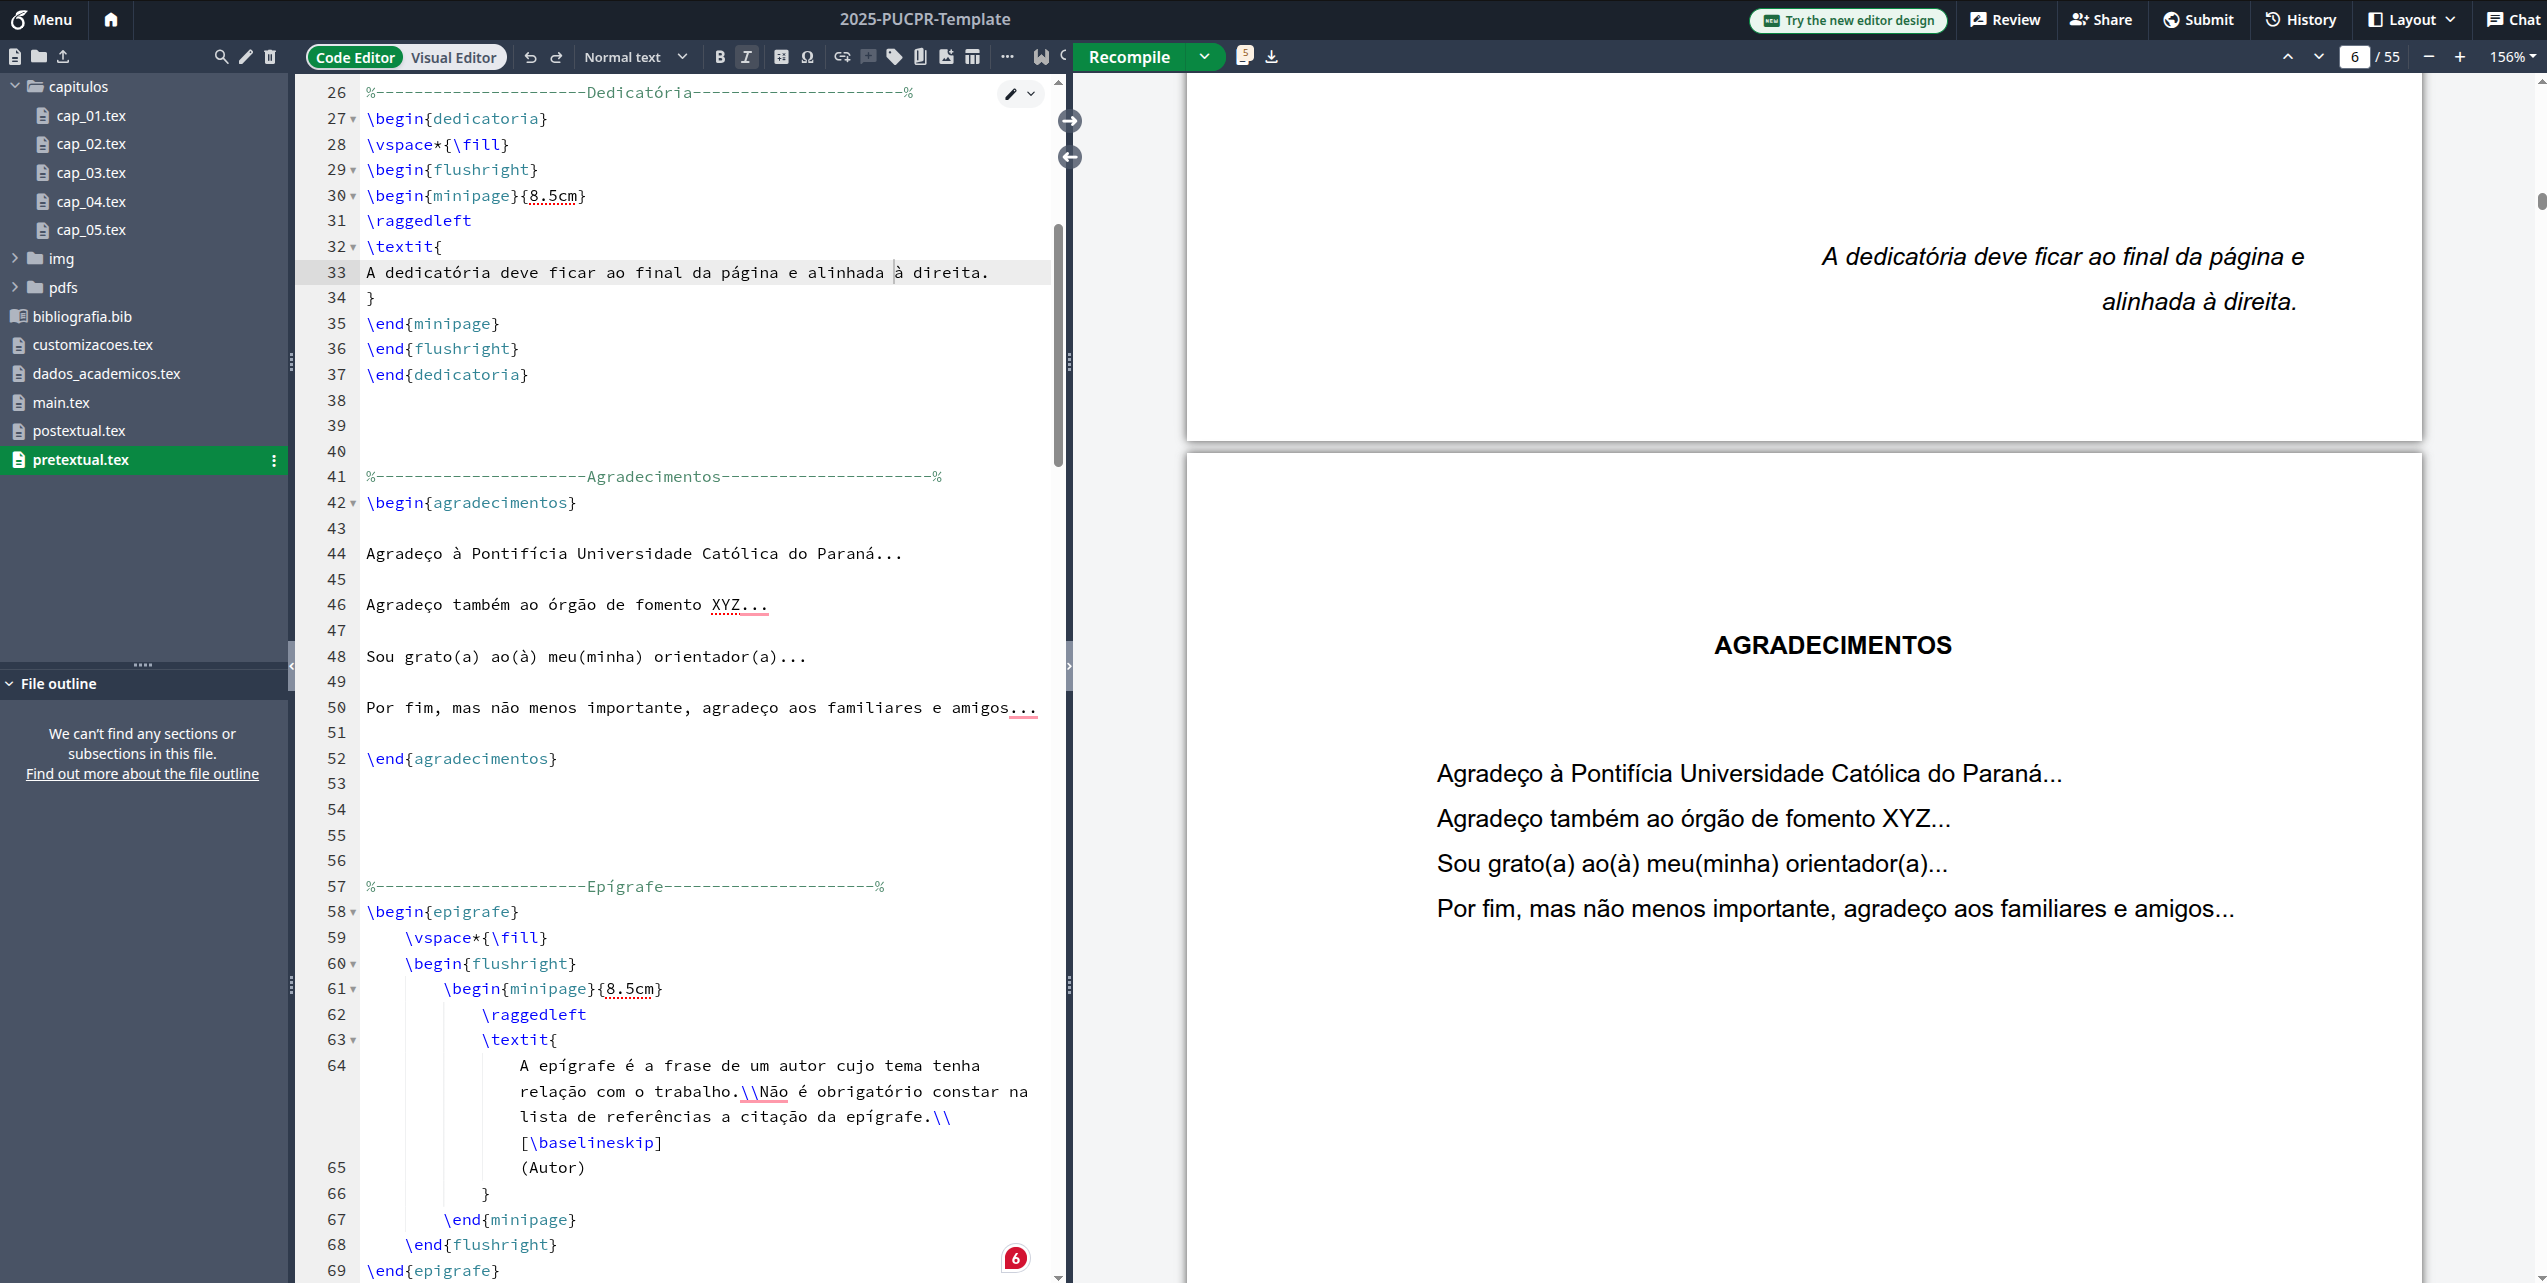
\includegraphics[width=\textwidth]{img/modelo/pretextual-02.png}
    \label{fig:pretextual-02}
    \sourceFig{o autor, 2025.}
\end{figura}


Em seguida, tem-se o resumo (em língua portuguesa e em língua estrangeira), conforme mostrado na Figura \ref{fig:pretextual-03}. Observe que de acordo com a norma ABNT NBR 6028:2021 o resumo deve apresentar o conteúdo do trabalho de  forma sucinta, composto por uma sequência de frases concisas em parágrafo único, sem enumeração de tópicos e escritas com verbo na terceira pessoa \cite{nbr6028}.

\begin{figura}{0.9\textwidth}
    \caption{Elementos pré-textuais: Resumo e Abstract.}
    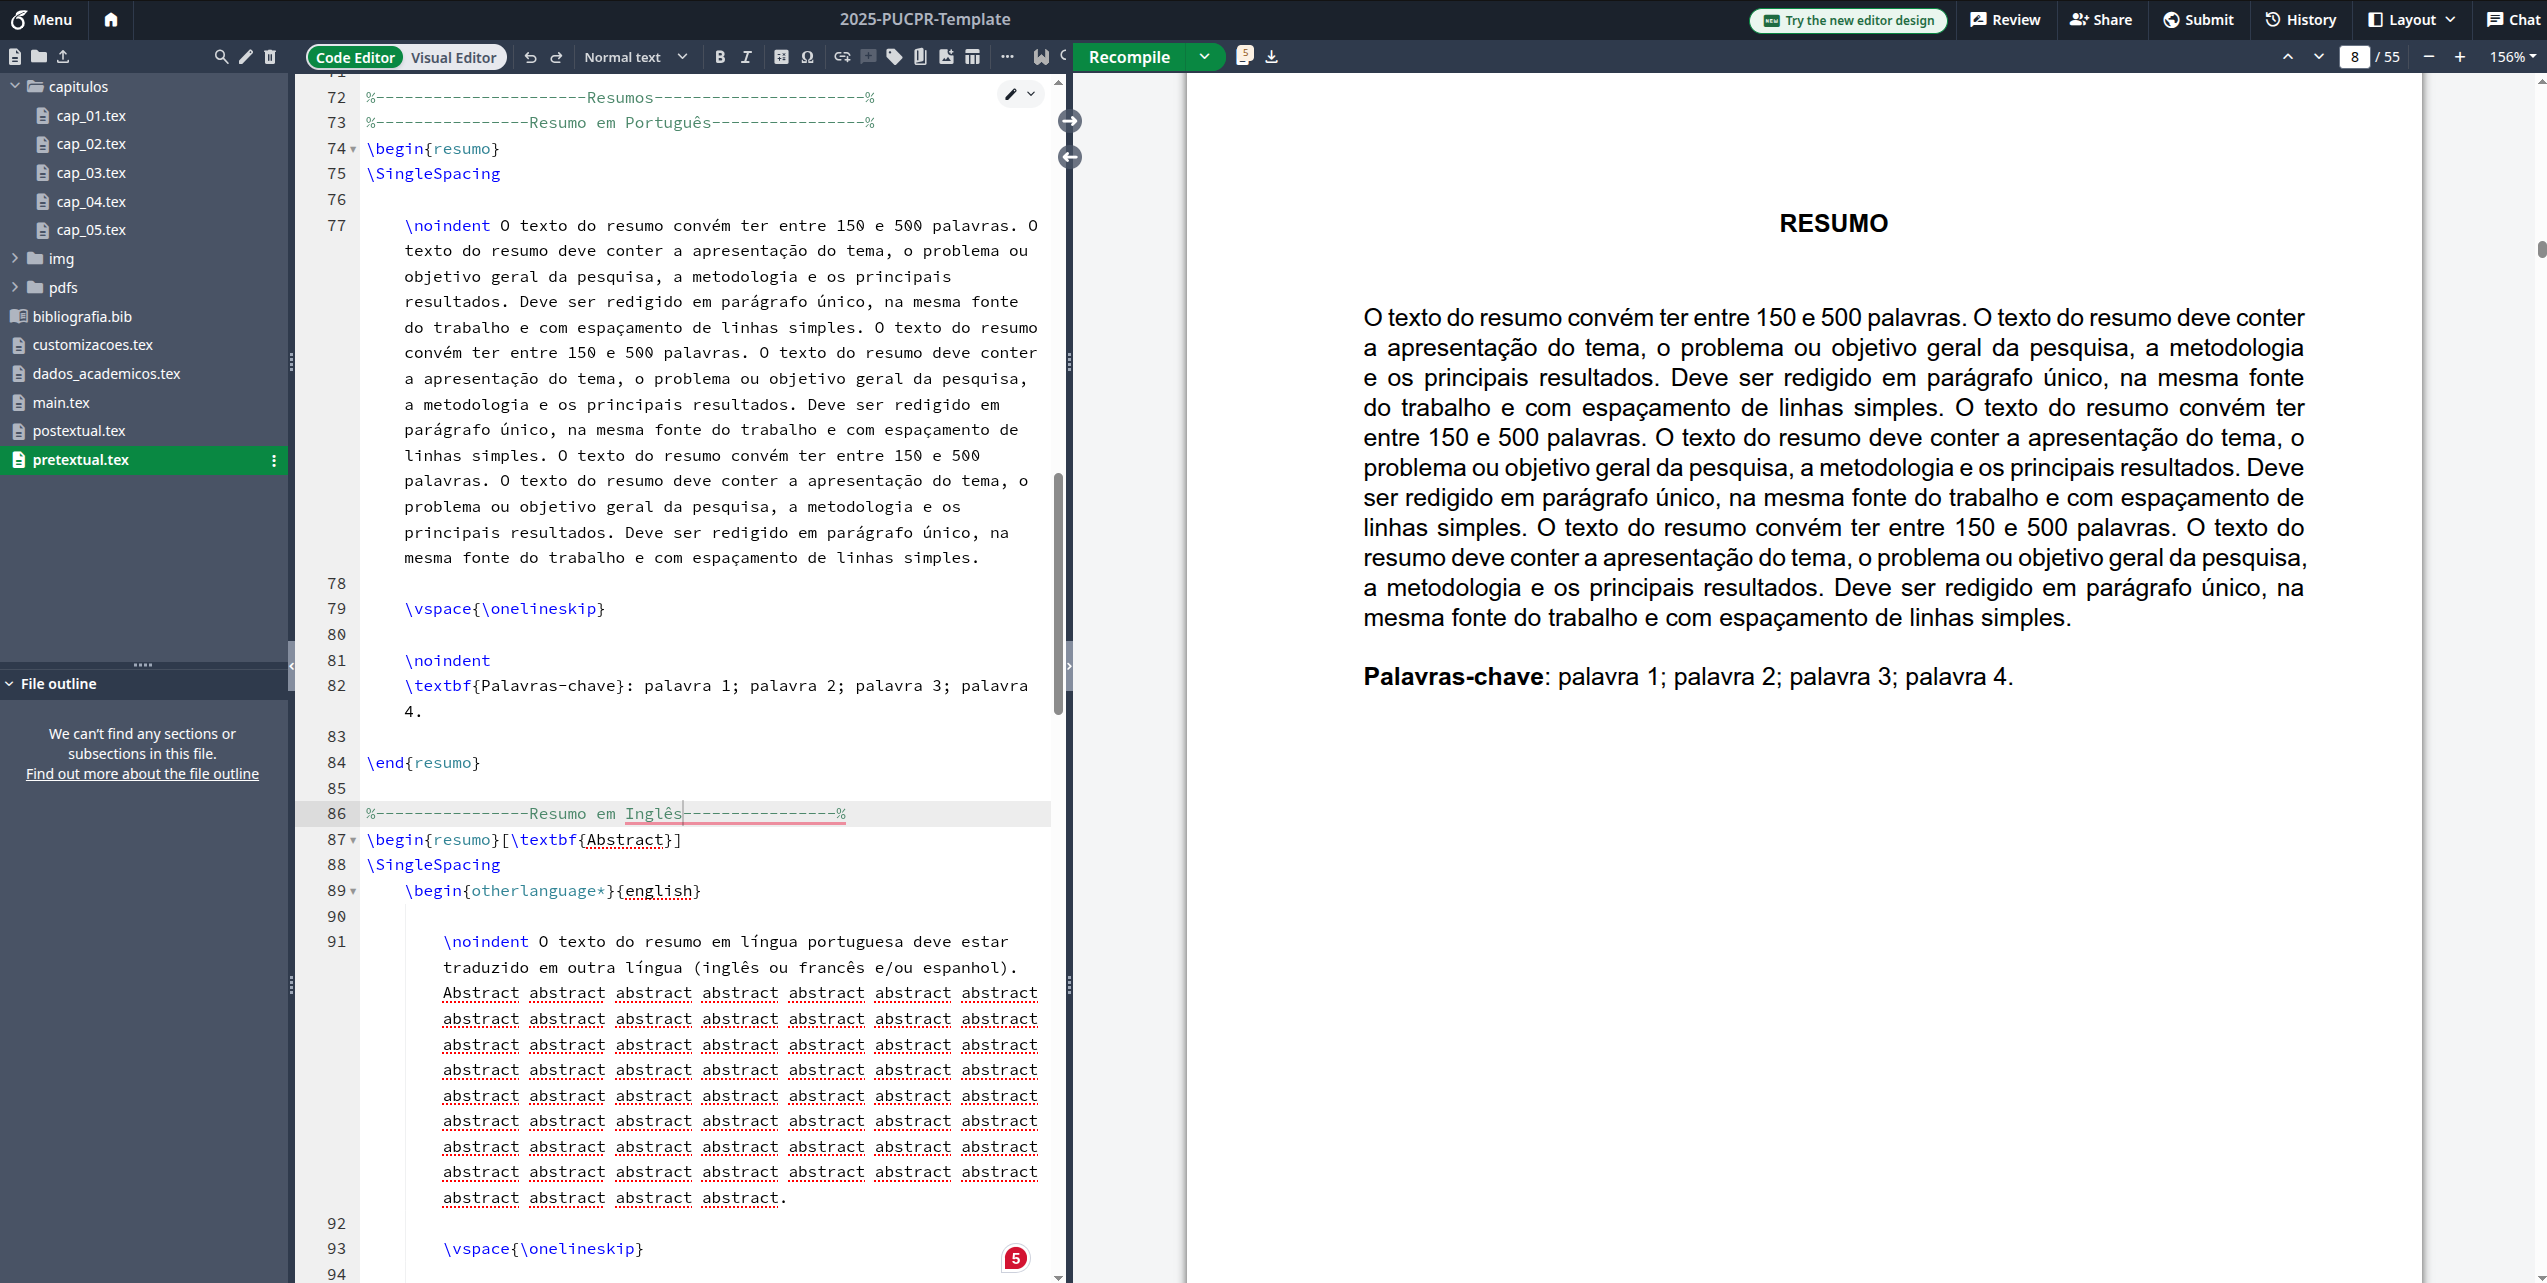
\includegraphics[width=\textwidth]{img/modelo/pretextual-03.png}
    \label{fig:pretextual-03}
    \sourceFig{o autor, 2025.}
\end{figura}

Quanto às palavras-chave, segundo a norma ABNT NBR 6028:2021, devem ser separadas entre si por ponto e vírgula e finalizadas por ponto.  A referida norma ainda ressalta que as palavras-chave devem ser grafadas com iniciais em letras minúsculas, exceto quando substantivos próprios e nomes científicos \cite{nbr6028}.

Uma importante parte  dos elementos pré-textuais são as listas. A Figura \ref{fig:pretextual-04} mostra as listas de ilustrações, quadros, tabelas, abreviaturas e siglas e símbolos.


\begin{figura}{0.9\textwidth}
    \caption{Elementos pré-textuais: Listas.}
    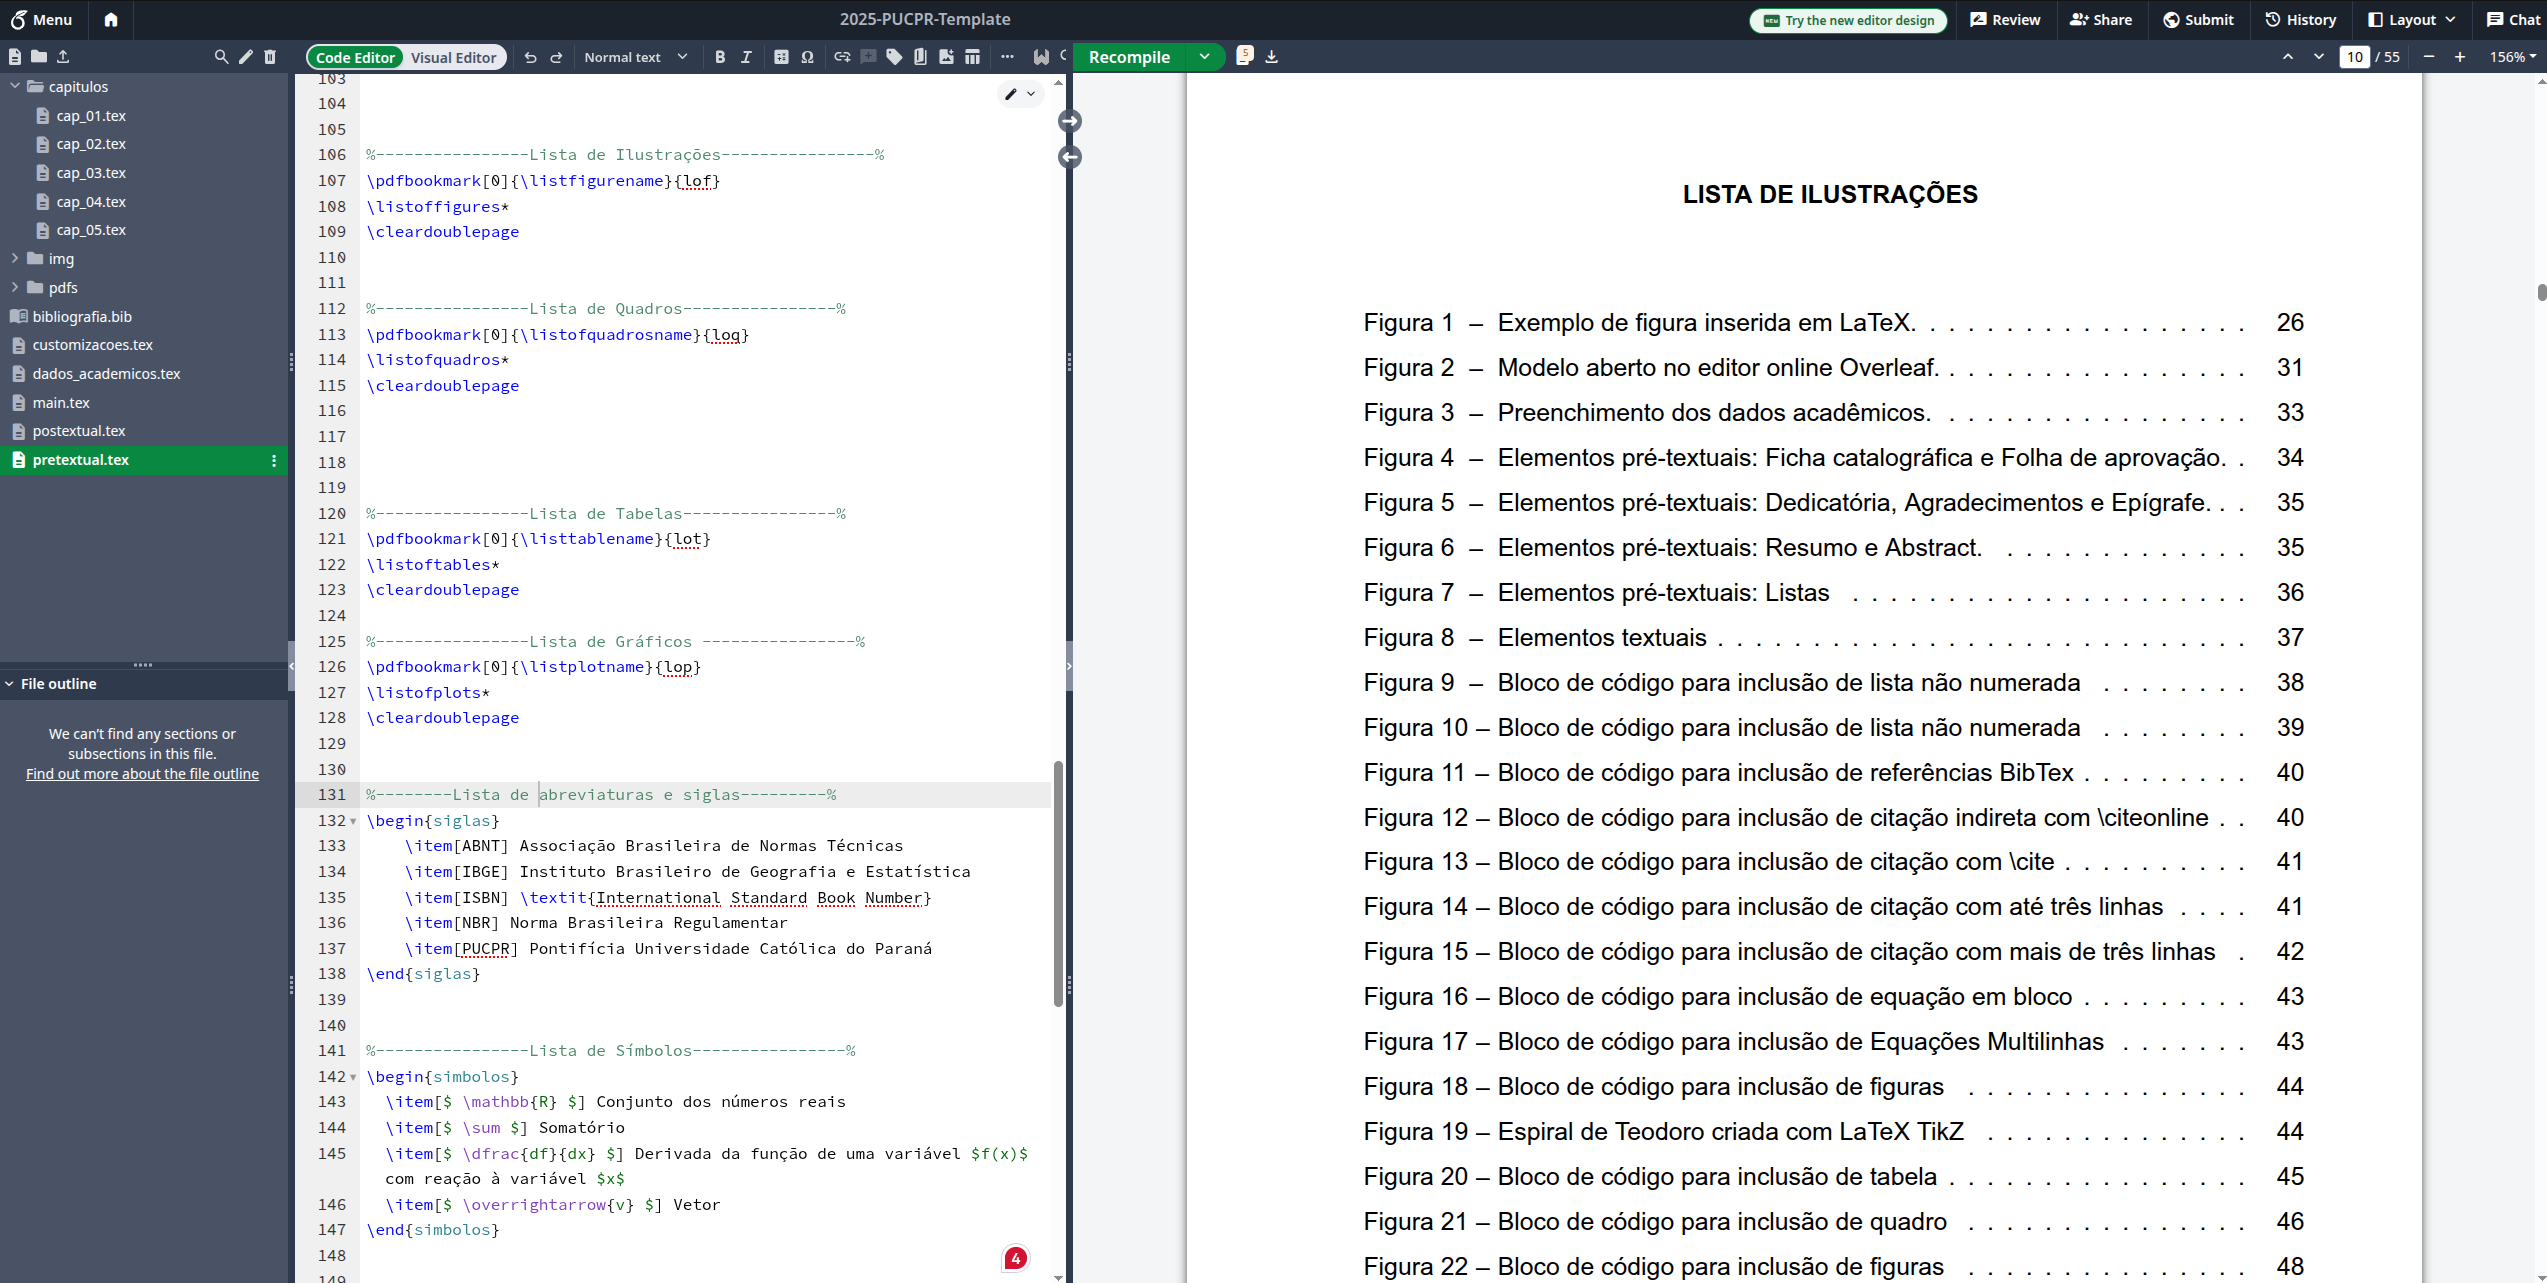
\includegraphics[width=\textwidth]{img/modelo/pretextual-04.png}
    \label{fig:pretextual-04}
    \sourceFig{o autor, 2025.}
\end{figura}

Observe que a Listas de Ilustrações, a Lista de Quadros e a Lista de Tabelas são criadas automaticamente, à medida que estes elementos são incluídos no texto do trabalho. Portanto, apenas a Lista de Abreviaturas e Siglas  e a Lista de Símbolos requerem preenchimento manual pelo autor do trabalho. Alguns exemplos podem ser encontrados no arquivo \verb|pretextual.tex|.

Para finalizar a parte de elementos pré-textuais, tem-se o sumário. À  medida que o autor adiciona novos capítulos (\verb|\chapter{|), seções (\verb|\section|) e subseções (\verb|\subsection|), o sumário será atualizado automaticamente.

\section*{4. Elementos Textuais}

Para uma melhor organização do trabalho, a parte textual do documento foi dividida em capítulos: \verb|cap_01.tex|, \verb|cap_02.tex|, \verb|cap_03.tex|, \verb|cap_04.tex| e \verb|cap_05.tex| dentro na pasta \verb|capitulos|.  Note que o carregamento desses arquivos para a dissertação é feito por meio do comando \verb|\input| no arquivo principal \verb|main.tex|, como mostrado na Figura \ref{fig:textual-01}.

\begin{figura}{0.9\textwidth}
    \caption{Elementos textuais.}
    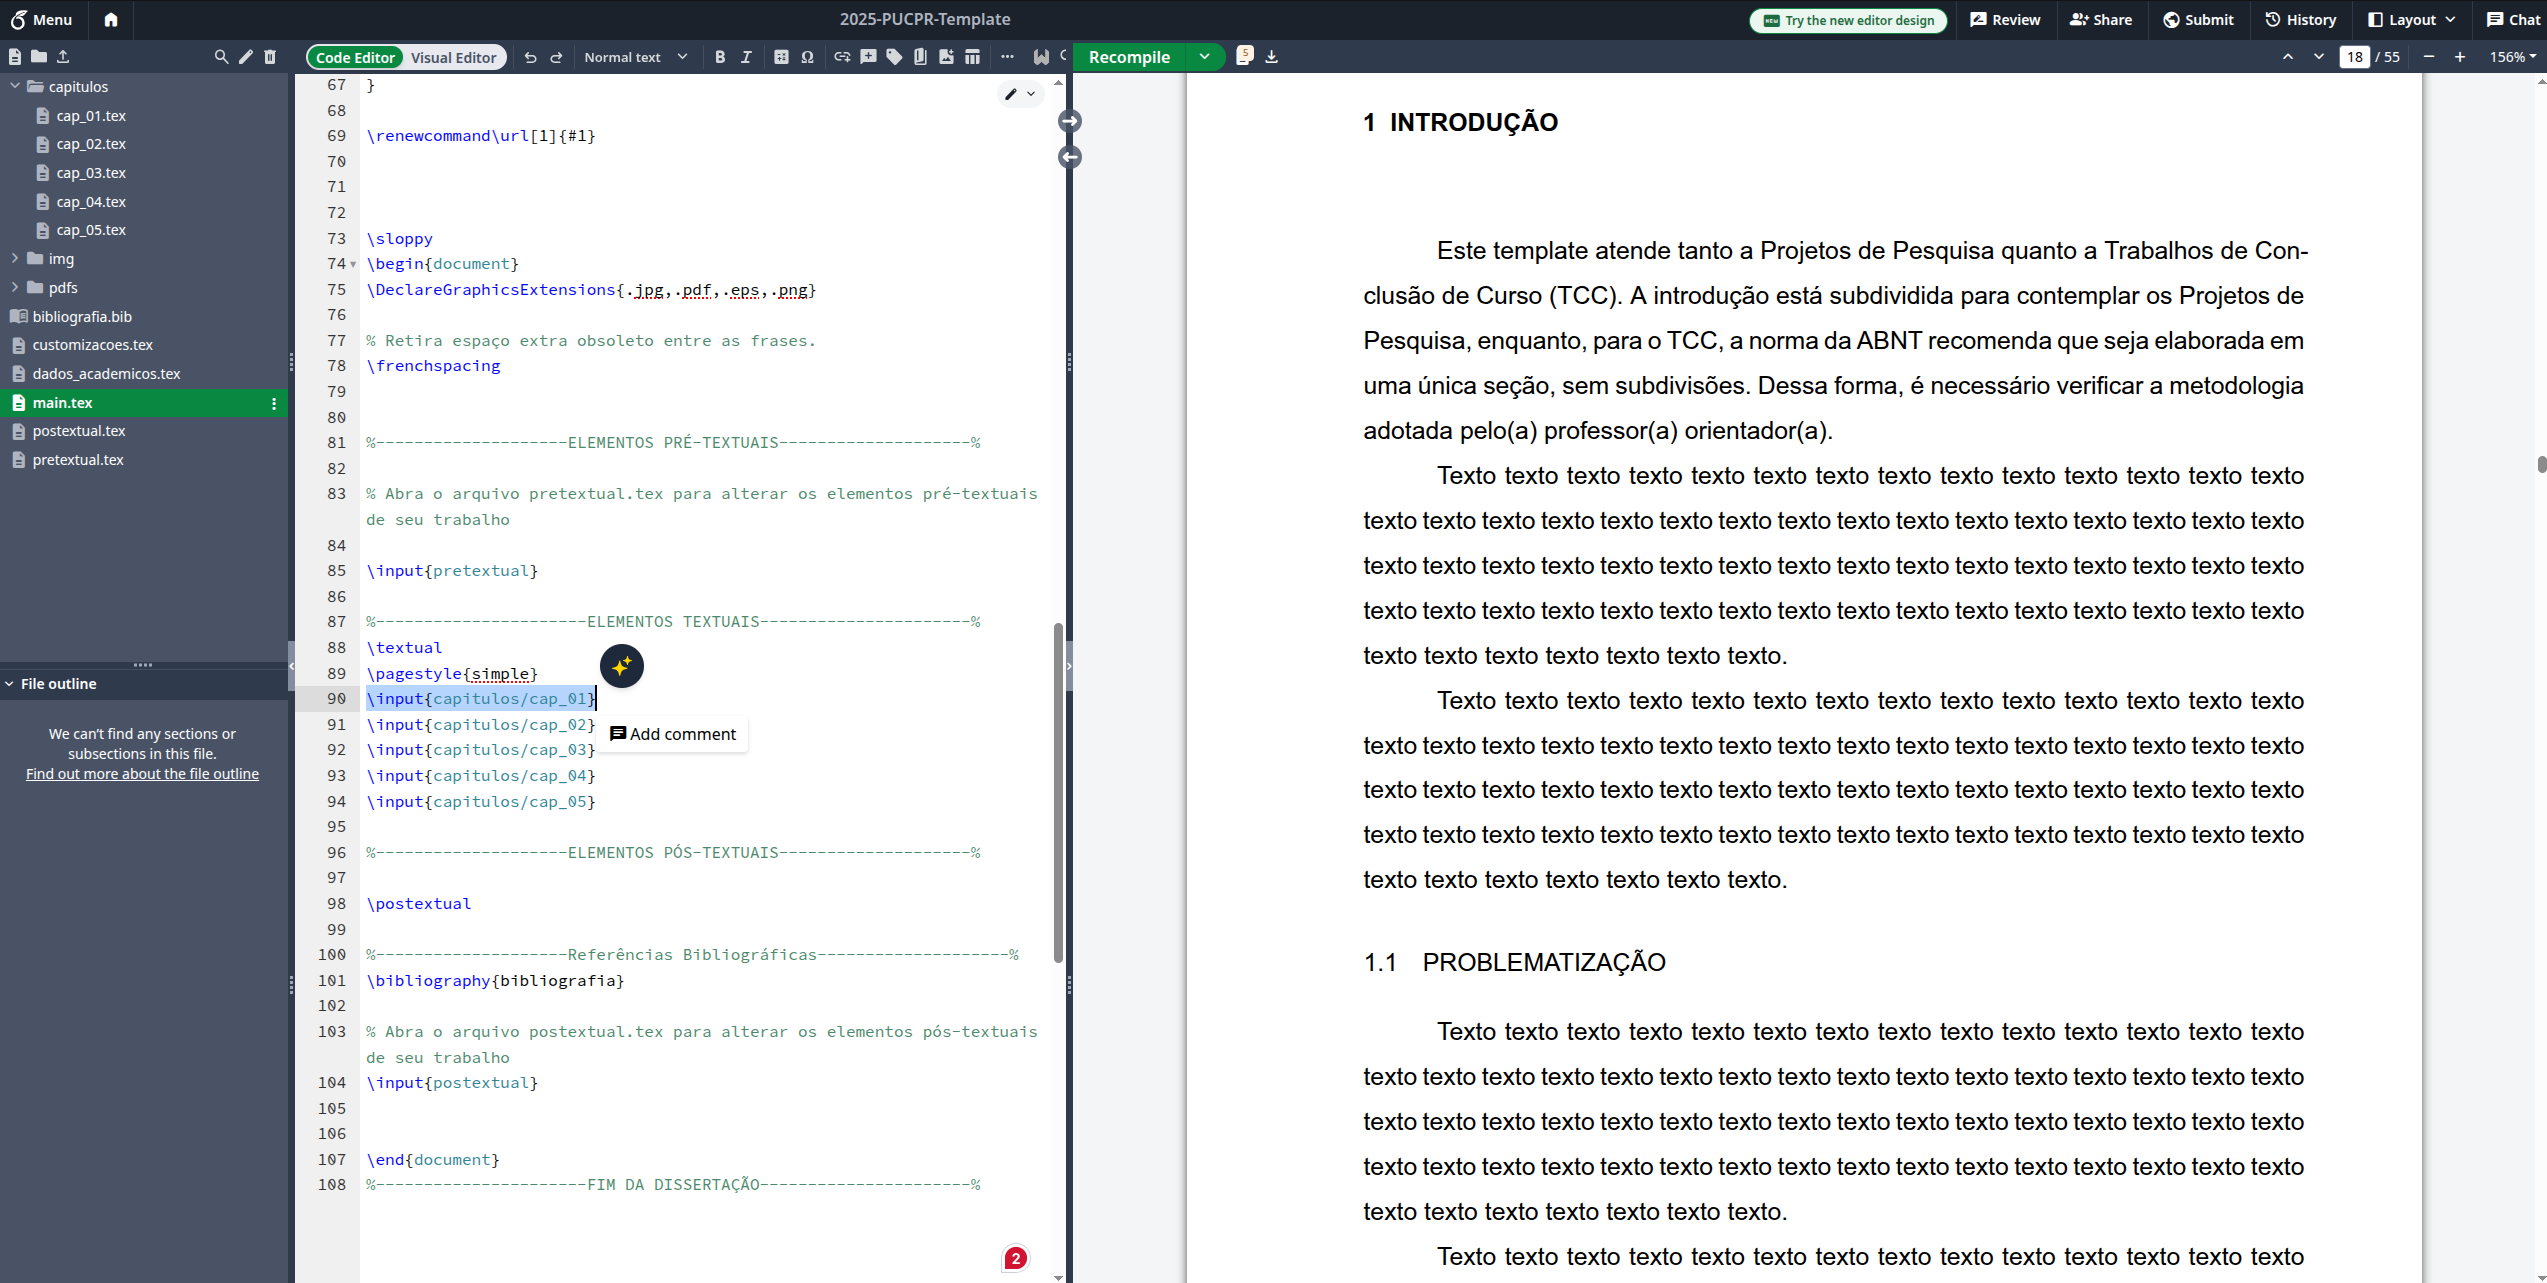
\includegraphics[width=\textwidth]{img/modelo/textual-01.png}
    \label{fig:textual-01}
    \sourceFig{o autor, 2025.}
\end{figura}

Observe na Figura \ref{fig:textual-01} que para a inclusão do arquivo \verb|cap_01.tex| foi utilizado o comando \verb|%----------------Cap_01----------------%
\chapter{Introdução}

% ------------------------------------------------------------
% Contextualização
% ------------------------------------------------------------
O crescimento acelerado dos veículos aéreos não tripulados (VANTs) nas últimas décadas transformou setores como logística, monitoramento ambiental, agricultura de precisão e defesa. Plataformas de decolagem e aterrissagem vertical (VTOL), em particular os quadrotores, tornaram-se objetos de intensa investigação em razão de suas capacidades únicas de manobra, todavia impõem desafios igualmente expressivos de controle: dinâmica intrínsecamente não-linear, acoplamento entre eixos e forte sensibilidade a perturbações externas como rajadas de vento \cite{nguyen2020}. A operação segura e eficiente dessas plataformas exige algoritmos capazes de satisfazer simultaneamente requisitos de precisão de rastreamento, rejeição robusta a perturbações e execução em tempo real sob severas restrições computacionais dos microcontroladores embarcados.

Nesse contexto, o aeropêndulo consolida-se como uma bancada de experimentação, onde sistema reproduz a dinâmica essencial de um rotor VTOL em um único grau de liberdade, permitindo a comparação controlada de estratégias de controle em laboratório. Sua dinâmica não-linear, determinada pelo torque aerodinâmico do conjunto motor-hélice e pela não-linearidade gravitacional intrínseca ao pêndulo, exige técnicas de controle além dos métodos lineares clássicos. A bancada utilizada neste trabalho foi originalmente projetada e construída por \citeonline{lima2025}, cujo sistema mecânico e eletrônico é reaproveitado e estendido com novos algoritmos de controle.

% ------------------------------------------------------------
% Motivação / Justificativa
% ------------------------------------------------------------
O Controle Preditivo Não-Linear (NMPC) destaca-se entre as estratégias avançadas por combinar tratamento explícito de restrições, previsão do comportamento futuro da planta e desempenho reconhecidamente superior ao PID clássico em sistemas não-lineares \cite{mayne2000}. No entanto, a solução repetida de um Problema de Controle Ótimo a cada período de amostragem implica um custo computacional que pode ultrapassar os recursos disponíveis em microcontroladores de baixo custo operando em dinâmicas rápidas. Plataformas VTOL de pequeno porte tipicamente exigem períodos de amostragem da ordem de 10\,ms, intervalo que representa uma barreira prática para a implantação direta do NMPC em unidades de baixo poder computacional.

A abordagem de MPC aproximado por redes neurais surge como alternativa promissora, uma rede treinada offline para imitar a política do NMPC pode ser avaliada em tempo de inferência constante e reduzido, compatível com microcontroladores de classe Cortex-M \cite{karg2020}. A substituição da otimização repetida por uma única passagem \textit{feedforward} reduz o custo computacional em ordens de grandeza sem exigir reformulação do modelo ou dos objetivos de controle, tornando a estratégia particularmente atrativa para implantação embarcada em sistemas com restrições rígidas de memória e tempo \cite{david2021}.

% ------------------------------------------------------------
% Revisão da Literatura
% ------------------------------------------------------------
\section{Estado da Arte}

\subsection{Controle clássico}
Controladores clássicos como o PID (Proporcional-Integral-Derivativo) são a espinha dorsal de inúmeras aplicações industriais e robóticas. O desenvolvimento formal dessa lei de controle, também conhecida como controle de três termos, foi apresentado em 1922 pelo engenheiro Nicolas Minorsky \cite{bennett1996}.

Em plataformas ágeis, como VANTs, o controle PID muitas vezes não é suficiente de forma isolada, sendo relegado a uma malha interna de controle de atitude ou velocidade, o que cria a necessidade de controladores externos mais sofisticados capazes de garantir estabilidade sistêmica otimizada. Esse cenário motiva a adoção de algoritmos mais avançados, como o Controle Preditivo Baseado em Modelo (MPC), capaz de gerenciar diretamente sistemas de múltiplas entradas e múltiplas saídas com restrições operacionais rígidas \cite{nguyen2020}.

\subsection{Controle Preditivo Não-Linear}
O Controle Preditivo Não-Linear (NMPC) fundamenta-se na resolução de um problema de controle ótimo em tempo discreto e horizonte finito, em que um otimizador avalia um modelo preditivo para minimizar uma função de custo ao longo do horizonte de predição, lidando ativamente com restrições de estado e entrada. Uma de suas maiores vantagens em relação ao PID clássico é a característica de \textit{preview} (visão antecipada), pela qual o controlador avalia o comportamento futuro e reage a referências antes mesmo do erro se acumular \cite{mayne2000}. Embora o elevado custo computacional de resolver iterativamente online o problema de Programação Não-Linear (NLP) seja um desafio para o hardware embarcado, a adoção de métodos de otimização diretos reduz drasticamente a carga de processamento, viabilizando a aplicação do NMPC mesmo na dinâmica inerentemente rápida de robôs aéreos \cite{nguyen2020}.

\subsection{MPC Explícito e suas limitações}
Buscando contornar o custo computacional da otimização online, surgiu o conceito de MPC Explícito (EMPC). Nessa abordagem, a lei de controle é pré-computada offline por meio da resolução de um problema de programação multiparamétrica, resultando em uma função afim por partes (PWA) definida sobre partições politópicas do espaço de estados, a execução online resume-se, então, a identificar o polítopo atual e aplicar a equação correspondente \cite{bemporad2002}. A principal limitação de escalabilidade do EMPC reside no crescimento exponencial do número de regiões politópicas à medida que o horizonte de predição e o número de restrições aumentam, tornando sua aplicação em sistemas embarcados restrita a problemas de baixíssima dimensionalidade \cite{bemporad2002}. Esse gargalo motiva fortemente a adoção de abordagens de aproximação da lei de controle por inteligência artificial, como o uso de redes neurais \cite{alsmeier2024}.

\subsection{Aproximação de leis de controle por redes neurais}
A limitação de escalabilidade de memória do EMPC impulsiona a aproximação da sua lei de controle explícita por uma rede neural previamente treinada. \citeonline{karg2020} demonstraram matematicamente que Redes Neurais Profundas (DNNs) com funções de ativação ReLU conseguem representar de maneira exata as funções afins por partes das leis de controle do MPC. O principal desafio técnico desta abordagem recai sobre o erro de aproximação e a perda de garantias intrínsecas do MPC original. Para lidar com os \textit{trade-offs} entre tamanho do modelo e segurança, pesquisadores aplicam a Desigualdade de Hoeffding para conferir limites estatísticos e garantir a satisfação de restrições com alta probabilidade \cite{hertneck2018}; alternativamente, derivam-se limites no pior caso via constantes de Lipschitz para certificar que os desvios da rede em relação à lei nominal estão contidos no limite de robustez
\cite{alsmeier2024}.

\subsection{Identificação de sistemas para alimentar o NMPC}
Para a concepção offline de um projeto de NMPC, a precisão do modelo preditivo subjacente é vital para as predições de estados. Muitos sistemas, como motores BLDC em um aeropêndulo, exibem atritos e aerodinâmicas difíceis de modelar analiticamente. Nesses casos, a identificação baseada em dados de entrada e saída torna-se altamente efetiva. A partir de ensaios experimentais, é possível treinar modelos de predição que capturam os efeitos dinâmicos dominantes, incluindo não-linearidades aerodinâmicas negligenciadas pelos modelos físicos clássicos, e integrá-los diretamente ao esquema MPC \cite{jiang2022}.

\subsection{Redes neurais MLP arquitetura e treinamento supervisionado} A fim de aproximar a política de controle, as Redes Neurais \textit{Feedforward} (FFNN), ou Perceptrons Multicamadas (MLP), mostram-se candidatas ideais devido à sua capacidade de mapeamento estático livre de \textit{delays} recorrentes. A arquitetura típica consiste em camadas ocultas com funções de ativação ReLU e uma camada de saída linear. A geração do \textit{dataset} se da pela exploração em malha fechada do controlador MPC exato sobre estados iniciais diversos, registrando-se os pares de ``estado atual'' $\rightarrow$ ``ação de controle ótima''; o treinamento subsequente ocorre com aprendizado supervisionado focado em minimizar o Erro Quadrático Médio (MSE), por meio de algoritmos baseados em descida de gradiente estocástico, como o otimizador Adam \cite{karg2020}.

\subsection{Inferência de redes neurais em hardware embarcado (TinyML)} Executar algoritmos preditivos em microcontroladores (MCUs) requer superar restrições críticas de memória e frequência de relógio típicas do domínio TinyML. Sem o suporte de sistemas operacionais tradicionais, bibliotecas padronizadas frequentemente não operam adequadamente nesses hardwares. \textit{Frameworks} focados como o TensorFlow Lite Micro (TFLM) fornecem a base necessária, operando em poucas dezenas de kilobytes para viabilizar a inferência profunda em dispositivos restritos. Ferramentas comerciais dedicadas, como a extensão \texttt{STM32Cube.AI} da STMicroelectronics, convertem as matrizes geradas no treinamento (TensorFlow/Keras) em código C otimizado e quantizado para a família STM32 \cite{david2021}.

\subsection{Trabalhos relacionados e lacuna identificada}
Trabalhos recentes evidenciam a convergência das redes neurais no controle MPC. \citeonline{jiang2022} utilizaram uma rede FFNN estritamente como modelo de dinâmica translacional preditiva em tempo real dentro de um MPC. Similarmente, \citeonline{sanyal2024} formularam a RAMP-Net, que emprega Redes Neurais Informadas pela Física (PINNs) para compensar distúrbios em um sistema NMPC de drones. \citeonline{li2024} propuseram estratégias diretas na variedade topológica $SO(3)$ com um Learning-MPC, exigindo, contudo, hardware veicular de alta capacidade para operação em tempo real.
% ============================================================
\section{Objetivos}

\subsection{Objetivo Geral}

Desenvolver e validar experimentalmente um controlador neural embarcado que aproxima a política de controle ótima de um NMPC para rastreamento angular de um aeropêndulo instrumentado, demonstrando viabilidade de implantação em tempo real no microcontrolador com desempenho comparável ao controlador preditivo exato.

\subsection{Objetivos Específicos}

Os objetivos específicos do trabalho são:

\begin{enumerate}
    \item sintetizar um controlador PID como referência de desempenho e para estabilização da planta durante os ensaios de identificação;
    \item identificar os parâmetros do modelo dinâmico grey-box do aeropêndulo por meio de ensaios experimentais, obtendo um modelo validado para síntese de controladores;
    \item formular e resolver offline o Problema de Controle Ótimo do NMPC, gerando a política ótima e o \textit{dataset} de treinamento da rede neural;
    \item treinar uma rede MLP para aproximar a política do NMPC e implantar o modelo resultante na bancada;
    \item comparar experimentalmente os três controladores, PID, NMPC e MLP embarcada em termos de desempenho de rastreamento, rejeição a perturbações e custo computacional em hardware embarcado.
\end{enumerate}|, em que dentro das chaves foi passado o caminho até o referido arquivo, sem a extensão \textit{.tex}. Dois fatos importantes sobre a inclusão de arquivos são:
\begin{itemize}
    \item A ordem em que os arquivos aparecerão na dissertação \textbf{não} depende do nome com que foram salvos e sim da ordem em que foram incluídos no arquivo principal;
    \item Para adicionar um novo arquivo, por exemplo, um arquivo de nome \verb|cap_06.tex|, crie esse arquivo dentro da pasta reservada \verb|capitulos|. Depois disso, inclua o comando \verb|\include{capitulos/cap_06}| no arquivo principal~\verb|main.tex|. 
\end{itemize}


\section*{5. Elementos Pós-textuais}

Os elementos pós-textuais correspondem às referências, apêndices e anexos do trabalho acadêmico. Destes, apenas as referências são um elemento obrigatório segundo a norma ABNT NBR 14724:2024 \cite{nbr14724}.  Para editar os elementos pós-textuais, abra o arquivo \verb|postextual.tex|.


\end{apendicesenv}


\end{document}
%----------------------FIM DA DISSERTAÇÃO----------------------%